\documentclass[12pt,a4paper]{article}
\usepackage{filecontents}
\begin{filecontents*}{references.bib}
@article{1,
  author = {Lucia Cordova and Pedro Vieira},
  year = {5 Jun 2019},
  title = {Adding flavour to the S-matrix bootstrap https://arxiv.org/pdf/1805.11143.pdf},
}


@article{2,
  author = {Andrea L. Guerrieri, Joao Penedones, Pedro Vieira},
  year = {30 Oct 2018},
  title = {Bootstrapping QCD: the Lake, the Peninsula and the Kink https://arxiv.org/pdf/1810.12849.pdf},
}

@article{3,
  author = {David Simmons-Duffin},
  year = {September 5, 2020},
  title = {SDPB 2.4.0 (SDPB Manual)},
}

@article{4,
  author = {Schwartz M.D.},
  year = {},
  title = {Quantum field theory and Standard Model},
}

@article{5,
  author = {Miguel F. Paulos Joao Penedones Jonathan Toledo Balt C. van Rees Pedro Vieira},
  year = {22 Aug 2017},
  title = {The S-matrix Bootstrap III: Higher Dimensional Amplitudes https://arxiv.org/abs/1708.06765},
}

@article{6,
  author = {A.V. Manohar, V. Mateu},
  year = {26 May 2008},
  title = {Dispersion Relation Bounds for $\pi \pi$ Scattering https://arxiv.org/abs/0801.3222},
}

@article{7,
  author = {Anjishnu Bose Parthiv Haldar Aninda Sinha Pritish Sinha Shaswat S Tiwari},
  year = {3 Dec 2020},
  title = {Relative entropy in scattering and the S-matrix bootstrap https://arxiv.org/abs/2006.12213},
}

@article{8,
  author = {Andrea Guerrieri, Joao Penedones, Pedro Vieira},
  year = {30 Mar 2021},
  title = {Where is String Theory? https://arxiv.org/abs/2102.02847},
}

@article{9,
  author = {Aninda Sinha, Ahmadullah Zahed},
  year = {15 Apr 2021},
  title = {Crossing Symmetric Dispersion Relations in QFTs},
}

@article{10,
  author = {Parthiv Haldar, Aninda Sinha, Ahmadullah Zahed},
  year = {22 Apr 2021},
  title = {Quantum field theory and the Bieberbach conjecture},
}


\end{filecontents*}
\usepackage{amsmath}
\usepackage{amssymb}
\usepackage{braket}
\usepackage{graphicx}
\usepackage{footnote}
\usepackage{titlesec}
\usepackage{subfig}
\usepackage{float}
\usepackage{color}   %May be necessary if you want to color links
\usepackage{hyperref}



\hypersetup{
    colorlinks=true, %set true if you want colored links
    linktoc=all,     %set to all if you want both sections and subsections linked
    linkcolor=blue,  %choose some color if you want links to stand out
}
\setcounter{secnumdepth}{4}

\makesavenoteenv{page}
 

\begin{document}
\title{Bachelor's Thesis}
\date{}
\maketitle
\small{Name: Vinay Vikramaditya}\\

\small{Sr No: 14416}\\

\small{Advisor: Prof. Aninda Sinha}\\



\newpage
\tableofcontents
\newpage






\section{Pion Bootstrap}
In this section \cite{2}, the goal is to use S-matrix bootstrap in 3+1 dim of pion scattering amplitudes with $O(3)$ isospin symmetry and no bound states. In the ChiPT framework, we know that pions are approximate Goldstone bosons coressponding to spontaneous symmetry breaking of Chiral symmetry of QCD with a $O(3)$ vector representation.










\subsection{Isospin Invariant Tensors and Projection Operators}
Writing them in terms of $3$ invariant tensors of $O(3)$ is
$$\mathcal{T}_{a b}^{c d}=A(s|t, u) \mathbb{K}_{a b}^{c d}+A(t|s, u)\mathbb{P}_{a b}^{c d}+A(u|s, t) \mathbb{I}_{a b}^{c d}$$
$$\mathcal{T}_{a b}^{c d}=A(s|t, u) \delta_{a b} \delta^{c d}+A(t|s, u) \delta_{a}^{c} \delta_{b}^{d} +A(u|s, t) \delta_{a}^{d} \delta_{b}^{c}$$
\begin{figure}[H]
  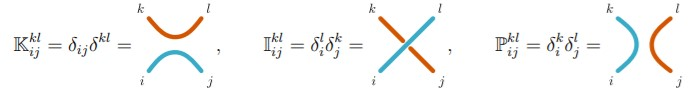
\includegraphics[width=\linewidth]{1.jpg}
  \caption{Invariant tensors can be thought of as different channels of scattering. From \cite{1}}
  \label{fig:1}
\end{figure}
Defining the following projection operators,
$$
\begin{array}{l}
\mathbb{P}_{\text {sing }}=\mathbb{P}_{0}=\frac{1}{3} \delta_{a b} \delta^{c d} \\\\
\mathbb{P}_{\text {anti }}=\mathbb{P}_{1}=\frac{1}{2}\left(\delta_{a}^{c} \delta_{b}^{d}-\delta_{a}^{d} \delta_{b}^{c}\right) \\\\
\mathbb{P}_{\text {sym }}=\mathbb{P}_{2}=\frac{1}{2}\left(\delta_{a}^{c} \delta_{b}^{d}+\delta_{a}^{d} \delta_{b}^{c}-\frac{2}{3} \delta_{a b} \delta^{c d}\right)
\end{array}
$$
which satisfy $\mathbb{P}_{I} \mathbb{P}_{J}=\delta_{I J}\mathbb{P}_{I}$ and we see that
$$
\delta_{a b} \delta^{c d}\mathbb{P}_{\text {sing }}=\delta_{a b} \delta^{c d}\mathbb{P}_{0}=\frac{1}{3}\delta_{a b} \delta^{c d} \delta_{a b} \delta^{c d}=3
$$
$$
\delta_{a b} \delta^{c d}\mathbb{P}_{\text {anti}}=\delta_{a b} \delta^{c d}\mathbb{P}_{1}=\frac{1}{2}\delta_{a b} \delta^{c d}\left(\delta_{a}^{c} \delta_{b}^{d}-\delta_{a}^{d} \delta_{b}^{c}\right)=0
$$
$$
\delta_{a b} \delta^{c d}\mathbb{P}_{\text {sym }}=\delta_{a b} \delta^{c d}\mathbb{P}_{2}=\frac{1}{2}\delta_{a b} \delta^{c d}\left(\delta_{a}^{c} \delta_{b}^{d}+\delta_{a}^{d} \delta_{b}^{c}-\frac{2}{3} \delta_{a b} \delta^{c d}\right)=0
$$
and these traces gives them the label singlet, anti-symmetric and symmetric traceless. And also,
$$
\begin{array}{l}
\delta_{a b} \delta^{c d}=3\mathbb{P}_{0} \\\\
\delta_{a}^{c} \delta_{b}^{d}=\mathbb{P}_{0}+\mathbb{P}_{1}+\mathbb{P}_{2}\\\\
\delta_{a}^{d} \delta_{b}^{c}=\mathbb{P}_{0}-\mathbb{P}_{1}+\mathbb{P}_{2}
\end{array}
$$
gives us
$$
\begin{aligned}
\mathcal{T}=&(3 A(s|t, u)+A(t|s, u)+A(u|s, t)) \mathbb{P}_{0} \\
&+(A(t|s, u)-A(u|s, t)) \mathbb{P}_{1}+(A(t|s, u)+A(u|s, t)) \mathbb{P}_{2} \\
=& \mathcal{T}^{(0)} \mathbb{P}_{0}+ \mathcal{T}^{(1)} \mathbb{P}_{1}+ \mathcal{T}^{(2)} \mathbb{P}_{2} \\
=& \frac{16 \pi i \sqrt{s}}{\sqrt{s-4}} \sum_{I=0,1,2} \mathbb{P}_{I} \sum_{\ell}(2 \ell+1)\left(1-S_{\ell}^{(I)}(s)\right) P_{\ell}\left(\frac{u-t}{u+t}\right)
\end{aligned}
$$
The second equality is a definition which can be rewritten as 
$$
S_{\ell}^{(I)}(s)=1+\left.i \frac{\sqrt{s-4}}{\sqrt{s}} \int_{-1}^{1} d x \frac{P_{\ell}(x)}{32 \pi} \mathcal{T}^{(I)}(s, t)\right|_{t \rightarrow \frac{1}{2}(s-4)(x-1)}=1+2 i \frac{\sqrt{s-4}}{\sqrt{s}} \mathcal{T}_{l}^{(I)}
$$
which looks similar to the following for $d=3$ (here $d$ is number of spacelike dimensions)
$$
S_{\ell}(s)=1+\left.i \frac{(s-4)^{\frac{d}{2}}}{\sqrt{s}} \int_{-1}^{1} d x\left(1-x^{2}\right)^{\frac{d-3}{2}} P_{\ell}^{(d)}(x)\mathcal{T}(s, t)\right|_{t \rightarrow \frac{1}{2}(s-4)(x-1)}
$$















\subsection{Partial Wave Unitarity Bounds}
To derive partial wave unitarity bounds \cite{4}, we use optical theorem to get
$$
\begin{aligned}
\operatorname{Im} \mathcal{T}(\pi \pi \rightarrow \pi \pi) &=2 E_{C M}\left|\vec{p}_{i}\right| \sum_{X} \sigma_{t o t}(\pi \pi \rightarrow X) \\
& \geq 2 E_{C M}\left|\vec{p}_{i}\right| \sigma_{t o t}(\pi \pi \rightarrow \pi \pi)
\end{aligned}
$$
where $\sigma_{\mathrm{tot}}(\pi \pi \rightarrow \pi \pi)=\frac{1}{64 \pi E_{\mathrm{CM}}^{2}} \int d( \cos \theta)|\mathcal{\mathcal{T}}(\theta)|^{2}$ where extra factor of $\frac{1}{2}$ w.r.t. equation in \cite{4} comes from the fact that particles are identical and hence there is an overcounting by factor of $2$ in summing over states.\\\\ And we can also write 
$$
 \mathcal{T}_{l}^{(I)}= \frac{1}{2} \int_{-1}^{1} d x \frac{P_{\ell}(x)}{32 \pi} \mathcal{T}^{(I)}(s, t)=\frac{S_{\ell}^{(I)}(s)-1}{2i} \frac{\sqrt{s}}{\sqrt{s-4}}
$$
and 
$$\mathcal{T}^{(I)}=32 \pi \sum_{\ell} \mathcal{T}^{(I)}_{\ell}(2 \ell+1) P_{\ell}(\cos (\theta))$$
Writing optical theorem in terms of the isospin projection operators, 
$$\operatorname{Im} \mathcal{T}(\pi \pi \rightarrow \pi \pi)=\sum_{I} \operatorname{Im} \mathcal{T}^{(I)}(\pi \pi \rightarrow \pi \pi) \mathbb{P}_{I}$$
and
$$|\mathcal{T}(\pi \pi \rightarrow \pi \pi)|^{2}=\sum_{I,J}  \mathcal{T}^{(I)}(\pi \pi \rightarrow \pi \pi) \mathbb{P}_{I} \mathcal{T}^{(J)}(\pi \pi \rightarrow \pi \pi) \mathbb{P}_{J} $$
Using $\mathbb{P}_{I} \mathbb{P}_{J}=\delta_{I J} \mathbb{P}_{I}$,
$$|\mathcal{T}(\pi \pi \rightarrow \pi \pi)|^{2}=\sum_{I,J} | \mathcal{T}^{(I)}(\pi \pi \rightarrow \pi \pi)|^{2} \mathbb{P}_{I}  $$
The equation
$$ \operatorname{Im} \mathcal{T}(\pi \pi \rightarrow \pi \pi)  \geq 2 E_{C M}\left|\vec{p}_{i}\right| \frac{1}{64 \pi E_{\mathrm{CM}}^{2}} \int d(\cos \theta)|\mathcal{T}(\pi \pi \rightarrow \pi \pi)|^{2}$$
implies by equating coefficients of projection operators
$$ \operatorname{Im} \mathcal{T}^{(I)}(\pi \pi \rightarrow \pi \pi)  \geq 2 E_{C M}\left|\vec{p}_{i}\right| \frac{1}{64 \pi E_{\mathrm{CM}}^{2}} \int d(\cos \theta)|\mathcal{T}^{(I)}(\pi \pi \rightarrow \pi \pi)|^{2}=2 E_{C M}\left|\vec{p}_{i}\right|\sigma_{\text {tot }}^{(I)}(\pi \pi \rightarrow \pi \pi) $$
where second inequality is a definition.
$$\begin{aligned} \sigma^{(I)}_{\text {tot }}(\pi \pi \rightarrow \pi \pi) &=\frac{(32 \pi)^{2}}{64 \pi E_{C M}^{2}} \sum_{l,l'} \int d (\cos \theta) \mathcal{T}^{(I)}_{l} \mathcal{T}_{l'}^{(I)*}(2 l+1)(2 l'+1) P_{l}(\cos \theta) P_{l'}(\cos \theta) \\
 &=\frac{16 \pi}{E_{C M}^{2}}  \sum_{l,l'}(2 l+1)(2 l'+1) \mathcal{T}^{(I)}_{l} \mathcal{T}_{l'}^{(I)*} \frac{2}{2 l+1} \delta_{l,l'} \\ 
&=\frac{32 \pi}{E_{C M}^{2}} \sum_{l}(2 l+1)\left|\mathcal{T}^{(I)}_{l}\right|^{2} \end{aligned}$$
$$\operatorname{Im}\mathcal{T}^{(I)}=32 \pi \sum_{\ell} \operatorname{Im}\mathcal{T}^{(I)}_{\ell}(2 \ell+1) P_{\ell}(\cos \theta)$$
Using optical theorem for $\theta=0$,
$$\begin{aligned} \sum_{l}(2 l+1) \operatorname{Im}\left(\mathcal{T}^{(I)}_{l}\right) & \geq \frac{2\left|\vec{p}_{i}\right|}{E_{C M}} \sum_{l}(2 l+1)\left|\mathcal{T}^{(I)}_{l}\right|^{2} \\ & \geq \frac{\sqrt{s-4}}{\sqrt{s}} \sum_{l}(2 l+1)\left|\mathcal{T}^{(I)}_{l}\right|^{2} \end{aligned}$$
Term by term comparision gives
$$\operatorname{Im}\left(\mathcal{T}^{(I)}_{l}\right) \geq \frac{\sqrt{s-4}}{\sqrt{s}} \left|\mathcal{T}^{(I)}_{l}\right|^{2} $$
Now we use $\mathcal{T}_{l}^{(I)}=\frac{S_{l}^{(I)}(s)-1}{2 i} \frac{\sqrt{s}}{\sqrt{s-4}}\Rightarrow \operatorname{Im}\left(\mathcal{T}^{(I)}_{j}\right)=-\frac{\operatorname{Re}\left(S^{(I)}_{l}(s)-1\right)}{2} \frac{\sqrt{s}}{\sqrt{s-4}}$ to get
$$-\frac{\operatorname{Re}\left(S^{(I)}_{l}(s)-1\right)}{2} \frac{\sqrt{s}}{\sqrt{s-4}} \geq \frac{\sqrt{s-4}}{\sqrt{s}} \frac{\left(S^{(I)}_{l}(s)-1\right)(S^{(I)*}_{l}(s)-1)}{4} \frac{s}{s-4}$$
$$\Rightarrow-2 \operatorname{Re}\left(S^{(I)}_{l}(s)\right)+2 \geq\left|S^{(I)}_{l}(s)\right|^{2}+1-\left(S^{(I)}_{l}(s)+S^{(I)*}_{l}(s)\right)$$
Hence we have the partial wave unitarity bounds for all $I$ and $l$ and all $s>4$
$$\left|S^{(I)}_{l}(s)\right|^{2} \leq 1$$
\subsection{Ansatz for $A(s|t,u)$}
Transformaing from $s,t,u \mapsto \rho_{s},\rho_{t},\rho_{u}$ as shown in Appendix A, we can write down an ansatz for $A(s|t,u)$ which is crossing symmetric i.e. $A(s|t,u)=A(s|u,t)$ as
$$
A(s | t, u)=\sum_{n \leq m}^{\infty} a_{n m}\left(\rho_{t}^{n} \rho_{u}^{m}+\rho_{t}^{m} \rho_{u}^{n}\right)+\sum_{n, m}^{\infty} b_{n m}\left(\rho_{t}^{n}+\rho_{u}^{n}\right) \rho_{s}^{m}
$$
with $\rho_{z} = \frac{\sqrt{\frac{8}{3}}-\sqrt{4-z}}{\sqrt{\frac{8}{3}}+\sqrt{4-z}}$\\\\















\subsection{SDPB}
We use SDPB that solves the following problem \cite{3}:
$$
\begin{array}{l}
\text { maximize } a \cdot z \text { over } z \in \mathbb{R}^{N+1},\\
\text { such that } \sum_{n=0}^{N} z_{n} W_{j}^{n}(x) \succeq 0 \quad \text { for all } x \geq 0 \text { and } 1 \leq j \leq J\\
\text{ with normalization }n.z=1
\end{array}
$$
To impose unitarity in SDPB \cite{5}, we write scattering amplitude (with poles subtracted off if any) as
$$
M(s, t, 4-s-t)=\vec{\eta} \cdot \vec{M}(s, t)
$$
where $\vec{\eta}$ is a vector containing all parameters in the ansatz (like all $a_{n m}, b_{n m}$ in case of pion bootstrap) after the truncation at $a+b \leq N_{max}$ and $l \leq L_{max}$ and this unitarity constraint is imposed at various points (say 200-300 points on the unit circle in $\rho$-plane which corresponds to different real values of $s(>4)$). After integrating $M$ with Legendre polynomials, one can write it symbolically as (suppresing isospin indices in case of pion bootstrap as each has to be contrained individually)
$$
S_{l}(s)=1+\iota \vec{\eta} \cdot \vec{\mathcal{T}}_{l}(s)
$$
Defining $\vec{R}=\operatorname{Re}\left[\vec{\mathcal{T}_{\ell}(s)}\right]$ and $\vec{I}=\operatorname{Im}\left[\vec{\mathcal{T}_{\ell}(s)}\right]$, we can write $|S_{l}(s)|^{2}\leq 1$ as
$$(1-\vec{\eta} \cdot \vec{I})^{2}+(\vec{\eta} \cdot \vec{R})^{2} \leq 1 \quad \Rightarrow \quad U \equiv 2 \vec{\eta} \cdot \vec{I}-(\vec{\eta} \cdot \vec{I})^{2}-(\vec{\eta} \cdot \vec{R})^{2} \geq 0$$
And this is equivalent to semi-definiteness of 
$$
M:=\left(\begin{array}{cc}
1+\vec{\eta} \cdot \vec{R} & 1-\vec{\eta} \cdot \vec{I} \\
1-\vec{\eta} \cdot \vec{I} & 1-\vec{\eta} \cdot \vec{R}
\end{array}\right)
$$
whose entries are an input into SDPB program. \\\\
The imposition of unitarity gives a general S-matrix. To bring in inputs about pions, we use experimental values like $\rho$ resonance. To impose $\rho$ resonance condition $S_{1}^{(1)}\left(m_{\rho}^{2}\right)=0$ where $m_{\rho}^{2} \in \mathbb{C}$, we have 
$$\mathcal{T}_{1}^{(1)}\left(m_{\rho}^{2}\right)=-i$$
with factors of $2 \frac{\sqrt{s-4}}{\sqrt{s}}$ subsumed into $\mathcal{T}$. This is imposed by setting imaginary part $=-1$ and real part $=0$ for Isospin =1 and $l=1$ which is equivalent to semi-definiteness of
$$
M:=\left(\begin{array}{cc}
\vec{\eta} \cdot \vec{R_{1}} & 0 \\
0& -\vec{\eta} \cdot \vec{R_{1}}
\end{array}\right)
$$
and
$$
M:=\left(\begin{array}{cc}
\vec{\eta} \cdot \vec{I_{1}}+1 & 0 \\
0& -\vec{\eta} \cdot \vec{I_{1}}-1
\end{array}\right)
$$
and we have at sub-threshold regions, characteristic weak coupling conditions (Amplitude $\rightarrow$ 0) called Adler Zeroes. For imposition of Adler Zeroes
$$
S_{0}^{(0)}\left(s_{0}\right)=S_{0}^{(2)}\left(s_{2}\right)=1
$$
we need 
$$
\mathcal{T}_{0}^{(0)}\left(s_{0}\right)=\mathcal{T}_{0}^{(2)}\left(s_{2}\right)=0
$$
which can be imposed by setting Real and Imaginary parts for $I=0,2;l=0$ using equivalence to semi-definiteness of
$$
M:=\left(\begin{array}{cc}
\vec{\eta} \cdot \vec{R_{0}}(/\vec{I_{0}}) & 0 \\
0& -\vec{\eta} \cdot \vec{R_{0}}(/\vec{I_{0}}) 
\end{array}\right)
$$
Lastly to impose $|a-b|\leq \epsilon$
$$
M:=\left(\begin{array}{cc}
a-b-\epsilon & 0 \\
0&b-a-\epsilon 
\end{array}\right)
$$
\textbf{NOTE}:- If a constraint is identically zero (say, if $\operatorname{Re} \mathcal{T}_{1}^{(1)} = 0$), then imposing that in SDPB gives an error. 


















\subsection{Fun Facts}
Leading order ChiPT gives us \cite{2} 
$$
\mathcal{T}_{0}^{(0)}=\frac{2 s-1}{32 \pi f_{\pi}^{2}}, \quad \mathcal{T}_{0}^{(2)}=\frac{2-s}{16 \pi f_{\pi}^{2}}, \quad \mathcal{T}_{1}^{(1)}=\frac{s-4}{96 \pi f_{\pi}^{2}}
$$
where $ f_{\pi}$ is pion decay constant. Tree level Adler zeros are hence at $s_{0}=1 / 2 \text { and } s_{2}=2$.\\\\
At low energies, the partial wave can be expanded in $k=\sqrt{\frac{s-4}{4}}$ which the momentum in center of mass frame.
$$
\operatorname{Re}\left[\mathcal{T}_{\ell}^{(I)}\right]=k^{2 \ell}\left[a_{\ell}^{(I)}+b_{\ell}^{(I)} k^{2}+\mathcal{O}\left(k^{4}\right)\right]
$$
$a_{\ell}^{(I)}$'s are called scattering lengths and $b_{\ell}^{(I)}$'s effective ranges. These have been measured experimentally.
\begin{center}
\begin{tabular}{ |c|c|c| } 
 \hline
 I&$\mathcal{O}(k^{0})$&$\mathcal{O}(k^{2})$\\
 0 & $a_{0}^{(0)}=0.2196\pm 0.0034$ & $b_{0}^{(0)}=0.276\pm 0.006$ \\ 
 1 &  & $a_{1}^{(1)}=0.038\pm 0.002$ \\ 
 2 & $a_{0}^{(2)}=-0.0444\pm 0.0012$ & $b_{0}^{(2)}=-0.0803\pm 0.0012$ \\ 
 \hline
\end{tabular}
\end{center}

















\subsection{Lake}
Adler zeroes occur in the unphysical region $s<4$ and hence they can't be measured in an experiment. And we would like to find S-matrices that have two Adler Zeroes, a $\rho$ resonance and satisfy unitarity for all isospin channels. To do this we first fix $s_{0}$. Then impose the following\\\\
1. Unitarity\\
2. One Adler Zero $\mathcal{T}_{0}^{(0)}(s_{0})=0$\\
3. $\rho$ resonance at $S_{1}^{(1)}(m_{\rho}^{2})=0$ at $m_{\rho}^{2}=5.5+0.5i$\\\\
We want the maximum and minimum value $\mathcal{T}_{0}^{(2)}(s)$. So we choose $a$ such that $a\cdot z=\mathcal{T}_{0}^{(2)}(s)$ for maximizing and replace $a\rightarrow -a$ to get maximum of $-\mathcal{T}_{0}^{(2)}(s)$ which is minimum of $\mathcal{T}_{0}^{(2)}(s)$. At the values of $s$ where both maximum and minimum has the same sign, it will not be possible to impose the 2nd Adler Zero. We do this for a number of points $0<s<4$ and get an excluded region where two Adler zeroes can't be imposed.
\begin{figure}[H]
    \centering
    \subfloat[\centering Plots of Maximum and Minimum values for a fixed $s_{0}$(here$=0.5$) and excluded region marked red and dubbed a Lake.]{{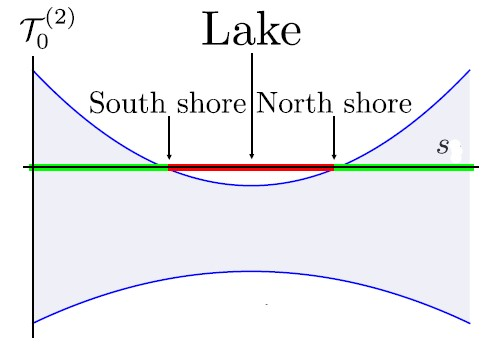
\includegraphics[width=6cm]{3.jpg} }}
    \qquad
    \subfloat[\centering White region is where 2 Adler zeroes can't be imposed. Black dot denotes the tree level ChiPT Adler zeroes.]{{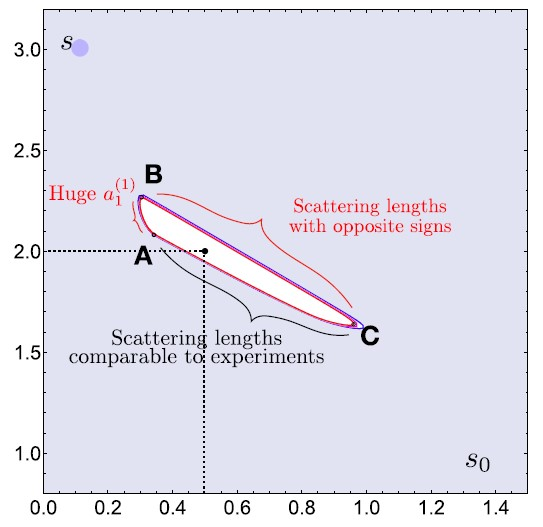
\includegraphics[width=6cm]{4.jpg} }}
    \caption{From \cite{2}}
    \label{fig:example}
\end{figure}
Interestingly, the tree level ChiPT point lies well within exculded region. This is explained by noting that physis of resonance which is a strong coupling phenomena can't be realized at tree level which is a weak coupling limit.
\begin{figure}[H]
  \centering
  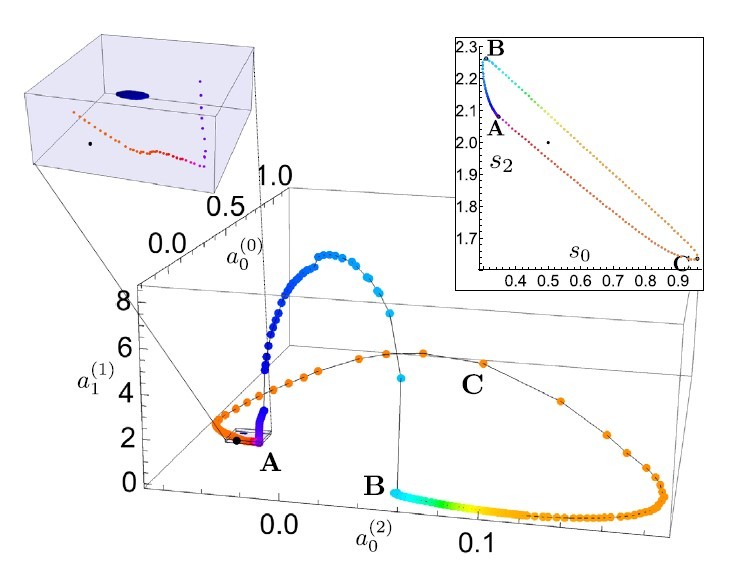
\includegraphics[width=8cm]{5.jpg}
  \caption{Scattering lengths along Lake boundary. From \cite{2}}
  \label{fig:1}
\end{figure}
We see that the lower boundary of the Lake is where scattering lengths are close to the tabulated values. So we now impose those experimental values in the next section.















\subsection{Peninsula}
Here we impose all constraints used in the Lake plus the experimental scattering length values $\left|a_{0}^{(0)}-0.2196\right|<0.034$, $\left|a_{1}^{(1)}-0.038\right|<0.002$ and $\left|a_{0}^{(2)}-(-0.0444)\right|<0.0012$, a total of 6 extra constraints and the allowed region is as expected near the lower boundary of the Lake region (but outside it as all constraints used in Lake are used here).
\begin{figure}[H]
    \centering
    \subfloat[\centering Plots of Maximum and Minimum values for a fixed $s_{0}$(here$=0.5$).]{{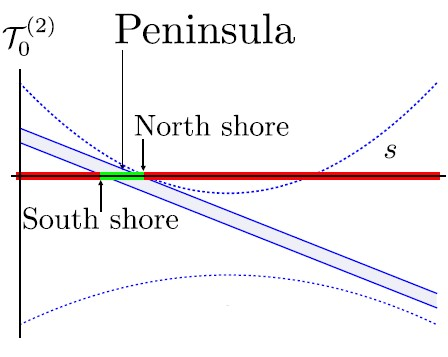
\includegraphics[width=6cm]{7.jpg} }}
    \qquad
    \subfloat[\centering Peninsula]{{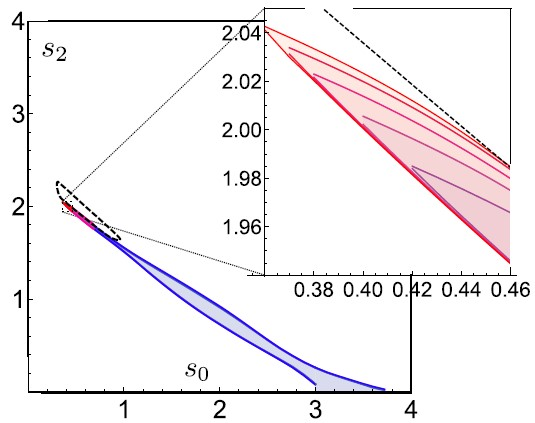
\includegraphics[width=6cm]{6.jpg} }}
    \caption{From \cite{2}}
    \label{fig:example}
\end{figure}










\subsection{River}






\subsubsection{Pion Scattering Amplitudes}
$$
\pi^{0}=|0\rangle \quad \pi^{\pm}=\frac{1}{\sqrt{2}}[|1\rangle \pm i|2\rangle]
$$
Using Projection operators' expressions,\\
1. $a=b=c=d$\\
$\mathbb{P}^{0}=\frac{1}{3} \qquad \mathbb{P}^{1}=0 \qquad \mathbb{P}^{2}=\frac{2}{3}$\\
2. $a=c\neq b=d$\\
$\mathbb{P}^{0}=0 \qquad \mathbb{P}^{1}=\frac{1}{2} \qquad \mathbb{P}^{2}=\frac{1}{2}$\\
3. $a=d \neq b=c$\\
$\mathbb{P}^{0}=0 \qquad \mathbb{P}^{1}=-\frac{1}{2} \qquad \mathbb{P}^{2}=\frac{1}{2}$\\
4. $a=b\neq c=d$\\
$\mathbb{P}^{0}=\frac{1}{3} \qquad \mathbb{P}^{1}=0 \qquad \mathbb{P}^{2}=-\frac{1}{3}$\\
5. The ones without two pairs of equal numbers are zero.\\\\
$$\mathcal{M}(\pi^{0} \pi^{0} \rightarrow \pi^{0}\pi^{0})=\langle00|\mathcal{T}|00\rangle$$
Since $a=b=c=d=0$, $\mathbb{P}^{0}=\frac{1}{3} \qquad \mathbb{P}^{1}=0 \qquad \mathbb{P}^{2}=\frac{2}{3}$ and so,
$$\mathcal{M}(\pi^{0} \pi^{0} \rightarrow \pi^{0}\pi^{0})=\frac{\mathcal{T}^{(0)}}{3}+\frac{2\mathcal{T}^{(2)}}{3}$$
$$\Rightarrow \mathcal{M}(\pi^{0} \pi^{0} \rightarrow \pi^{0}\pi^{0})=\frac{3 A(s|t, u)+A(t|s, u)+A(u|s, t)}{3}+\frac{2(A(t|s, u)+A(u|s, t))}{3}$$
$$\Rightarrow \mathcal{M}(\pi^{0} \pi^{0} \rightarrow \pi^{0}\pi^{0})=A(s|t, u)+A(t|s, u)+A(u|s, t)$$
\\\\
$$\mathcal{M}(\pi^{+} \pi^{0} \rightarrow \pi^{+}\pi^{0})=\frac{1}{2} \left[\langle10|\mathcal{T}|10\rangle+\langle20|\mathcal{T}|20\rangle+(\text{vanishing terms due to point 5})\right]$$
Since $a=c\neq b=d$, $\mathbb{P}^{0}=0 \qquad \mathbb{P}^{1}=\frac{1}{2} \qquad \mathbb{P}^{2}=\frac{1}{2}$ and so,
$$\mathcal{M}(\pi^{+} \pi^{0} \rightarrow \pi^{+}\pi^{0})=\frac{\mathcal{T}^{(1)}}{2}+\frac{\mathcal{T}^{(2)}}{2}$$
$$\Rightarrow \mathcal{M}(\pi^{+} \pi^{0} \rightarrow \pi^{+}\pi^{0})=\frac{A(t|s, u)-A(u|s, t)}{2}+\frac{A(t|s, u)+A(u|s, t)}{2}$$
$$\Rightarrow \mathcal{M}(\pi^{+} \pi^{0} \rightarrow \pi^{+}\pi^{0})=A(t|s, u)$$
\\\\
$$\begin{aligned} \mathcal{M}(\pi^{+} \pi^{+} \rightarrow \pi^{+}\pi^{+})=&\frac{1}{4} \left[\langle11|\mathcal{T}|11\rangle-\langle22|\mathcal{T}|12\rangle+\langle12|\mathcal{T}|11\rangle+\langle21|\mathcal{T}|12\rangle\right. \\
&\left.+\langle12|\mathcal{T}|21\rangle+\langle21|\mathcal{T}|21\rangle-\langle22|\mathcal{T}|11\rangle+\langle22|\mathcal{T}|22\rangle \right.\\
&\left.+(\text{vanishing terms due to point 5})\right] \end{aligned}$$
Using all the cases and adding up,  
$$\mathcal{M}(\pi^{+} \pi^{+} \rightarrow \pi^{+}\pi^{+})=\mathcal{T}^{(2)}$$
$$\Rightarrow \mathcal{M}(\pi^{+} \pi^{+} \rightarrow \pi^{+}\pi^{+})=A(t|s, u)+A(u|s, t)$$
It can also be diagrammatically obtained as shown in fig.
\begin{figure}[H]
  \centering
  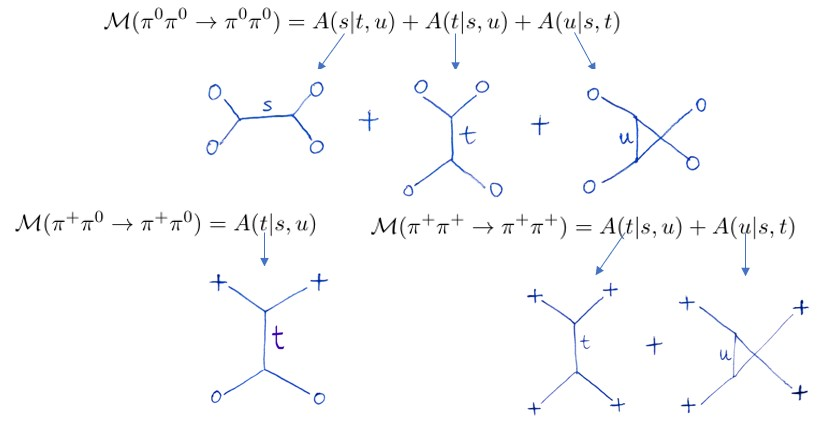
\includegraphics[width=12cm]{8.jpg}
  \caption{}
  \label{fig:1}
\end{figure}










\subsubsection{Crossing Matrix}
We follow the discussion in \cite{6}.\\
For the process $a\left(p_{a}\right)+b\left(p_{p}\right) \rightarrow$ $c\left(p_{c}\right)+d\left(p_{d}\right)$,
$$
\mathcal{T}_{a b}^{c d}=A(s|t, u) \delta_{a b} \delta^{c d}+A(t|s, u) \delta_{a}^{c} \delta_{b}^{d}+A(u|s, t) \delta_{a}^{d} \delta_{b}^{c}
$$
We define $A(s|t, u)=A(s|u,t)\equiv A(s,t)=A(s,u)=A(s,4m^{2}-s-t)$. With this we can write
$$
\begin{aligned}
&\mathcal{T}^{0}(s, t)=3 A(s, t)+A(t, s)+A(u, s) \\
&\mathcal{T}^{1}(s, t)=A(t, s)-A(u, s) \\
&\mathcal{T}^{2}(s, t)=A(t, s)+A(u, s)
\end{aligned}
$$
We can easily see that under exchange in final states, $\mathcal{T}^{0}(s, t)=\mathcal{T}^{0}(s, u), \quad \mathcal{T}^{1}(s, t)=-\mathcal{T}^{1}(s, u), \quad \mathcal{T}^{2}(s, t)=\mathcal{T}^{2}(s, u)$.\\\\
We will need the relation between $\mathcal{T}(s, t)$ and $\mathcal{T}(u,t)$ and also $\mathcal{T}(s, t)$ and $\mathcal{T}(t,s)$.
$$
\begin{aligned}
&\mathcal{T}^{0}(u, t)=3 A(u, t)+A(t, u)+A(s,u) \\
&\mathcal{T}^{1}(u, t)=A(t, u)-A(s,u) \\
&\mathcal{T}^{2}(u, t)=A(t, u)+A(s,u)
\end{aligned}
$$
$$
\begin{aligned}
&\mathcal{T}^{0}(u, t)-\mathcal{T}^{2}(u, t)=3 A(u, t)=3 A(u, s) \\
&\mathcal{T}^{1}(u, t)+\mathcal{T}^{2}(u, t)=2A(t, u)=2A(t, s)\\
&\mathcal{T}^{2}(u, t)-\mathcal{T}^{1}(u, t)=2A(s,u)=2A(s,t)
\end{aligned}
$$
Knowing $A(u, s), A(t, s), A(s, t)$ we can write $\mathcal{T}(s, t)=C \mathcal{T}(u, t)$.
$$
\begin{aligned}
&T^{I}(s, t) =C_{u}^{I I^{\prime}} T^{I^{\prime}}(u, t) \\
&C_{u}^{I I^{\prime}} C_{u}^{I^{\prime} J} =\delta_{I J} \\
&C_{u} =\frac{1}{6}\left(\begin{array}{rrr}
2 & -6 & 10 \\
-2 & 3 & 5 \\
2 & 3 & 1
\end{array}\right)
\end{aligned}
$$
Similarly for crossed t-channel,
$$
\begin{aligned}
&T^{I}(s, t) =C_{t}^{I I^{\prime}} T^{I^{\prime}}(t, s) \\
&C_{t}^{I I^{\prime}} C_{t}^{I^{\prime} J} =\delta_{I J} \\
&C_{t} =\frac{1}{6}\left(\begin{array}{rrr}
2 & 6 & 10 \\
2 & 3 & -5 \\
2 & -3 & 1
\end{array}\right)
\end{aligned}
$$












\subsubsection{Analyticity in Mandelstram Plane}
In the complex $s$-plane, the scattering amplitudes are analytic everywhere except for a few isolated points and branch cuts due to unitarity. If $s_{0}$ is smallest branch point on real axis, we will have branch cut for $s \geq s_{0}$. Other branch cuts will be obtained using crossing symmetry. Above the mass threshold for particle exchanges, the physical amplitude is defined as $T^{\text {phys }}(s, t)=$ $T(s+i \epsilon, t)$ (Feynman prescription). Schwarz reflection principle gives
$$
T^{*}(s+i \epsilon)=T(s-i \epsilon) \Rightarrow  T(s+i \epsilon)-T(s-i \epsilon)=2 i \operatorname{Im} T(s+i \epsilon) \neq 0
$$
Last step is since optical theorem relates $\operatorname{Im} T(s+i \epsilon)$ to deacy rates which are non-zero above the threshold. This non-analyticity for $s \geq 4m^{2}$ will translate into crossed channels to give \\\\
1. \textbf{Non-analytic for $s,t,u \geq 4m^{2}$ OR Analytic for  $s,t \leq 4m^{2}, s+t \geq 0$}












\subsubsection{Fixed $t$ Dispersion Relation}
Cauchy's Theorem in complex $s$-plane keeping $t$ fixed can be used to write
$$T^{I}(s, t)=\frac{1}{2 \pi i} \oint_{\gamma} \mathrm{d} x \frac{T^{I}(x, t)}{x-s}$$
The neighbourhood (in $s$) of $(s,t)$ must be analytic and hence $t<4m^{2}$. Branch cuts are at $s>4m^{2}$ and the crossing counterpart at $s<-t$.
\begin{figure}[H]
  \centering
  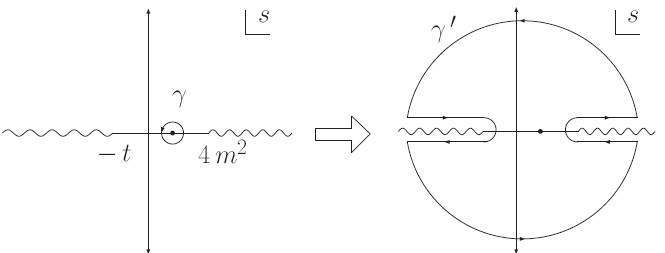
\includegraphics[width=12cm]{9.jpg}
  \caption{Scattering lengths along Lake boundary. From \cite{2}}
  \label{fig:1}
\end{figure}
The contour can be deformed to $\gamma'$. And if the semi-circle contours at infinity don't contribut this contour's contribution will be in terms of the discontinuity of amplitude along real axis which in turn is proportional to imaginary part of ampitude. If the amplitude does not vanish sufficiently fast one can use higher derivatives until eventually the semicircular contours don't contribute.
$$
\frac{\mathrm{d}^{n}}{\mathrm{~d} s^{n}} T^{I}(s, t)=\frac{n !}{2 \pi i} \oint_{\gamma} \mathrm{d} x \frac{T^{I}(x, t)}{(x-s)^{n+1}}
$$
Now we can write 
$$
\frac{\mathrm{d}^{n}}{\mathrm{~d} s^{n}} T^{I}(s, t)=\frac{n !}{2\pi i} \left[  \int_{4 m^{2}}^{\infty} \mathrm{d} x\frac{ 2i \operatorname{Im} T^{I}(x+i \epsilon, t)}{(x-s)^{n+1}} - \int_{-t}^{-\infty} \mathrm{d} x\frac{ 2i \operatorname{Im} T^{I}(x+i \epsilon, t)}{(x-s)^{n+1}}  \right]
$$
Changing variables in second integral to $y=4m^{2}-t-x$, we get $dx=-dy$ and $x-s=4m^{2}-t-s-y=u-y=-(y-u)$
$$
\frac{\mathrm{d}^{n}}{\mathrm{~d} s^{n}} T^{I}(s, t)=\frac{n !}{\pi } \left[  \int_{4 m^{2}}^{\infty} \mathrm{d} x\frac{  \operatorname{Im} T^{I}(x+i \epsilon, t)}{(x-s)^{n+1}} -(-1)^{n} \int_{4 m^{2}}^{\infty}  \mathrm{d} y\frac{ \operatorname{Im} T^{I}(4m^{2}-t-y+i \epsilon, t)}{(y-u)^{n+1}}  \right]
$$
$$
T^{I}(s, t)=C_{u}^{I I^{\prime}} T^{I^{\prime}}(u, t)=C_{u}^{I I^{\prime}} T^{I^{\prime}}(4m^{2}-t-s, t)
$$
Since $C_{u}$ is it's own inverse,
$$
\Rightarrow T^{I}(4m^{2}-t-y+i\epsilon, t)=T^{I}(4m^{2}-t-(y-i\epsilon), t)=C_{u}^{I I^{\prime}} T^{I^{\prime}}(y-i\epsilon, t)
$$
$$
\Rightarrow \operatorname{Im} T^{I}(4m^{2}-t-y+i\epsilon, t)=C_{u}^{I I^{\prime}} \operatorname{Im}T^{I^{\prime}}(y-i\epsilon, t)=-C_{u}^{I I^{\prime}} \operatorname{Im} T^{I^{\prime}}(y+i\epsilon, t)
$$
Last step was using Schwarz reflection principle. Renaming $y$ as $x$,
$$
\frac{\mathrm{d}^{n}}{\mathrm{~d} s^{n}} T^{I}(s, t)=\frac{n !}{\pi} \int_{4 m^{2}}^{\infty} \mathrm{d} x\left[\frac{\delta^{I I^{\prime}}}{(x-s)^{n+1}}\right. \left.+(-1)^{n} \frac{C_{u}^{I I^{\prime}}}{(x-u)^{n+1}}\right] \operatorname{Im} T^{I^{\prime}}(x+i \epsilon, t)
$$
The equation with the least value of $n$ for which the semicircular contours vanish is the strongest constraint. Both denominators are positive at all integration points since we restrict to $s<4 m^{2}$ and $s+t>0$.
$$T^{I}(s, t) =\sum_{\ell=0}^{\infty}(2 \ell+1) f_{\ell}^{I}(s) P_{\ell}(\cos \theta) =\sum_{\ell=0}^{\infty}(2 \ell+1) f_{\ell}^{I}(s) P_{\ell}\left(1+\frac{2 t}{s-4 m^{2}}\right)$$
Optical theorem gives in terms of partial wave cross-sections $\sigma_{\ell}^{I}(s)$
$$
\operatorname{Im} f_{\ell}^{I}(s)=s \sqrt{1-\frac{4 m^{2}}{s}} \sigma_{\ell}^{I}(s) \geq 0
$$
$$
\operatorname{Im} T^{I}(s, t)=\sum_{\ell=0}^{\infty}(2 \ell+1) s \sqrt{1-\frac{4 m^{2}}{s}} \sigma_{\ell}^{I}(s) P_{\ell}\left(1+\frac{2 t}{s-4 m^{2}}\right)
$$
When $t>0$, $\frac{2 t}{s-4 m^{2}}>0$ and since analytically continued Legendre polynomial satisfies $P_{\ell}(z)>1$ if $z>1$, we make another restriction (apart from $s,t<4m^{2}$ and $s+t>0$),\\\\
2. \textbf{$\operatorname{Im} T^{I}(s, t)>0$ for $t>0$}\\\\
$s,t<4m^{2}, s+t>0, t>0$ define a region $\mathcal{A}$ in the Mandelstram Plane as shown in figure enclosed in black border.
\begin{figure}[H]
  \centering
  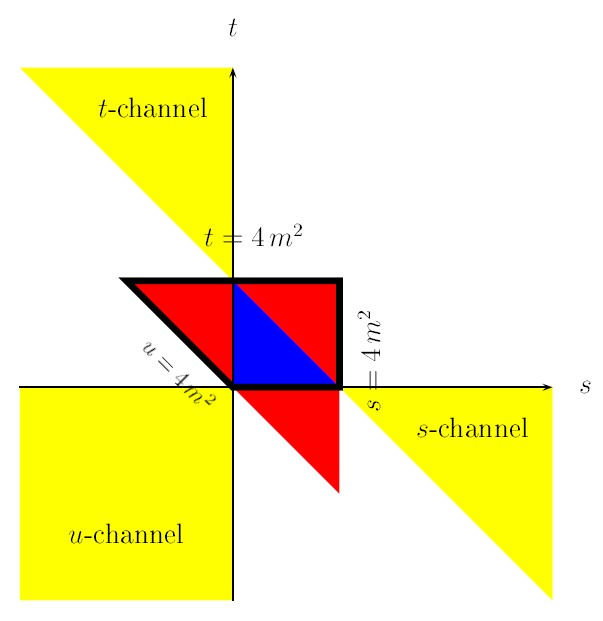
\includegraphics[width=9cm]{10.jpg}
  \caption{Region $\mathcal{A}$: Analyticity $+ \operatorname{Im} T^{I}(s, t)>0$. From \cite{6}}
  \label{fig:1}
\end{figure}
Furthermore Friossart bounds imply $n=2$ suffices for pion scattering \cite{6}. So factor of $(-1)^{n}=1>0$. \\\\
So the only thing left to check for $\frac{\mathrm{d}^{2}}{\mathrm{~d} s^{2}} T(s, t)>0$ is that the amplitude in question being $T=\sum a_{I} T^{I}$ should have $a_{I} \geq 0$ and also additionally $\sum a_{I} C_{u}^{I J} T_{J} \equiv \sum_{J} b_{J} T_{J}$ having $b_{J}=\sum_{I} a_{I} C_{u}^{I J} \geq 0.$\\\\
For $\mathcal{M}\left(\pi^{0} \pi^{0} \rightarrow \pi^{0} \pi^{0}\right)=\frac{\mathcal{T}^{(0)}}{3}+\frac{2 \mathcal{T}^{(2)}}{3}$,
$$
\begin{array}{l}
a=\left(\begin{array}{lll}
\frac{1}{3} & 0 & \frac{2}{3}
\end{array}\right) \\
b=a C_{u}=\frac{1}{6}\left(\begin{array}{lll}
\frac{1}{3} & 0 & \frac{2}{3}
\end{array}\right)\left(\begin{array}{ccc}
2 & -6 & 10 \\
-2 & 3 & 5 \\
2 & 3 & 1
\end{array}\right) \\
=\frac{1}{6}\left(\begin{array}{lll}
2 & 0 & 4
\end{array}\right) =\left(\begin{array}{lll}
\frac{1}{3} & 0 & \frac{2}{3}
\end{array}\right) 
\end{array}
$$
For $\mathcal{M}\left(\pi^{+} \pi^{0} \rightarrow \pi^{+} \pi^{0}\right)=\frac{\mathcal{T}^{(1)}}{2}+\frac{\mathcal{T}^{(2)}}{2}$,
$$
\begin{array}{l}
a=\left(\begin{array}{lll}
0 & \frac{1}{2} & \frac{1}{2}
\end{array}\right) \\
b=a C_{u}=\frac{1}{6}\left(\begin{array}{lll}
0 & \frac{1}{2} & \frac{1}{2}
\end{array}\right)\left(\begin{array}{ccc}
2 & -6 & 10 \\
-2 & 3 & 5 \\
2 & 3 & 1
\end{array}\right) \\
=\frac{1}{6}\left(\begin{array}{lll}
0 & 3 & 3
\end{array}\right) =\left(\begin{array}{lll}
0 & \frac{1}{2} & \frac{1}{2}
\end{array}\right) 
\end{array}
$$
For $\mathcal{M}\left(\pi^{+} \pi^{+} \rightarrow \pi^{+} \pi^{+}\right)=\mathcal{T}^{(2)}$,
$$
\begin{array}{l}
a=\left(\begin{array}{lll}
0 & 0 & 1
\end{array}\right) \\
b=a C_{u}=\frac{1}{6}\left(\begin{array}{lll}
0 & 0 & 1
\end{array}\right)\left(\begin{array}{ccc}
2 & -6 & 10 \\
-2 & 3 & 5 \\
2 & 3 & 1
\end{array}\right) \\
=\frac{1}{6}\left(\begin{array}{lll}
2 & 3 & 1
\end{array}\right) =\left(\begin{array}{lll}
\frac{1}{3} & \frac{1}{2} & \frac{1}{6}
\end{array}\right) 
\end{array}
$$
For all three amplitudes, all entries of both $a$ and $b$ are $\geq 0$. \\\\
This is expected since optical theorem ensures positivity of Imaginary part of partial wave since all three are processes with same initial and final states of the form $a+b \rightarrow a+b$ and crossing counterpart $a+\bar b \rightarrow a+\bar b$. So we have what we call \textbf{Positivity Conditions} or \textbf{Manohar Inequalities},
$$
\begin{aligned}
\frac{\mathrm{d}^{2}}{\mathrm{~d} s^{2}} T\left(\pi^{0} \pi^{0} \rightarrow \pi^{0} \pi^{0}\right)[(s, t) \in \mathcal{A}] \geq &0\\
\frac{\mathrm{d}^{2}}{\mathrm{~d} s^{2}} T\left(\pi^{+} \pi^{0} \rightarrow \pi^{+} \pi^{0}\right)[(s, t) \in \mathcal{A}] \geq &0 \\
\frac{\mathrm{d}^{2}}{\mathrm{~d} s^{2}} T\left(\pi^{+} \pi^{+} \rightarrow \pi^{+} \pi^{+}\right)[(s, t) \in \mathcal{A}] \geq &0
\end{aligned}
$$










\subsubsection{D-wave Inequalities from Positivity Relations}
We have the following expression for scattering lengths
$$
a_{\ell}^{I}=\lim _{s \rightarrow 4 m^{2}} \frac{f_{\ell}^{I}(s)}{\left(\frac{s}{4}-m^{2}\right)^{\ell}}
$$
$$
T^{I}(s, t)=\sum_{\ell=0}^{\infty}(2 \ell+1) f_{\ell}^{I}(s) P_{\ell}\left(1+\frac{2 t}{s-4 m^{2}}\right)
$$
$$
\left.\frac{\mathrm{d}^{\ell} T^{I}\left(s, t\right)}{\mathrm{d} t^{\ell}}\right|_{t=0}=\sum_{\ell=0}^{\infty}(2 \ell+1) f_{\ell}^{I}(s)\left(\frac{2}{s-4 m^{2}}\right)^{\ell}\left.\frac{\mathrm{d}^{\ell} P_{\ell}\left(x\right)}{\mathrm{d} x^{\ell}}\right|_{x=1}
$$
$\left.\frac{\mathrm{d}^{\ell} P_{\ell}\left(x\right)}{\mathrm{d} x^{\ell}}\right|_{x=1}$ is $l!$ times leading coefficient of Legendre polynomials which is equal to $\dfrac{(2\ell)!}{2^{\ell} \ell!}$.
$$
\lim _{s \rightarrow 4 m^{2}}\left.\frac{\mathrm{d}^{\ell} T^{I}\left(s, t\right)}{\mathrm{d} t^{\ell}}\right|_{t=0}=\sum_{\ell=0}^{\infty}(2 \ell+1) \left(f_{\ell}^{I}(s)\left(\frac{4}{s-4 m^{2}}\right)^{\ell}\right)\frac{(2\ell)!}{4^{\ell} \ell!}
$$
$$
\left.\frac{\mathrm{d}^{\ell} T^{I}\left(4 m^{2}, t\right)}{\mathrm{d} t^{\ell}}\right|_{t=0}=\sum_{\ell=0}^{\infty}a_{\ell}^{I}(2 \ell+1)! \frac{1}{4^{\ell} \ell!}
$$
(The following expression in \cite{6} has a typo)
$$
\begin{aligned}
a_{\ell}^{I} &=\left.\frac{4^{\ell} \ell !}{(2 \ell+1)!} \frac{\mathrm{d}^{\ell} T^{I}\left(4 m^{2}, t\right)}{\mathrm{d} t^{\ell}}\right|_{t=0} \\
&=\left.\frac{4^{\ell} \ell !}{(2 \ell+1)!} C_{t}^{I I^{\prime}} \frac{\mathrm{d}^{\ell} T^{I^{\prime}}\left(s, 4 m^{2}\right)}{\mathrm{d} s^{\ell}}\right|_{s=0}
\end{aligned}
$$
Inverse of $C_{t}$ is itself, so
$$
\left.\frac{\mathrm{d}^{\ell} T^{I}\left(s, 4 m^{2}\right)}{\mathrm{d} s^{\ell}}\right|_{s=0}=\frac{(2 \ell+1)!}{4^{\ell} \ell !} C_{t}^{I J} a_{\ell}^{J}
$$
For $l=2$ case, (this eqn. has a typo in \cite{6})
$$
\left.\frac{\mathrm{d}^{2} T^{I}\left(s, 4 m^{2}\right)}{\mathrm{d} s^{2}}\right|_{s=0}=\frac{120}{32} C_{t}^{I J} a_{2}^{J}
$$
$$
a_{\ell}^{I}=\left.\frac{4^{\ell} \ell !}{(2 \ell+1)!} \frac{\mathrm{d}^{\ell} T^{I}\left(4 m^{2}, t\right)}{\mathrm{d} t^{\ell}}\right|_{t=0}=\left.(-1)^{l}\frac{4^{\ell} \ell !}{(2 \ell+1)!} \frac{\mathrm{d}^{\ell} T^{I}\left(4 m^{2}, -t\right)}{\mathrm{d} t^{\ell}}\right|_{t=0}
$$
Using $T^{1}\left(4 m^{2}, t\right)=-T^{1}\left(4 m^{2},-t\right)$, for $l$ even we see
$$a_{l}^{1}=0$$
Since $(s,t)=(0,4m^{2})\in \mathcal{A}$, we have
$$
\begin{array}{l}
a_{2}^{I}=\left(\begin{array}{c}
a_{2}^{0} \\ 
0 \\
a_{2}^{2}
\end{array}\right)\\
C_{t}a_{2}=\frac{1}{6}\left(\begin{array}{ccc}
2 & 6 & 10 \\
2 & 3 & -5 \\
2 & -3 & 1
\end{array}\right)\left(\begin{array}{c}
a_{2}^{0} \\
0 \\
a_{2}^{2}
\end{array}\right) \\
\left.\frac{\mathrm{d}^{2} T\left(s, 4 m^{2}\right)}{\mathrm{d} s^{2}}\right|_{s=0}=\frac{120}{192}\left(\begin{array}{c}
2 a_{2}^{0} + 10 a_{2}^{2}\\
2 a_{2}^{0} - 5 a_{2}^{2}\\
2 a_{2}^{0} + a_{2}^{2}
\end{array}\right)
\end{array}
$$
For $\mathcal{M}\left(\pi^{0} \pi^{0} \rightarrow \pi^{0} \pi^{0}\right)=\frac{\mathcal{T}^{(0)}}{3}+\frac{2 \mathcal{T}^{(2)}}{3}$,
$$
\begin{aligned}
\frac{\mathrm{d}^{2}}{\mathrm{~d} s^{2}} T\left(\pi^{0} \pi^{0} \rightarrow \pi^{0} \pi^{0}\right)[(0,4m^{2}) \in \mathcal{A}] \geq &0\\
(2 a_{2}^{0} + 10 a_{2}^{2})+2(2 a_{2}^{0} + a_{2}^{2}) \geq &0\\
a_{2}^{0} + 2 a_{2}^{2} \geq &0
\end{aligned}
$$
For $\mathcal{M}\left(\pi^{+} \pi^{0} \rightarrow \pi^{+} \pi^{0}\right)=\frac{\mathcal{T}^{(1)}}{2}+\frac{\mathcal{T}^{(2)}}{2}$,
$$
\begin{aligned}
\frac{\mathrm{d}^{2}}{\mathrm{~d} s^{2}} T\left(\pi^{+} \pi^{0} \rightarrow \pi^{+} \pi^{0}\right)[(0,4m^{2}) \in \mathcal{A}] \geq &0\\
(2 a_{2}^{0} - 5 a_{2}^{2})+(2 a_{2}^{0} + a_{2}^{2}) \geq &0\\
a_{2}^{0} - a_{2}^{2} \geq &0
\end{aligned}
$$
For $\mathcal{M}\left(\pi^{+} \pi^{+} \rightarrow \pi^{+} \pi^{+}\right)=\mathcal{T}^{(2)}$,
$$
\begin{aligned}
\frac{\mathrm{d}^{2}}{\mathrm{~d} s^{2}} T\left(\pi^{+} \pi^{+} \rightarrow \pi^{+} \pi^{+}\right)[(0,4m^{2}) \in \mathcal{A}] \geq &0\\
2 a_{2}^{0} + a_{2}^{2}\geq &0
\end{aligned}
$$
Note that each can be obtained by using the other two.
$$a_{2}^{0}+2 a_{2}^{2} \geq 0, \quad a_{2}^{0}-a_{2}^{2} \geq 0$$
These 2 independent inequalities are the \textbf{D-wave Inequalities}.\\\\
Moreover, choosing $a_{2}^{(2)} \geq 0$ makes phenomenological values lie in the allowed region \cite{7}. (See following section for expression in terms of LECs).












\subsubsection{S-wave Inequalities from $\chi PT$}
$\chi PT$ gives in terms of low energy constants (LEC) \cite{7}
$$
\begin{aligned}
A(s, t, u)=& \frac{1}{f^{2}}(s-1)+\frac{1}{f^{4}}\left(b_{1}+b_{2} s+b_{3} s^{2}+b_{4}(t-u)^{2}\right)+\frac{1}{f^{4}}\left(F^{(1)}(s)+G^{(1)}(s, t)+G^{(1)}(s, u)\right) \\
\text{with \qquad}F^{(1)}(s)&=\frac{1}{2}\left(s^{2}-1\right) J(s)\\
G^{(1)}(s, t)&=\frac{1}{6}\left(14-4 s-10 t+s t+2 t^{2}\right) J(t)\\
J(z)&=\frac{1}{16 \pi^{2}}\left(-2 \sqrt{\left(1-\frac{4}{z}\right)} \ln \left(\frac{1}{2}(\sqrt{z-4}+\sqrt{z})\right)+i \pi \sqrt{\left(1-\frac{4}{z}\right)}+2\right)
\end{aligned}
$$
Using the definition of scattering lengths in terms of derivatives w.r.t $t$ of scattering amplitudes at $(s,t)=(4,0)$, the scattering lengths are found to be \cite{7}
$$
\begin{aligned}
\textbf{S-wave}\\
a_{0}^{(0)}&=\frac{7}{f^{2}}+\frac{1}{f^{4}}\left(5 b_{1}+12 b_{2}+48 b_{3}+32 b_{4}+\frac{49}{16 \pi^{2}}\right) \\
a_{0}^{(2)}&=-\frac{2}{f^{2}}+\frac{2}{f^{4}}\left(b_{1}+16 b_{4}+\frac{1}{8 \pi^{2}}\right)\\
\textbf{P-wave}\\
a_{1}^{(1)}&=\frac{8}{3! f^{2}}+\frac{8}{3! f^{4}}\left(b_{2}+8 b_{4}-\frac{17}{576 \pi^{2}}\right),\\
\textbf{D-wave}\\
a_{2}^{(0)}+2 a_{2}^{(2)} &=\frac{1152}{5! f^{4}}\left(b_{3}+3 b_{4}-\frac{37}{1920 \pi^{2}}\right) \\
a_{2}^{(0)}-a_{2}^{(2)} &=\frac{768}{5! f^{4}}\left(b_{4}-\frac{31}{5760 \pi^{2}}\right) \\
a_{2}^{(2)} &=\frac{128}{5! f^{4}}\left(b_{3}+b_{4}-\frac{49}{5760 \pi^{2}}\right)
\end{aligned}
$$
$\chi PT$ gives
$$a_{0}^{(0)}+2 a_{0}^{(2)} \geq 0, \quad 2 a_{0}^{(0)}+a_{0}^{(2)} \geq 0, \quad a_{0}^{(0)}-a_{0}^{(2)} \geq 0, \quad a_{0}^{(2)} \leq 0$$










\subsubsection{The River}
\textbf{Constraints}\\
1. Unitarity\\
2. $\rho$-resonance\\
3. One Adler zero at    $s_{0}$\\
4. S-wave inequalities    $a_{0}^{(0)}+2 a_{0}^{(2)} \geq 0, \quad 2 a_{0}^{(0)}+a_{0}^{(2)} \geq 0, \quad a_{0}^{(0)}-a_{0}^{(2)} \geq 0, \quad a_{0}^{(2)} \leq 0$\\
5. D-wave inequalities $a_{2}^{(0)}-a_{2}^{(2)} \geq 0, \quad a_{2}^{(0)}+2 a_{2}^{(2)} \geq 0, \quad a_{2}^{(2)} \geq 0$\\
then maximizing and minimizing $\mathcal{T}^{(2)}$ to see if second Adler zero an be imposed gives a plot \cite{7}
\begin{figure}[H]
  \centering
  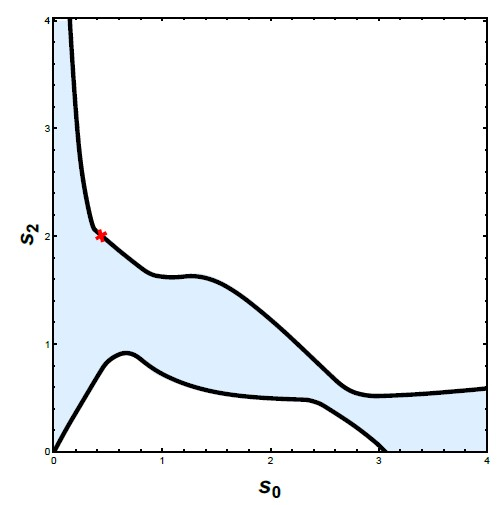
\includegraphics[width=9cm]{11.jpg}
  \caption{River with a red cross marking on-loop $\chi PT$ Adler zeroes $(0.437, 2.003)$ lying near the upper bank. From \cite{7}}
  \label{fig:1}
\end{figure}
In contrast to Lake which excluded very little, these additional constraints rule out a much larger area.













\subsubsection{Effect of Positivity Conditions}
We saw how positivity at $(0,4)$ gave D-wave inequalities. One important point to note is that small changes in $s$ from the point where positivity is imposed must be analytic. This is true for $(0,4)$ but not for points like $(-4, 4), (4, 0), (0, 0)$ and $(4, 4)$ as can be seen in fig.
\begin{figure}[H]
  \centering
  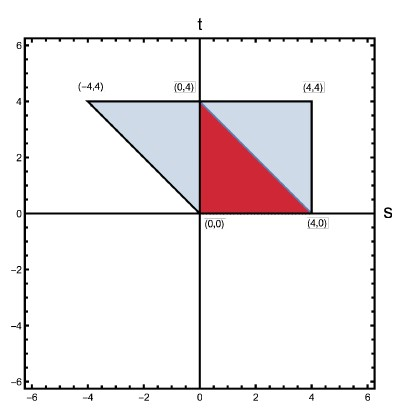
\includegraphics[width=7cm]{12.jpg}
  \caption{Mandelstram Plane. From \cite{7}}
  \label{fig:1}
\end{figure}
So positivity is imposed close to the four points and this causes the banks to slightly recede near the upper "kink" and middle of lower boundary \cite{7}.
\begin{figure}[H]
  \centering
  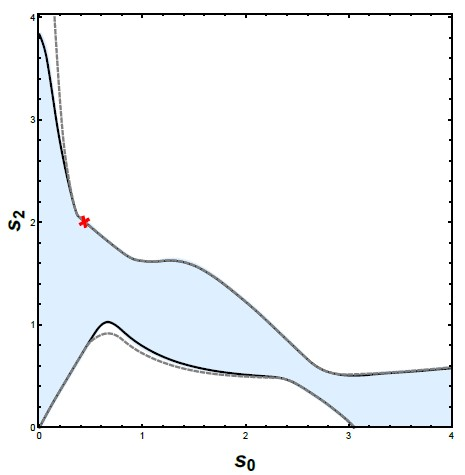
\includegraphics[width=9cm]{13.jpg}
  \caption{From \cite{7}}
  \label{fig:1}
\end{figure}













\section{String Bootstrap}
Two charged scalars exchange massless gravitons between them in $t$ and $u$ (not in $s$ as two charged scalars can't annhilate into a neutral particle) to give \cite{8}
$$
T(s, t, u) \equiv s^{4} A(s, t, u)=-8 \pi G_{N}\left(\frac{s^{2}}{t}+\frac{s^{2}}{u}\right)+\ldots
$$
The first Wilson coefficient is at $\mathcal{O}(s^{0})$
$$
\frac{T(s, t, u)}{8 \pi G_{N}}=s^{4}\left(\frac{1}{s t u}+\alpha \ell_{P}^{6}+O(s)\right)
$$
Using the constraining factor, we want to see what values $\alpha$ using principles involved in S-matrix bootstrap. To do this we need to come up with an ansatz for massless exchange (Impose $s+t+u=0$) compatible with Lorentz invariance (must only involve Mandelstram variables) and crossing ($T(s,t,u)$ is symmetric in all its arguments). Consider
$$
\frac{T}{8 \pi G_{N}}=s^{4}\left(\frac{1}{s t u}+\prod_{A=s, t, u}\left(\rho_{A}+1\right)^{2} \sum_{a+b+c \leq N}^{\prime} \alpha_{(a b c)} \rho_{s}^{a} \rho_{t}^{b} \rho_{u}^{c}\right)
$$
The factor $\prod_{A=s, t, u}\left(\rho_{A}+1\right)^{2} \sim \frac{1}{s t u}$ keeps that part of the ansatz in control at high energies.
$$
\rho_{s} = \frac{\sqrt{s_{0}}-\sqrt{-s}}{\sqrt{s_{0}}+\sqrt{-s}}
$$
maps Mandelstram plane minus the cut to a unit disk. The partial wave relation is given in terms of the $d$-dim version of Legendre polynomials which can be written in terms of Gegenbauer polynomials which are accessed through GegenbauerC in Mathematica.
$$
P_{l}^{(d)}(x)=\frac{l ! \Gamma\left(\frac{d-2}{2}\right)}{4(4 \pi)^{d / 2} \Gamma(d+l-2)} C_{l}^{\frac{d-2}{2}}(x)
$$
$$
P_{l}^{(9)}(x)=\frac{l ! \Gamma\left(\frac{7}{2}\right)}{4(4 \pi)^{9 / 2} \Gamma(7+l)} C_{l}^{7/2}(x)
$$
Using
$$
C_{\ell}^{7/2}(1)=\frac{\Gamma(7+l)}{\Gamma(7)\Gamma(l+1)}
$$
$$
P_{l}^{(9)}(x)=\frac{ \Gamma\left(\frac{7}{2}\right)}{4(4 \pi)^{9 / 2} 6!} \frac{C_{l}^{7/2}(x)}{C_{l}^{7/2}(1)}=\frac{\frac{5}{2}\cdot\frac{3}{2}\cdot\frac{1}{2}\cdot\sqrt{\pi}}{4(4 \pi)^{9 / 2} 5\cdot3\cdot1\cdot6\cdot4\cdot2} \frac{C_{l}^{7/2}(x)}{C_{l}^{7/2}(1)}
$$
$$
P_{l}^{(9)}(x)=\frac{1}{3\cdot 2^{18}\cdot \pi^{4}} \frac{C_{l}^{7/2}(x)}{C_{l}^{7/2}(1)}
$$
Since for massless case,
$$
S_{\ell}(s)=1+\left.i s^{\frac{d-3}{2}} \int_{-1}^{1} d x\left(1-x^{2}\right)^{\frac{d-3}{2}} P_{\ell}^{(d)}(x) \mathcal{T}(s, t)\right|_{t \rightarrow \frac{1}{2}(s-4)(x-1)}
$$
For $d=9$ (9+1 dim),
$$
S_{\ell}(s)=1+\frac{i}{3 \cdot 2^{18} \pi^{4}} s^{3} \int_{-1}^{1} d x\left(1-x^{2}\right)^{3} \frac{C_{\ell}^{7 / 2}(x)}{C_{\ell}^{7 / 2}(1)} \mathcal{T}(s, x)
$$
$$
\begin{aligned}
S_{\ell}(s)=1+\frac{8\pi i G_{N}}{3 \cdot 2^{18} \pi^{4}} s^{7} \int_{-1}^{1} d x&\left(1-x^{2}\right)^{3} \frac{C_{\ell}^{7 / 2}(x)}{C_{\ell}^{7 / 2}(1)}\\
&\left(\frac{4}{s^{3}(1-x^{2})}+\prod_{A=s, t, u}\left(\rho_{A}+1\right)^{2} \sum_{a+b+c \leq N}^{\prime} \alpha_{(a b c)} \rho_{s}^{a} \rho_{t}^{b} \rho_{u}^{c}\right)
\end{aligned}
$$
The way to evaluate this for the ansatz is detailed in Appendix C and the $\frac{1}{stu}$ term is evaluated using NIntegrate. Note that we are working with $\ell_{P}=1$ and $8 \pi G_{N}=64 \pi^{7} \ell_{P}^{8}$. And using that one can use SDPB to impose\\\\
1. $\left|S_{\ell}(s)\right|^{2} \leq 1$\textbf{ for even} $\ell=0,2,..., L$\\\\
Unitarity was imposed on a grid of points given by
$$
\rho\left(s_{k}\right)=e^{i \frac{\pi}{2}\left(1+\cos \frac{\pi k}{n_{\mathrm{pts}}+1}\right)}, \quad k=1,2,..., n_{\mathrm{pts}}
$$
with $n_{\mathrm{pts}}=1000$.\\
We also impose \\\\
2. $\operatorname{Im} T(s, t=0) \geq 0$ \textbf{at all grid points}\\\\
which follows from unitarity. But is useful to impose since unitarity is imposed only for a grid of points and truncated in $N$ and $L$.\\
3. \textbf{For large $\ell$, we impose unitarity as}
$$
1-\operatorname{Re} S_{\ell}(s) \propto \sum_{a b c}^{\prime} \alpha_{(a b c)}(b+1) \operatorname{Im} \rho_{s}^{a} \rho_{-s}^{c} \geq 0
$$
since $\left| S_{\ell}(s)\right|^{2}\leq 1 \Rightarrow \operatorname{Re} S_{\ell}(s)\leq 1$.\\\\
NOTE:- Since Mathematica incorrectly evaluates Imaginary part of objects like $\rho$ by using the wrong branch cut, in numerics where imaginary part is required and its sign is important (like in the above constraints 2 and 3), we use conjugates of those objects to correct for this.\\\\
We also need to impose unitarity at large energies because of the factors of $s$ sitting outside the integral.
\subsection{Large Energy Unitarity}
There is a factor of $s^{4}$ from the ansatz and a factor of $s^{3}$ from the expression of $S_{\ell}$ for $d=9+1$, a total of $s^{7}$ and there needs to a decay of atleast as fast as $\frac{1}{s^{7}}$ in the rest of the expression to keep modulus of partial waves less than 1. The integral is of the form 
$$
I_{\ell}^{a b c}(s)=\rho^{a}(s) \int_{-1}^{1} \mu_{\ell}^{(10)}(x) \rho(t(s, x))^{b} \rho(u(s, x))^{c} d x
$$
where
$$
\mu_{\ell}^{(10)}(x)=\left(1-x^{2}\right)^{3} \frac{C_{\ell}^{(7 / 2)}(x)}{C_{\ell}^{(7 / 2)}(1)}
$$
For even $\ell$ we can use $x \rightarrow -x$ from $-1$ to $0$ and get
$$
I_{\ell}^{a b c}(s)=\rho^{a}(s) \int_{0}^{1}\left(\rho(t)^{b} \rho(u)^{c}+\rho(t)^{c} \rho(u)^{b}\right) \mu_{\ell}^{(10)}(x) d x
$$
Expanding $\mu_{\ell}^{(10)}(x)$ in $(1-x)$ with minimum power being $3$ because of the factor $(1-x^{2})^{3}$ and maximum power of $6+l$ since $(1-x^{2})^{3}$ gives $x^{6}$ and $C_{\ell}^{(7 / 2)}(x)$ gives $x^{\ell}$
$$
\mu_{\ell}^{(10)}(x)=\sum_{n=3}^{6+\ell} \mu_{n}^{\ell}(1-x)^{n}
$$
Our goal boils down to calculating the integral
$$
J_{n}^{b c}(s)=\int_{0}^{1} \rho(t)^{b} \rho(u)^{c}(1-x)^{n} d x
$$
Taking $s_{0}=1$ for simplicity (can easily with few modifications be done for $s_{0}=0.7$),
$$
\begin{array}{l}
\rho(t)=\dfrac{1-\sqrt{\frac{s}{2}(1-x)}}{1+\sqrt{\frac{s}{2}(1-x)}} = \dfrac{\sqrt{\frac{1}{s(1-x)}}-\sqrt{\frac{1}{2}}}{\sqrt{\frac{1}{s(1-x)}}+\sqrt{\frac{1}{2}}}\\
\rho(u)=\dfrac{1-\sqrt{\frac{s}{2}(1+x)}}{1+\sqrt{\frac{s}{2}(1+x)}} = \dfrac{\sqrt{\frac{1}{s(1+x)}}-\sqrt{\frac{1}{2}}}{\sqrt{\frac{1}{s(1+x)}}+\sqrt{\frac{1}{2}}} \\\\
\rho(t)=-1+\ldots .\text{series in }\frac{1}{\sqrt{s(1-x)}}\\
\rho(u)=-1+\ldots .\text{series in }\frac{1}{\sqrt{s(1+x)}}
\end{array}
$$
Since we need to only look at the terms that go to zero slower than $\frac{1}{s^{7}}$ because of the ones that die off faster will vanish at $\infty$. So $J_{n}^{b c}(s)$ with $n\geq 7$ will have $(1-x)^{7}$ which will only appear at $\mathcal{O}(s^{-8})$ onwards due to $\rho(u)$ being a series in $\frac{1}{\sqrt{s(1-x)}}$ and hence can be integrated without worrying about singularities. Since $n\geq 3$, the first term appears at $\mathcal{O}(s^{-4})$.\\\\
For $J_{n}^{b c}(s)$ with $(1-x)^{n}$ and at $\mathcal{O}(s^{-m})$ which in worst case comes all from $\rho_{t}$ in which case we have $(1-x)^{-m}$. Since integral of $(1-x)^{n-m}$ is divergent only if $n-m<-\frac{1}{2}$.\\\\
These integrals can be calculated to be of the following form as explained in the following sections.
$$
I_{\ell}^{a b c}=\sum_{i=0}^{14} g_{i}^{\ell}(a, b, c) \frac{1}{s^{i / 2}}+\sum_{i=8}^{14} h_{i}^{\ell}(a, b, c) \frac{\log (s)}{s^{i / 2}}+\mathcal{O}\left(s^{-15 / 2}\right)
$$
Now for unitarity, we need to impose \textbf{for all $\ell$}\\\\
4. \textbf{All $\dfrac{\log (s)}{s^{i / 2}}$ h-terms to vanish}\\\\
5. \textbf{All  $s^{-i / 2}$ g-terms upto $i=13$ to vanish}\\\\
6. \textbf{14th term $g_{14}$ which goes as $s^{-7}$ goes to a constant at $\infty$ and this needs to be bounded to respect unitarity}

















\subsubsection{Example of $b=c=1$, $n=0$}
Even though this case has $n=0<3$ and doesn't appear in the problem but can be used to understand steps involved. We have
$$
j(s)=\int_{0}^{1} d x \rho(t(s, x)) \rho(u(s, x)) .
$$
At large $s$,
$$
\rho_{t} \rho_{u} \simeq 1-\frac{2 \sqrt{2}(\sqrt{1-x}+\sqrt{1+x})}{\sqrt{s\left(1-x^{2}\right)}}+\frac{8\left(1+\sqrt{1-x^{2}}\right)}{s\left(1-x^{2}\right)}+\mathcal{O}(s^{-3/2})
$$
We divide the integral using an arbitrary cut-off $\delta$ which we will get rid of in the end.
$$
j(s)=\underbrace{\int_{0}^{1-\delta} \rho_{t} \rho_{u} d x}_{\text {outer }}+\underbrace{\int_{1-\delta}^{1} \rho_{t} \rho_{u} d x}_{\text {inner }}
$$
$$
\int_{0}^{1-\delta} \frac{1+\sqrt{1-x^{2}}}{1-x^{2}} d x=\sin^{-1}(1-\delta) + \frac{1}{2} \log \left( -1+\frac{2}{\delta} \right)
$$
$$
\tanh^{-1}(1-\delta)=\frac{1}{2} \log \left( \frac{1+(1-\delta)}{1+(1+\delta)} \right)=\frac{1}{2} \log \left( -1+\frac{2}{\delta} \right)
$$
$$
\frac{8}{s}\int_{0}^{1-\delta} \frac{1+\sqrt{1-x^{2}}}{1-x^{2}} d x=\frac{8}{s}\left(\sin^{-1}(1-\delta) +\tanh^{-1}(1-\delta)\right)
$$
$$
-\frac{2\sqrt{2}}{\sqrt{s}}\int_{0}^{1-\delta} \frac{\sqrt{1-x}+\sqrt{1+x}}{\sqrt{1-x^{2}}} d x=-\frac{2\sqrt{2}}{\sqrt{s}}2\left(\sqrt{2-\delta}-\sqrt{\delta}\right)=4\sqrt{\frac{2}{s}}\left(\sqrt{\delta}-\sqrt{2-\delta}\right)
$$
Putting it all together,
$$
\text { outer } \simeq  1-\delta+4 \sqrt{\frac{2}{s}}(\sqrt{\delta}-\sqrt{2-\delta}) + \frac{8}{s}\left(\sin^{-1}(1-\delta) +\tanh^{-1}(1-\delta)\right)
$$
Now to calculate $\int_{1-\delta}^{1} \rho_{t} \rho_{u} d x$, we make a change of variables to $x=1-\frac{2 \epsilon^{2}}{s}$ and get
$$
\begin{array}{l}
\rho(t)=\dfrac{1-\epsilon}{1+\epsilon}\\
\rho(u)=\dfrac{1-\sqrt{s-\epsilon^{2}}}{1+\sqrt{s-\epsilon^{2}}}\simeq -1 \qquad \text{for high } s
\end{array}
$$
$$
\text { inner } \simeq \frac{4}{s} \int_{0}^{\Delta} \frac{1-\epsilon}{1+\epsilon} \epsilon d \epsilon=\frac{2}{s}[\Delta(\Delta-4)-4 \log (1+\Delta)]
$$
with $\Delta=\sqrt{\frac{\delta s}{2}}$. Expanding for large $\Delta$ (large $s$),
$$
\text { inner } \simeq \delta-4 \sqrt{\frac{2 \delta}{s}}+\frac{4}{s} \log \frac{\delta s}{2}
$$
(There were quite a few typos in the above steps in \cite{7}.)
$$
\frac{8}{s}\tanh^{-1}(1-\delta)=\frac{4}{s} \log \left(\frac{(2-\delta)s}{2} \right)-\frac{4}{s}\log \left(\frac{\delta s}{2} \right)
$$
$$
\begin{aligned}
\text { outer + inner } &\simeq  1-\delta+4 \sqrt{\frac{2\delta}{s}}-4 \sqrt{\frac{2(2-\delta)}{s}} + \frac{8}{s}\sin^{-1}(1-\delta) +\frac{4}{s} \log \left(\frac{(2-\delta)s}{2} \right)\\
&-\frac{4}{s}\log \left(\frac{\delta s}{2} \right)+\delta-4 \sqrt{\frac{2 \delta}{s}}+\frac{4}{s} \log\left( \frac{\delta s}{2}\right)
\end{aligned}
$$
All the terms that might cause trouble for $\delta \rightarrow 0$ get cancelled and now we can take that limit to get
$$
j(s) \simeq 1-\frac{8}{\sqrt{s}}+\frac{4}{s} \log s+\frac{4 \pi}{s}
$$
We see that there are powers of $s$ and also some terms with $\log s$ along with powers of $s$. 













\subsubsection{Evaluation of $J_{n}^{b c}(s)$}
$$
J_{n}^{b c}(s)=\left(\int_{0}^{1-\delta}+\int_{1-\delta}^{1}\right) \rho_{t(s, x)}^{b} \rho_{u(s, x)}^{c}(1-x)^{n} d x
$$
Outer part is evaluated in the same way as in the simple example. Inner part is done by the same change of variables to $x=1-\frac{2 \epsilon^{2}}{s}$
$$
\begin{array}{l}
\rho(t)=\dfrac{1-\epsilon}{1+\epsilon}=\rho_{-\epsilon^{2}}\\
\rho(u)=\dfrac{1-\sqrt{s-\epsilon^{2}}}{1+\sqrt{s-\epsilon^{2}}}=\rho_{-s+\epsilon^{2}}
\end{array}
$$
and
$$
\int_{1-\delta}^{1} \rho_{t}^{b} \rho_{u}^{c}(1-x)^{n} d x=\frac{2^{n+2}}{s^{n+1}} \int_{0}^{\Delta}\left(\rho_{-\epsilon^{2}}\right)^{b}\left(\rho_{-s+\epsilon^{2}}\right)^{c} \epsilon^{2 n+1} d \epsilon
$$
For $n \geq 3$, this integral will contribute at order $\mathcal{O}\left(s^{-4}\right)$ onwards. $\left(\rho_{-s+\epsilon^{2}}\right)^{c}$ can be expanded for large $s$ in $\epsilon$. Now it suffices to calculate 
$$
\mathcal{J}_{\alpha}^{b}=\int_{0}^{\Delta} \rho_{-\epsilon^{2}}^{b} \epsilon^{\alpha} d \epsilon=\int_{0}^{\Delta}\left(\frac{1-\epsilon}{1+\epsilon}\right)^{b} \epsilon^{\alpha} d \epsilon
$$
This can be done by using a generating function
$$
\sum_{b=0}^{\infty} \mathcal{J}_{\alpha}^{b} \eta^{b} =\int_{0}^{\Delta} \frac{\epsilon^{\alpha} d \epsilon}{1-\eta \frac{1-\epsilon}{1+\epsilon}}
=\frac{\Delta^{\alpha+1}}{\alpha+1} \frac{\eta-1-2 \eta_{2} F_{1}\left(1, \alpha+1, \alpha+2, \Delta \frac{\eta+1}{\eta-1}\right)}{\eta^{2}-1} 
$$
and expanding for larde $\Delta$ and exracting $b^{\text{th}}$ coeffiicient. Adding inner and outer bits makes all cutoffs to drop off in limit $\delta \rightarrow 0$ to give something of the form
$$
J_{n}^{b c}(s)=\sum_{j=0}^{14} \frac{e_{j}^{n}(b, c)+\log (s) f_{j}^{n}(b, c)}{s^{j / 2}}+\mathcal{O}\left(s^{-15 / 2}\right)
$$














\subsection{Eliminition of parameters due to $s+t+u=0$}
Putting 
$$
s=-\frac{s_{0} \left(1-\rho _s\right){}^2}{\left(\rho _s+1\right){}^2}
$$
and the corresponding expressions for $t$ and $u$ in $s+t+u=0$ and since crossing symmetry makes $\mathcal{T}$ symmetric in all arguments, we define a symmetrized $\rho^{(a, b,c)}=\rho_{s}^{a} \rho_{t}^{b} \rho_{u}^{c}+$ permutations and the on-shell condition in terms of these is found to be
$$
\begin{aligned}
3\rho^{(2,2,2)}+2\rho^{(2,2,1)}+3\rho^{(2,2,0)}-4\rho^{(2,1,1)}-24\rho^{(1,1,1)}&\\
+2\rho^{(2,1,0)}-4\rho^{(1,1,0)}+3\rho^{(2,0,0)}+2\rho^{(1,0,0)}+3\rho^{(0,0,0)}&=0
\end{aligned}
$$
Using this we can eliminate $\alpha_{(2,2,2)}$.\\\\
And noting that
$$
\rho^{(a,b,c)}\rho^{(d,e,f)}=(..)\rho^{(a+d,b+e,c+f)}+(..)\rho^{(a+e,b+f,c+d)}+(..)\rho^{(a+e,b+d,c+f)}+\ldots
$$
we can multiply the on-shell condition by $\rho^{(a,b,c)}$ and eliminate $\alpha_{(a+2,b+2,c+2)}$ which has sum of indices $= N+6$ for $a+b+c=N$. So if number of coefficients (after symmetrizations) is $f(N)$ then by multipling each one of them to the on-shell condition we can eliminate $f(N)$ elements out of the $f(N+6)$ elements six rows below as shown in red in fig.
\begin{figure}[H]
  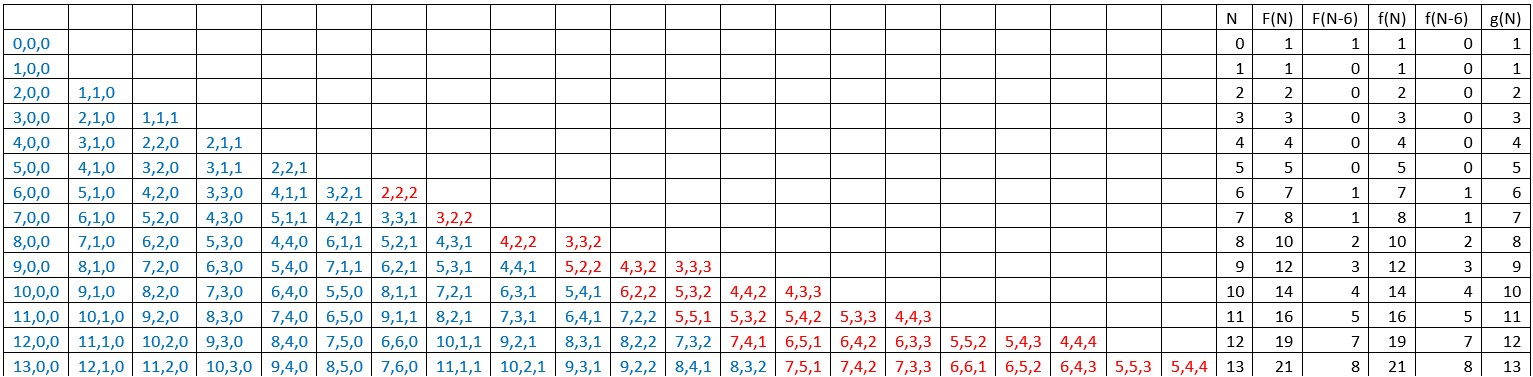
\includegraphics[width=\linewidth]{14.jpg}
  \caption{Eliminated coefficients in red}
  \label{fig:1}
\end{figure}
So, initially number of coeffiecients is $f(N)$ and then after $f(N-6)$ eliminations, it becomes $g(N)=f(N)-f(N-6)$ with $f(N)$ for negative $N$ defined as $0$. We find that
$$
f(N)=F(N)=\frac{N^{2}}{12}+\frac{N}{2}+\frac{(-1)^{N}}{8}+\frac{2}{9} \cos \left(\frac{2 \pi N}{3}\right)+\frac{47}{72}
$$
and 
$$
F(N)-F(N-6)=N
$$
We see that for negative values of $-5,...,-1$, $F(N-6)=0=f(N-6)$ but for $-6$, $F(N-6)=1\neq 0=f(N-6)$. So we can write apart from $g(0)=1$, $g(N)=N$ for $N>0$.So total number of parameters for $N_{max}$ is $1+\frac{N_{max}(N_{max}+1)}{2}$ which for $N_{max}=13$ is $92$.















\subsection{Dispersion relation at fixed $t$ for $\alpha$}
Defining 
$$
\left.g(z) \equiv \frac{T(s, t)}{8 \pi G_{N} s^{4}}\right|_{s=-t / 2+z}=\frac{1}{t\left(\frac{t}{2}+z\right)\left(\frac{t}{2}-z\right)}+\alpha+\ldots
$$
Since $T(s,t)$ has cuts for $s=-t/2+z>0$ and $s+t=t/2 +z<0$ in complex $s$-plane at fixed $t$, $g(z)$ will have cuts for $z<-t/2$ and $z>t/2$ in complex $Z$-plane. $g\left(z^{*}\right)=[g(z)]^{*}$ and crossing symmetry implies that $g(z)=g(-z)$. We can also take $g(z)\rightarrow 0$ at $|z|\rightarrow \infty$ which is a weaker than assumption that $T(s, t) / s^{2} \rightarrow 0$ when $|s| \rightarrow \infty$ which is usually used.
\begin{figure}[H]
  \centering
  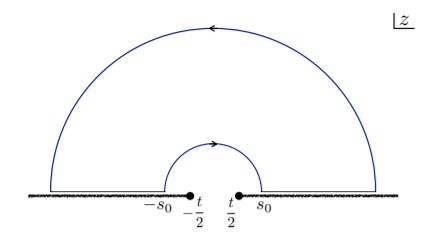
\includegraphics[width=7cm]{15.jpg}
  \caption{From \cite{8}}
  \label{fig:1}
\end{figure}
We perform contour integration with function $\frac{g(z)}{z}$ with contours as shown in figure. The contribution of semi-circular contour at $\infty$ vanishes because $g(z)\rightarrow 0$ at $|z|\rightarrow \infty$. So we get,
$$
\begin{aligned}
\int_{0}^{\pi} d (s_{0} e^{i \theta}) \frac{g(s_{0} e^{i \theta})}{s_{0} e^{i \theta})} = i \int_{0}^{\pi} d \theta g(s_{0} e^{i \theta}) &=\int_{s_{0}}^{\infty} \frac{d z}{z}[g(z+i \epsilon)-g(-z+i \epsilon)] \\ &=2 i \int_{s_{0}}^{\infty} \frac{d z}{z} \operatorname{Im} g(z+i \epsilon) 
\end{aligned}
$$
In limit $0<|t/2|<s_{0} \rightarrow 0$, we have
$$
i \int_{0}^{\pi} d \theta g(s_{0} e^{i \theta})=i \int_{0}^{\pi} d \theta\left[\frac{1}{t\left(\frac{t}{2}+z\right)\left(\frac{t}{2}-z\right)}+\alpha+\ldots\right]_{z=s_{0} e^{i \theta}} \rightarrow i \pi \alpha
$$
since 
$$
\int_{0}^{\pi} d \theta\left[\frac{1}{t\left(\frac{t}{2}+z\right)\left(\frac{t}{2}-z\right)}\right]_{z=s_{0} e^{i \theta}} =\int_{0}^{\pi} d \theta\left[\frac{1}{t\left(\frac{t^{2}}{4}-s_{0}^{2} e^{2i \theta}\right)}\right]
$$
Taking $|t|\rightarrow 0$ first, we see that the integral oscillates to zero leaving only the $\alpha$ term.
$$
\int_{0}^{\pi} d \theta\left[\frac{1}{t\left(\frac{t^{2}}{4}-s_{0}^{2} e^{2i \theta}\right)}\right]\simeq -\int_{0}^{\pi} d \theta\left[\frac{e^{-2i \theta}}{t s_{0}^{2} }\right]\simeq 0
$$
And for $s_{0}\rightarrow 0$,
$$
2 i \int_{s_{0}}^{\infty} \frac{d z}{z} \operatorname{Im} g(z+i \epsilon) =\frac{2 i}{8 \pi G_{N}} \int_{0}^{\infty} \frac{d s}{s^{5}} \operatorname{Im} T(s+i \epsilon, t=0)
$$
With $8 \pi G_{N}=64 \pi^{7}$,
$$
\alpha=\int_{0}^{\infty} ds\ \frac{\operatorname{Im} T(s+i \epsilon, t=0)}{32 \pi^{8} s^{5}}
$$
And using optical theorem, we can write $\operatorname{Im} T(s+i \epsilon, t=0)\geq 0 \Rightarrow \alpha \geq 0$










\subsection{Minimizing $\alpha$}
All of the constraints mentioned are linear in parameters and hence can be written in a form $\sum_{n=0}^{N} z_{n} W_{j}^{n}(x) \succeq 0 \quad$ for all $x \geq 0$ and $1 \leq j \leq J$ but we need $\alpha$ also in terms of the parameters. We have for $\ell_{P}=1$
$$
\frac{T(s, t, u)}{8 \pi G_{N}}=s^{4}\left(\frac{1}{s t u}+\alpha +O(s)\right)
$$
and
$$
\frac{T}{8 \pi G_{N}}=s^{4}\left(\frac{1}{s t u}+\prod_{A=s, t, u}\left(\rho_{A}+1\right)^{2} \sum_{a+b+c \leq N}^{\prime} \alpha_{(a b c)} \rho_{s}^{a} \rho_{t}^{b} \rho_{u}^{c}\right)
$$
So we need to pick out the term independent of $s$ in 
$$
\prod_{A=s, t, u}\left(\rho_{A}+1\right)^{2} \sum_{a+b+c \leq N}^{\prime} \alpha_{(a b c)} \rho_{s}^{a} \rho_{t}^{b} \rho_{u}^{c}
$$
We have 
$$
\begin{array}{l}
\rho(s)=\dfrac{1-\sqrt{-\frac{s}{s_{0}}}}{1+\sqrt{-\frac{s}{s_{0}}}} =1+\mathcal{O}(\sqrt{s})\\
\rho(t)=\dfrac{1-\sqrt{\frac{s}{2s_{0}}(1-x)}}{1+\sqrt{\frac{s}{2s_{0}}(1-x)}} =1+\mathcal{O}(\sqrt{s})\\
\rho(u)=\dfrac{1-\sqrt{\frac{s}{2s_{0}}(1+x)}}{1+\sqrt{\frac{s}{2s_{0}}(1+x)}} =1+\mathcal{O}(\sqrt{s})
\end{array}
$$
So,
$$
\alpha=64 \sum_{a+b+c \leq N}^{\prime} \alpha_{(a b c)} 
$$
But these are not our parameters. We need to work with the symmetrized paramters which are coeficients to $\rho^{(a, b,c)}=\rho_{s}^{a} \rho_{t}^{b} \rho_{u}^{c}+$ permutations. We can write using fact that $\rho_{s,t,u}=1$ at $\mathcal{O}(s^{0})$,
$$
\sum_{a+b+c \leq N}^{\prime} \alpha^{sym}_{(a b c)} \rho^{(a, b,c)}=\sum_{a+b+c \leq N}^{\prime} \alpha^{sym}_{(a b c)} \left(\rho_{s}^{a} \rho_{t}^{b} \rho_{u}^{c}+\ldots \right)=\sum_{a+b+c \leq N}^{\prime} \alpha^{sym}_{(a b c)} N_{per}(a,b,c)
$$
where $ N_{per}(a,b,c)$ is the number of permutations of triplet $(a,b,c)$, for example it is $1$ for ${(1,1,1)}$, $6$ for ${(1,2,3), (1,3,2), (2,1,3), (2,3,1), (3,1,2), (3,2,1)}$ etc.. And the unsymmetrized expression gives
$$
\sum_{a+b+c \leq N}^{\prime} \alpha_{(a b c)} \rho_{s}^{a} \rho_{t}^{b} \rho_{u}^{c}=\sum_{a+b+c \leq N}^{\prime} \alpha_{(a b c)}
$$
Since $L.H.S$ of the two are equal by definition of the new symmetrized coefficients, we have
$$
\alpha=64 \sum_{a+b+c \leq N}^{\prime} N_{per}(a,b,c) \alpha^{sym}_{(a b c)} 
$$
which is linear in terms of the parameters and can be put into SDPB.\\\\
To minimize $\alpha$ we maximize $-\alpha$.\\\\
For $N_{max}=13$ and $L_{max}=28$, the value obtained was $\alpha_{min}=3.62$ while the authors of \cite{8} obtained $\alpha_{min}=4.87$. Unlike 3D bootstrap which converges for a fixed $N_{max}$ at $L_{max}=N_{max}+1$, in string bootstrap the values of $L_{max}$ needed are much higher for example for $N=13$, $L\simeq 70$ and for $N=24$, $L\simeq 200$. Also the convergence as $N$ increases is exponential decay to $\alpha_{min}=0.13\pm 0.02$ and hence is very sensitive. Moreover the authors of \cite{8} used $s_{0}=0.713..$ and at an $(N,L)$ far from convergence, this might be the most probable reason for the mismatch. Higher $(N,L)$ computations are very time consuming and we will be working on it in the future.
















\section{Bounds on Wilson Coefficient Ratios}
This section follows discussion in \cite{9} and \cite{10}.














\subsection{Crossing-Symmetric Dispersion Relation}
$2\rightarrow 2$ scattering can be described by Mandelstram variable $s,t,u$. The way we have used dispersion relations so far with fixed $t$ in complex $s$-plane is not crossing symmetric. These follow $s+t+u=\mu=4m^{2}$. Defining shifted variables $s_{1}=s-\frac{\mu}{3}, s_{2}=t-\frac{\mu}{3}, s_{3}=u-\frac{\mu}{3}$ and $s_{1}+s_{2}+s_{3}=0$. Crossing symmetry means $\mathcal{M}\left(s_{1}, s_{2}\right)=\mathcal{M}\left(s_{2}, s_{3}\right)=\mathcal{M}\left(s_{3}, s_{1}\right)$. Branch cuts for $s,t,u\geq 4m^{2}=\mu$ become $s_{1},s_{2},s_{3}\geq \frac{8m^{2}}{3}=\frac{2\mu}{3}$. To make $s_{1},s_{2},s_{3}$ lie on a cubic hypersurface $\left(s_{1}(z)-a\right)\left(s_{2}(z)-a\right)\left(s_{3}(z)-a\right)=-a^{3}$, we parametrize them as follows
$$
s_{k}=a-\frac{a\left(z-z_{k}\right)^{3}}{z^{3}-1}, \quad k=1,2,3
$$
$z_{k}$ are cube roots of unity so that
$$
\left(s_{1}(z)-a\right)\left(s_{2}(z)-a\right)\left(s_{3}(z)-a\right)=-\frac{a^{3}\left(z-z_{1}\right)^{3}\left(z-z_{2}\right)^{3}\left(z-z_{3}\right)^{3}}{(z^{3}-1)^{3}}=-a^{3}
$$
as required. We restrict $a$ to $-\frac{\mu}{3} \leq a<\frac{2 \mu}{3}$. We also define $x=-\left( s_{1} s_{2} + s_{2} s_{3} + s_{3} s_{1} \right)=\frac{-27 a^{2} z^{3}}{\left(z^{3}-1\right)^{2}}, \quad y=-s_{1} s_{2}s_{3}=\frac{-27 a^{3} z^{3}}{\left(z^{3}-1\right)^{2}}$ and  $a=\frac{y}{x}=\frac{s_{1} s_{2}s_{3}}{\left( s_{1} s_{2} + s_{2} s_{3} + s_{3} s_{1} \right)}$. And one can write amplitude in terms of $(z,a)$ as 
$$
\overline{\mathcal{M}}(z, a)=\mathcal{M}\left(s_{1}, s_{2}\right)
$$
Now to see where the branch cuts are in $(z,a)$, we look at $s_{1}>\frac{2\mu}{3}$ with $s_{1} \in \mathbb{R}$. For $s_{1} \in \mathbb{R}$, (and noting that in general $a\neq 0$ and $z\neq -1,0,1$),
$$
\begin{aligned}
\operatorname{Im}\left(1-\dfrac{(z-1)^{3}}{z^{3}-1}\right)&=0 \\
\operatorname{Im}\left(\dfrac{z^{3}-3 z^{2}+3 z-1}{z^{3}-1}\right)&=0 \\
\operatorname{Im}\left(\dfrac{z(z-1)}{z^{3}-1}\right)&=0 \\
\operatorname{Im}\left(\dfrac{z^{2}+z+1}{z}\right)&=0 \qquad \text{if $z$ is real, so is $1/z$}\\
\operatorname{Im}(z+1)+\operatorname{Im}\left(\dfrac{1}{z}\right)=\operatorname{Im}(z)+\operatorname{Im}\left(\dfrac{1}{z}\right)&=0 \\
\text{Using }\operatorname{Im}(\dfrac{1}{z})&=-\dfrac{1}{|z|^{2}}\operatorname{Im}(z)\\
\Rightarrow |z|=1 \qquad & \text{ OR } \qquad \operatorname{Im}(z)=0
\end{aligned}
$$
For $-\frac{2\mu}{9}<a<0$, the cuts map to unit circle in $z$-plane ($|z|=1$)
\begin{figure}[H]
  \centering
  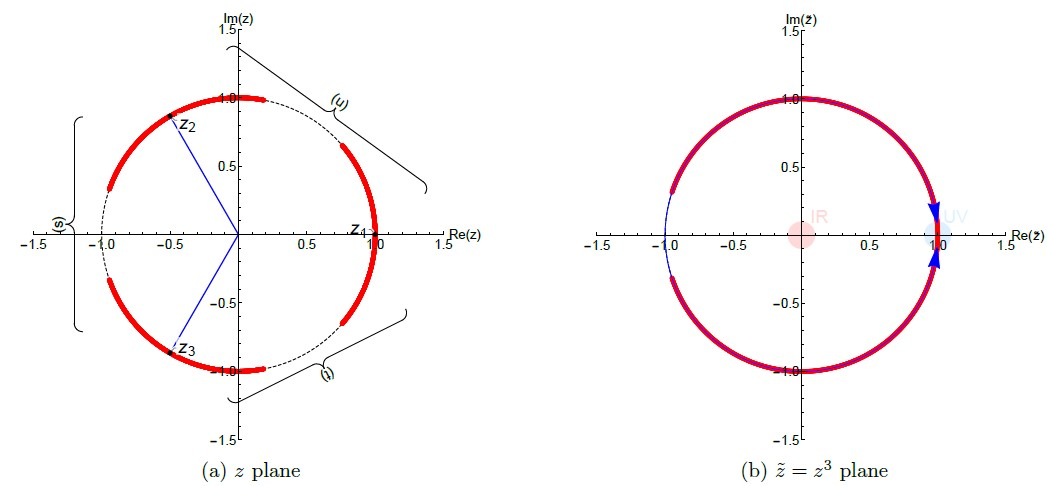
\includegraphics[width=\linewidth]{16.jpg}
  \caption{Cuts in $z$-plane and $\tilde z (=z^{3})$-plane. From \cite{10}}
  \label{fig:1}
\end{figure}
Defining $\tilde z (=z^{3})$, we can write the following completely symmetric dispersion relation using fixed $a$.
$$
\mathcal{M}(\tilde{z}, a)=\alpha_{0}+\frac{1}{\pi} \int_{\frac{2 \mu}{3}}^{\infty} \frac{d s_{1}^{\prime}}{s_{1}^{\prime}} \mathcal{A}\left(s_{1}^{\prime} ; s_{2}^{(+)}\left(s_{1}^{\prime}, a\right)\right) H\left(s_{1}^{\prime}, \tilde{z}\right)
$$
where 
$$
\mathcal{A}_{1}\left(s_{1}, s_{2}\right) \equiv \lim _{\epsilon \rightarrow 0} \frac{1}{2 i}\left[\mathcal{M}\left(s_{1}+i \epsilon, s_{2}\right)-\mathcal{M}\left(s_{1}-i \epsilon, s_{2}\right)\right], \quad s \geqslant 2 \mu / 3
$$
which is the s-channel discontinuity and $\alpha_{0}=$ $\mathcal{M}(z=0, a)$ and
$$
\begin{aligned}
&H\left(s_{1}^{\prime}, \tilde{z}\right)=\frac{27 a^{2} \tilde{z}\left(2 s_{1}^{\prime}-3 a\right)}{27 a^{3} \tilde{z}-27 a^{2} \tilde{z} s_{1}^{\prime}-(1-\tilde{z})^{2}\left(s_{1}^{\prime}\right)^{3}} \\
&s_{2}^{(+)}\left(s_{1}^{\prime}, a\right)=-\frac{s_{1}^{\prime}}{2}\left[1-\left(\frac{s_{1}^{\prime}+3 a}{s_{1}^{\prime}-a}\right)^{1 / 2}\right]
\end{aligned}
$$















\subsection{Univalence and de Branges' Theorem}
Univalence of a function $f$ implies $f(z)=f(w) \Rightarrow z=w$ OR $z\neq w \Rightarrow f(z)\neq f(w)$ in a domain $\mathbb{D}$. And local univalence at $z=z_{0} \Rightarrow f^{\prime}\left(z_{0}\right) \neq 0$. Global univalence of course implies local univalence $\forall z_{0} \in \mathbb{D}$. This is very constraining. For example, consider $g(z)=az+b z^{2}+c$ and consider its univalence in unit disk $\mathbb{D}=\{ z\left| |z|<1 \right. \}$. $g(z)-g(w)=az+b z^{2} -aw-b w^{2}=a(z-w)(1+\frac{b}{a}(z+w))$. For $g(z)=g(w)$ to imply necessarily that $z=w$, $|1+\frac{a}{b}(z+w)|\neq 0 \quad \forall |z|<1$. This happens if $|\frac{a}{b}|<\frac{1}{2}$. Noticing that univalence $f(z)=\dfrac{g(z)-g(0)}{g^{\prime}(0)}$ is equivalent to univalence of $g(z)$ (both are related by what is called an affine transformation), we define a class of univalent functions called Schlicht functions which has expansion of the form
$$
f(z)=z+\sum_{p=2}^{\infty} b_{p} z^{p}, \quad|z|<1
$$
with $f(0)=0, f^{\prime}(0)=1$\\\\
An example of this kind of function is the Koebe Function.
$$
k(z)=\frac{z}{(1-z)^{2}}=z+\sum_{p=2}^{\infty} p z^{p}
$$
A useful concept of Grunsky inequalities gives a necessary and sufficient conditions for a Schlicht function with unit disk domain. Grunsky coefficients are defined for a function $f$ as follows
$$
\ln \frac{f(t)-f(z)}{t-z}=\sum_{j, k=0}^{\infty} \omega_{j, k} t^{j} z^{k}
$$
where $\omega_{j, k}$ are the Grunsky coefficients. \\
A useful property is that a Mobius transformation of a function $f$ also has common Grunsky coefficients for $\forall j,k\geq 1$. To see this consider $h$, a Mobius transformation of $f$,
$$
h(z)=\frac{a f(z)+b}{c f(z)+d}, \qquad a d-b c \neq 0
$$
$$
\frac{h(t)-h(z)}{t-z}=\frac{\frac{a f(t)+b}{c f(t)+d}-\frac{a f(z)+b}{c f(z)+d}}{t-z}=(ad-bc)\frac{1}{(c f(t)+d)(c f(z)+d)}\frac{f(t)-f(z)}{t-z}
$$
Taking logarithm on both sides,
$$
\ln \frac{h(t)-h(z)}{t-z}=\ln (ad-bc)-\ln (c f(t)+d)-\ln (c f(z)+d)+ \ln \frac{f(t)-f(z)}{t-z}
$$
For $ad-bc\neq 0$, $\ln (ad-bc)$ is just a constant and contributes only to $\omega_{0,0}$ and since $\ln (c f(t)+d)$ is a function of $t$ alone it contributes only to $\omega_{j, 0}$ and $\ln (c f(z)+d)$ is a function of $z$ alone and contributes to $\omega_{0, k}$, and hence these dont contribute to $\omega_{j, k}$ for $j,k\geq 1$. So,
$$
\widetilde{\omega}_{j, k}=\omega_{j, k}, \qquad \forall j, k \geq 1 
$$
\textbf{Theorem 1:- }$f$ is a Schlicht function iff 
$$
\left|\sum_{j, k=1}^{N} \omega_{j, k} \lambda_{j} \lambda_{k}\right| \leq \sum_{k=1}^{N} \frac{1}{k}\left|\lambda_{k}\right|^{2}, \qquad \forall N\in \mathbb{N} \text{ and } \lambda_{k}, k=1, \ldots, N
$$
For Koebe function,
$$
\begin{aligned}
\ln \left( \frac{\frac{t}{(1-t)^{2}}-\frac{z}{(1-z)^{2}}}{t-z}\right)&=\ln \left( \frac{t+z^{2}t-2zt-z-zt^{2}+2tz}{(t-z)(1-t)^{2}(1-z)^{2}}\right)\\
&=\ln \left( \frac{1-zt}{(1-t)^{2}(1-z)^{2}}\right)\\
&=\ln(1-zt)-2\ln(1-t)-2\ln(1-z)
\end{aligned}
$$
Since $\ln (1-x)=-\sum_{n=1}^{\infty} \frac{x^{n}}{n}=-x-\frac{x^{2}}{2}-\frac{x^{3}}{3}-\cdots$, the Grunsky coefficients are $\omega_{j, 0}=\omega_{0, j}=$ $2 / j \text{ and } \omega_{j, k}=-\delta_{j, k} / j$.\\\\
\textbf{Theorem 2 (de Branges' theorem):- }If $f$ is a Schlicht function with $f(z)=z+\sum_{p=2}^{\infty} b_{p} z^{p}, \quad|z|<1$, then its coefficients satisfy
$$
\left|b_{n}\right| \leq n, \quad \forall n \geq 2
$$
Equality is iff $f$ is a Koebe function or its "rotation" defined as follows
$$
f(z)=e^{-i \theta} k\left(e^{i \theta} z\right), \quad \forall \theta \in \mathbb{R}
$$



































\subsection{Deriving Bounds on Wilson Coefficients}
$\mathcal{M}$, when written in terms of $s_{1}, s_{2}$, can be expanded in  $x=-\left( s_{1} s_{2} + s_{2} s_{3} + s_{3} s_{1} \right) \text{ and } y=-s_{1} s_{2}s_{3},$
$$
\mathcal{M}\left(s_{1}, s_{2}\right)=\sum_{p,q=0}^{\infty} W_{p, q} x^{p} y^{q}
$$
And $\mathcal{M}(\tilde{z}, a)$ can be expanded about $\tilde z=0$ as follows
$$
\mathcal{M}(\tilde{z}, a)=\sum_{n=0}^{\infty} \alpha_{n}(a) a^{2 n} \tilde{z}^{n}
$$
Using the transformation, one can write $\alpha_{n}(a) a^{2 n}$ as
$$
\alpha_{p}(a) a^{2 p}=\sum_{n=0}^{p} \sum_{m=0}^{n} W_{n-m, m} a^{m}(-1)^{p-n}(-27)^{n} a^{2 n}\left(\begin{array}{c}
-2 n \\
p-n
\end{array}\right)
$$
And the kernel $H\left(s_{1}^{\prime}, \tilde{z}\right)$ can be expanded about $\tilde z=0$ as
$$
H\left(s_{1}^{\prime}, \tilde{z}\right)=\sum_{n=0}^{\infty} \beta_{n}\left(a, s_{1}^{\prime}\right) \tilde{z}^{n}
$$
The expression obtained \cite{10} is involved but the following can be deduced from it
$$
\begin{aligned}
\beta_{0}\left(a, s_{1}\right)&=0\\
\beta_{1}\left(a, s_{1}\right)&=\frac{27 a^{2}}{s_{1}^{3}}\left(3 a-2 s_{1}\right)
\end{aligned}
$$
Physically allowed domains are $a\in [-2 \mu / 9,2 \mu / 3)$ and $s_{1} \in [2 \mu / 3, \infty)$. For $\beta_{1}\left(a, s_{1}\right) \neq 0$, we need $3a\leq 2s_{1}=\frac{4\mu}{3} \Rightarrow a\leq \frac{4\mu}{9}$
$$
a \in\left(-\frac{2 \mu}{9}, 0\right) \cup\left(0, \frac{4 \mu}{9}\right) 
$$
and in this case
$$
\beta_{1}\left(a, s_{1}\right)<0
$$
One can write
$$
a^{2 n} \alpha_{n}(a)=\frac{1}{\pi} \int_{\frac{2 \mu}{3}}^{\infty} \frac{d s_{1}^{\prime}}{s_{1}^{\prime}} \mathcal{A}\left(s_{1}^{\prime} ; s_{2}^{(+)}\left(s_{1}^{\prime}, a\right)\right) \beta_{n}\left(a, s_{1}^{\prime}\right) \quad n>0
$$
Using $a_{\ell}$, the partial wave element of imaginary part of the amplitude (the discontinuity), 
$$
\mathcal{A}\left(s_{1} ; s_{2}^{(+)}\left(s_{1}, a\right)\right) =\Phi\left(s_{1} ; \alpha\right) \sum_{\ell=0}^{\infty}(2 \ell+2 \alpha) a_{\ell}\left(s_{1}\right) C_{\ell}^{(\alpha)}\left(\sqrt{\xi\left(s_{1}, a\right)}\right) 
$$
where
$$
\begin{aligned}
\xi\left(s_{1}, a\right) &=\left(1+\frac{2 s_{2}^{+}\left(s_{1}, a\right)+\frac{2 \mu}{3}}{s_{1}-\frac{2 \mu}{3}}\right)^{2}=\xi_{0}+4 \xi_{0}\left(\frac{a}{s_{1}-a}\right)\\
\xi_{0}&=\frac{s_{1}^{2}}{\left(s_{1}-2 \mu / 3\right)^{2}}
\end{aligned}
$$
$\xi_{0}=\frac{s_{1}^{2}}{\left(s_{1}-2 \mu / 3\right)^{2}}>0$ when $s_{1} \in\left[\frac{2 \mu}{3}, \infty\right)$ and additionally $s_{1}>a \Rightarrow a \in\left(-\frac{2 \mu}{9}, \frac{2 \mu}{3}\right)$ will make $\xi\left(s_{1}, a\right)>1 \Rightarrow C_{\ell}^{(\alpha)}\left(\sqrt{\xi\left(s_{1}, a\right)}\right)>0$. Unitarity keeps $a_{\ell}>0$ over $s_{1} \in\left[\frac{2 \mu}{3}, \infty\right)$.\\\\
\textbf{We have $\mathcal{A}\left(s_{1} ; s_{2}^{(+)}\left(s_{1}, a\right)\right)>0$ for $s_{1} \in$ $\left[\frac{2 \mu}{3}, \infty\right)$ and $a \in\left(-\frac{2 \mu}{9}, \frac{2 \mu}{3}\right)$}\\\\
Now defining
 $$
F\left(\tilde{z} ; s_{1}, a\right)=\frac{H\left(\tilde{z} ; s_{1}, a\right)}{\beta_{1}\left(a, s_{1}\right)}=\tilde{z}+\sum_{n=2}^{\infty} \frac{\beta_{n}\left(a, s_{1}\right)}{\beta_{1}\left(a, s_{1}\right)} \tilde{z}^{n}
$$
since $\beta_{0}=0$. Also
$$
F\left(\tilde{z} ; s_{1}, a\right)=\frac{\tilde{z}}{1+\gamma \tilde{z}+\tilde{z}^{2}}\qquad \qquad \text{with }\gamma=27\left(\frac{a}{s_{1}}\right)^{2}\left(1-\frac{a}{s_{1}}\right)-2
$$
For $|\gamma|<2$, there will be no singularities in the unit disc. And $F\left(\tilde{z} ; s_{1}, a\right)$ is defined as long as $\beta_{1}\neq 0$ which holds for $a \in\left(-\frac{2 \mu}{9}, 0\right) \cup\left(0, \frac{4 \mu}{9}\right)$ and $|\gamma|<2$ under these conditions. 
$$
F\left(\tilde{z} ; s_{1}, a\right)=\frac{\tilde{z}}{1-2 \tilde{z}+\tilde{z}^{2}+(\gamma+2) \tilde{z}}=\frac{\tilde{z}}{(1-\tilde{z}^{2})^{2}\left(1+(\gamma+2)\frac{ \tilde{z}}{(1-\tilde{z}^{2})^{2}}\right)}
$$
$$
F\left(\tilde{z} ; s_{1}, a\right)=k(\tilde{z})\left(1-\frac{27 a^{2}\left(a-s_{1}\right)}{s_{1}^{3}} k(\tilde{z})\right)^{-1}
$$
where $k(\tilde{z})$ is the Koebe function 
$$
k(\tilde{z})=\frac{\tilde z}{(1-\tilde{z}^{2})^{2}}
$$
and $F\left(\tilde{z} ; s_{1}, a\right)$ is a Mobius transformation of $k(\tilde{z})$ and hence has the same Grunsky coefficients as the Koebe function $\omega_{p, q}=-\frac{\delta_{p, q}}{p}, \quad p, q \geq 1$ which satisfies the Grunsky inequalities and as a result is a Schlicht function on the unit disc. And since $H\left(\tilde{z} ; s_{1}, a\right)$ is related to it by an affine transormation, it is a univalent function on the unit disc.\\\\
\textbf{$H\left(\tilde{z} ; s_{1}, a\right)$ is a univalent function on the unit disc $|\tilde{z}|<1$ for $a \in\left(-\frac{2 \mu}{9}, 0\right) \cup\left(0, \frac{4 \mu}{9}\right)$ and $s_{1} \in\left[\frac{2 \mu}{3}, \infty\right)$}\\\\
\textbf{Using de Branges' theorem on $F\left(\tilde{z} ; s_{1}, a\right)$, $\left|\dfrac{\beta_{n}\left(a, s_{1}\right)}{\beta_{1}\left(a, s_{1}\right)}\right| \leq n, \quad n \geq 2$ for $a \in\left(-\frac{2 \mu}{9}, 0\right) \cup\left(0, \frac{4 \mu}{9}\right)$ and $s_{1} \in\left[\frac{2 \mu}{3}, \infty\right)$}\\\\
Now we use
$$
a^{2 n} \alpha_{n}(a)=\frac{1}{\pi} \int_{\frac{2 \mu}{3}}^{\infty} \frac{d s_{1}^{\prime}}{s_{1}^{\prime}} \mathcal{A}\left(s_{1}^{\prime} ; s_{2}^{(+)}\left(s_{1}^{\prime}, a\right)\right) \beta_{n}\left(a, s_{1}^{\prime}\right)
$$
for n=1
$$
-\alpha_{1}(a) a^{2}=\frac{1}{\pi} \int_{\frac{2 \mu}{3}}^{\infty} \frac{d s_{1}^{\prime}}{s_{1}^{\prime}} \mathcal{A}\left(s_{1}^{\prime} ; s_{2}^{(+)}\left(s_{1}^{\prime}, a\right)\right)\left[-\beta_{1}\left(a, s_{1}^{\prime}\right)\right]
$$
Using the fact that when $a \in\left(-\frac{2 \mu}{9}, 0\right) \cup\left(0, \frac{4 \mu}{9}\right)$ and $s_{1}^{\prime} \in\left[\frac{2 \mu}{3}, \infty\right)$,  $\mathcal{A}\left(s_{1}^{\prime} ; s_{2}^{(+)}\left(s_{1}^{\prime}, a\right)\right)>0$ and $\beta_{1}\left(a, s_{1}^{\prime}\right)<0$, we have
$$
\alpha_{1}(a)<0, \quad a \in\left(-\frac{2 \mu}{9}, \frac{4 \mu}{9}\right) .
$$
Consider the ratio $|\frac{\alpha_{n}(a) a^{2 n}}{\alpha_{1}(a) a^{2}}|$ which is well defined for the above mentione range of $a$. Now consider the numerator
$$
\begin{aligned}
\left|\alpha_{n}(a) a^{2 n}\right|&=\frac{1}{\pi}\left|\int_{\frac{2 \mu}{3}}^{\infty} \frac{d s_{1}^{\prime}}{s_{1}^{\prime}} \mathcal{A}\left(s_{1}^{\prime} ; s_{2}^{(+)}\left(s_{1}^{\prime}, a\right)\right) \beta_{n}\left(a, s_{1}^{\prime}\right)\right|\\
\text{Triangle inequality}\\
&\leq \frac{1}{\pi} \int_{\frac{2 \mu}{3}}^{\infty} \frac{d s_{1}^{\prime}}{s_{1}^{\prime}}\left|\mathcal{A}\left(s_{1}^{\prime} ; s_{2}^{(+)}\left(s_{1}^{\prime}, a\right)\right) \beta_{n}\left(a, s_{1}^{\prime}\right)\right|\\
\text{$\mathcal{A}\left(s_{1}^{\prime} ; s_{2}^{(+)}\left(s_{1}^{\prime}, a\right)\right)>0$}\\
&=\frac{1}{\pi} \int_{\frac{2 \mu}{3}}^{\infty} \frac{d s_{1}^{\prime}}{s_{1}^{\prime}} \mathcal{A}\left(s_{1}^{\prime} ; s_{2}^{(+)}\left(s_{1}^{\prime}, a\right)\right)\left|\beta_{n}\left(a, s_{1}^{\prime}\right)\right|\\
\text{$\left|\dfrac{\beta_{n}\left(a, s_{1}\right)}{\beta_{1}\left(a, s_{1}\right)}\right| \leq n$}\\
&\leq \frac{1}{\pi} \int_{\frac{2 \mu}{3}}^{\infty} \frac{d s_{1}^{\prime}}{s_{1}^{\prime}} \mathcal{A}\left(s_{1}^{\prime} ; s_{2}^{(+)}\left(s_{1}^{\prime}, a\right)\right) n\left|\beta_{1}\left(a, s_{1}^{\prime}\right)\right|\\
\text{$\beta_{1}\left(a, s_{1}^{\prime}\right)< 0$}\\
&=\frac{n}{\pi} \int_{\frac{2 \mu}{3}}^{\infty} \frac{d s_{1}^{\prime}}{s_{1}^{\prime}}  \mathcal{A}\left(s_{1}^{\prime} ; s_{2}^{(+)}\left(s_{1}^{\prime}, a\right)\right)\left[-\beta_{1}\left(a, s_{1}^{\prime}\right)\right] \\
\text{$\alpha_{1}(a)<0$}\\
&=n\left(-\alpha_{1}(a) a^{2}\right)=n\left|\alpha_{1}(a) a^{2}\right|\\
\end{aligned}
$$
\\\\
\textbf{$\left|\dfrac{\alpha_{n}(a) a^{2 n}}{\alpha_{1}(a) a^{2}}\right| \leq n$ for $n\geq 2$ and $a \in\left(-\frac{2 \mu}{9}, 0\right) \cup\left(0, \frac{4 \mu}{9}\right)$}\\\\
Recalling 
$$
\alpha_{p}(a) a^{2 p}=\sum_{n=0}^{p} \sum_{m=0}^{n} W_{n-m, m} a^{m}(-1)^{p-n}(-27)^{n} a^{2 n}\left(\begin{array}{c}
-2 n \\
p-n
\end{array}\right)
$$
For $p=0$,
$$
\alpha_{0}=W_{0,0}
$$
$p=1$
$$
\alpha_{1}a^{2}=-27 a^2 (a W_{0,1}+W_{1,0})
$$
$p=2$
$$
\alpha_{2}a^{4}=729 a^4 \left(a^2 W_{0,2}+a W_{1,1}+W_{2,0}\right)-54 a^2 (a W_{0,1}+W_{2,0})
$$
$p=3$
$$
\begin{aligned}
\alpha_{3}a^{6}=&-19683 a^6 \left(a^3 W_{0,3}+a^2 W_{1,2}+a W_{2,1}+W_{3,0}\right)+2916 a^4 \left(a^2 W_{0,2}+a W_{1,1}+W_{2,0}\right)\\
&-81 a^2 (a W_{0,1}+W_{1,0})
\end{aligned}
$$
Using these in the above inequality for $n=2$ gives
$$
-2 \leq 2-\frac{27 a^{2}\left(a\left(a W_{0,2}+W_{1,1}\right)+W_{2,0}\right)}{a W_{0,1}+W_{1,0}} \leq 2
$$
and for $n=3$,
$$
-3 \leq 3+\frac{27 a^{2}\left(a\left(-4 a W_{0,2}+27 a\left(a\left(a\left(a W_{0,3}+W_{1,2}\right)+W_{2,1}\right)+W_{3,0}\right)-4 W_{1,1}\right)-4 W_{2,0}\right)}{a W_{0,1}+W_{1,0}} \leq 3
$$
which to be satisfied for range $-\frac{2 \mu}{9}<a<\frac{4 \mu}{9}$ requires denominator to be non-zero 
$$
\Rightarrow \frac{W_{0,1}}{W_{1,0}} \neq -\frac{1}{a} \in \left(-\infty,-\frac{9}{4 \mu} \right) \cup\left(\frac{9}{2 \mu}, \infty \right)
$$
which gives us bound on the ratio $\frac{W_{0,1}}{W_{1,0}}$,
$$
-\frac{9}{4 \mu}<\frac{W_{0,1}}{W_{1,0}}<\frac{9}{2 \mu}
$$
For $\mu=4$,
$$
-\frac{9}{16}<\frac{W_{0,1}}{W_{1,0}}<\frac{9}{8}
$$

















\subsection{Numerical Results}



\subsubsection{Extracting $W_{p,q}$}
An amplitude known in the form $\mathcal{M}(s,x)=\mathcal{M}\left(s_{1}+\frac{4}{3},1+2\left(\dfrac{s_{2}+\frac{4}{3}}{s_{1}-\frac{8}{3}}\right)\right)$ can be expanded in $s_{1}$ and $s_{2}$,
$$
\mathcal{M}\left(s_{1}+\frac{4}{3},1+2\left(\dfrac{s_{2}+\frac{4}{3}}{s_{1}-\frac{8}{3}}\right)\right)=\sum_{a,b=0}^{\infty} \mathcal{C}_{a,b} s_{1}^{a} s_{2}^{b}
$$
Also since $ s_{1} +s_{2} + s_{3}=0$, $x=-\left( s_{1} s_{2} + s_{2} s_{3} + s_{3} s_{1} \right)=s_{1}^{2}+s_{2}^{2}+s_{1}s_{2} \text{ and } y=-s_{1} s_{2}s_{3}=s_{1}s_{2}(s_{1}+s_{2})$, 
$$
\mathcal{M}\left(s_{1}+\frac{4}{3},1+2\left(\dfrac{s_{2}+\frac{4}{3}}{s_{1}-\frac{8}{3}}\right)\right)=\sum_{p,q=0}^{\infty} W_{p, q} x^{p} y^{q}=\sum_{p,q=0}^{\infty} W_{p, q} \left(s_{1}^{2}+s_{2}^{2}+s_{1}s_{2}\right)^{p} \left(s_{1}s_{2}(s_{1}+s_{2}) \right)^{q}
$$
The goal is to find $W_{p, q}$ when $\mathcal{C}_{a,b}$ are known.
$$
\sum_{a,b=0}^{\infty} \mathcal{C}_{a,b} s_{1}^{a} s_{2}^{b}=\sum_{p,q=0}^{\infty} W_{p, q} \left(s_{1}^{2}+s_{2}^{2}+s_{1}s_{2}\right)^{p} \left(s_{1}s_{2}(s_{1}+s_{2}) \right)^{q}
$$
Calling the term $s_{1}^{a}s_{2}^{b}\sim \mathcal{O}(s^{a+b})$, we have $\left(s_{1}^{2}+s_{2}^{2}+s_{1}s_{2}\right)^{p}\sim \mathcal{O}(s^{2p})$ and $ \left(s_{1}s_{2}(s_{1}+s_{2}) \right)^{q} \sim \mathcal{O}(s^{3q})$. This shows that a particular term $s_{1}^{a}s_{2}^{b}$ can appear with multiple coefficients $W_{p, q}$ with $2p+3q=a+b$. So taking the example of $W_{0,2}$, we see $2p+3q=6$. The other $W$(s) that satisfy this is(are) $W_{3,0}$. So one can see the following
$$\begin{aligned}
\sum_{a+b=6} \mathcal{C}_{a,b} s_{1}^{a} s_{2}^{b}=&W_{0, 2}  \left(s_{1}s_{2}(s_{1}+s_{2}) \right)^{2}+W_{3,0} \left(s_{1}^{2}+s_{2}^{2}+s_{1}s_{2}\right)^{3} \\
=&W_{0, 2}  \left(s_{1}^{4} s_{2}^{2}+2 s_{1}^{3} s_{2}^{3}+s_{1}^{2} s_{2}^{4}\right)\\
&+W_{3,0} \left(s_{1}^6 + 3 s_{1}^5 s_{2} + 6 s_{1}^4 s_{2}^2 + 7 s_{1}^3 s_{2}^3 + 6 s_{1}^2 s_{2}^4 +  3 s_{1} s_{2}^5 + s_{2}^6\right) \\
\end{aligned}
$$
Now coefficient of any two of the $s_{1}^{a} s_{2}^{b}$ can give two equations in two variables $W_{0, 2}$ and $W_{3,0}$ which can be solved to obtain the two. Some coefficients like $W_{0, 1} ,W_{2, 1}$ are single with no degeneracies and need only matching of one $s_{1}^{a} s_{2}^{b}$. Some like $\left(W_{0, 3}, W_{3, 1}\right)$ pairs like the example above and triplets like $\left(W_{0, 4}, W_{3, 2}, W_{6, 0}\right)$ need matching of three different $s_{1}^{a} s_{2}^{b}$ and so on.













\subsubsection{For $\pi^{0}\pi^{0}\rightarrow \pi^{0}\pi^{0}$ Scattering}
The SDPB outputs the maximum value of $a \cdot z$ and the value of the parameters i.e. all entries of $\vec{a}$ (here $a_{nm}, b_{nm}$'s) for which it is maximized which can then be used to write $\mathcal{M}(\pi^{0}\pi^{0}\rightarrow \pi^{0}\pi^{0})(s,x)$ corresponding to those parameters and the procedure outlined above can be used to obtain the value of Wilson coefficients for various S-matrices. This was done for boundaries of Lake, River, Peninsula (but with weaker experimental values than in \cite{2}) and for Minimum Averaged Cross Section (explained below).\\\\
For a particular $s_{0},s_{2}$, both Adler zeroes are imposed and the total averaged cross section $<\sigma(s_{0})>=\frac{1}{2 s_{c u t}} \int_{4}^{s_{\text {cut }}} d s \sqrt{\frac{s-4}{s}} \operatorname{Im}\left(M^{A B \rightarrow A B}(s, t=0)\right)$ (setting $s_{cut}=375$) is minimized. Keeping $s_{0}$ and then finding the $s_{2}$ at which this minimum value is minimum and repeating this for some values of $s_{0}$ gives a plot. This particular form of total averaged cross section is ideal since it is linear in the parameters and hence amenable to SDPB implementation. \\\\
The results of the above procedure gives the following values of the ratio $\dfrac{W_{p,q}}{W_{1,0}}$ vs $s_{0}$
\begin{figure}[H]
  \centering
  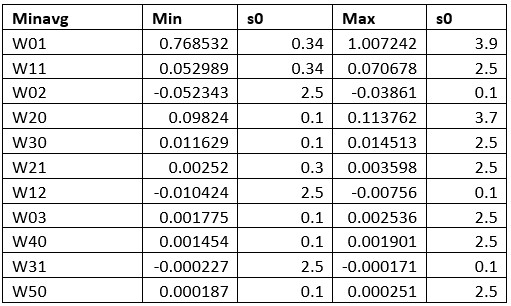
\includegraphics[width=9cm]{TabMinavg.jpg}
  \caption{The values of minimum and maximum values of $W_{p,q}$ among the various points on \textbf{minimum average curve ($N_{max}=14, L_{max}=19$)} and the value of $s_{0}$ where they occur.}
\end{figure}

\begin{figure}[H]
  \centering
  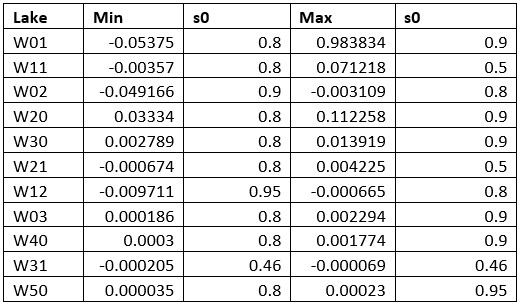
\includegraphics[width=10cm]{TabLake.jpg}
  \caption{The values of minimum and maximum values of $W_{p,q}$ among the various points on \textbf{Lake boundary ($N_{max}=10, L_{max}=11$)} and the value of $s_{0}$ where they occur.}
\end{figure}

\begin{figure}[H]
  \centering
  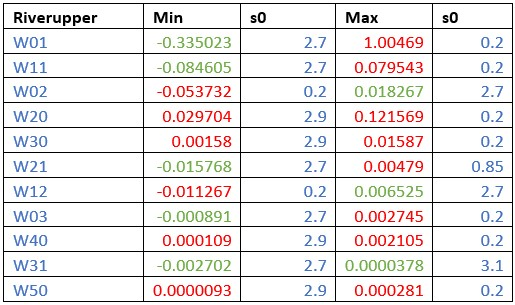
\includegraphics[width=10cm]{TabUp.jpg}
  \caption{The values of minimum and maximum values of $W_{p,q}$ among the various points on \textbf{Upper River boundary ($N_{max}=16, L_{max}=19$)} and the value of $s_{0}$ where they occur.}
\end{figure}

\begin{figure}[H]
  \centering
  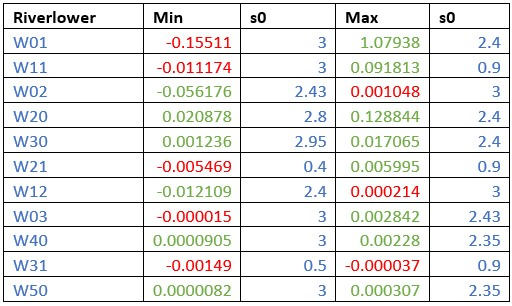
\includegraphics[width=10cm]{TabLow.jpg}
  \caption{The values of minimum and maximum values of $W_{p,q}$ among the various points on \textbf{Lower River boundary ($N_{max}=16, L_{max}=19$)} and the value of $s_{0}$ where they occur.}
\end{figure}
The Green values are the Max/Min in the entire River boundary (Lower+Upper).

\begin{figure}[H]
  \centering
  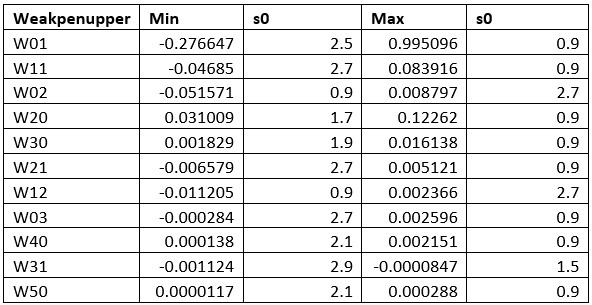
\includegraphics[width=11cm]{TabWPU.jpg}
  \caption{The values of minimum and maximum values of $W_{p,q}$ among the various points on \textbf{Lower Weak Peninsula boundary ($N_{max}=16, L_{max}=19$)} and the value of $s_{0}$ where they occur.}
\end{figure}

\begin{figure}[H]
  \centering
  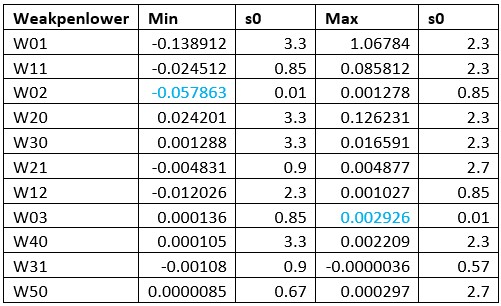
\includegraphics[width=10cm]{TabWPL.jpg}
  \caption{The values of minimum and maximum values of $W_{p,q}$ among the various points on \textbf{Lower Weak Peninsula boundary ($N_{max}=16, L_{max}=19$)} and the value of $s_{0}$ where they occur.}
\end{figure}
The River provides almost all of the overall Min/Max values of Wilson coefficients among the various kinds of boundaries/curves. Two values marked in Blue come from the Lower weak peninsula boundary which are also very close to the corresponding River values. 

\begin{figure}[H]
    \centering
    \subfloat[\centering Overall Max/Min Wilson coefficient values (Green from River and Blue from Lower weak peninsula)]{{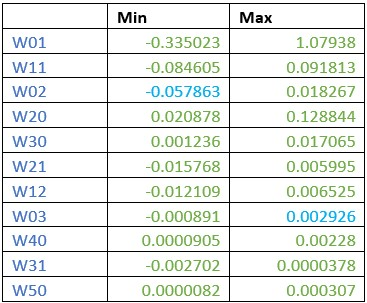
\includegraphics[width=7cm]{TabTot.jpg} }}
    \subfloat[\centering Theoretical bounds]{{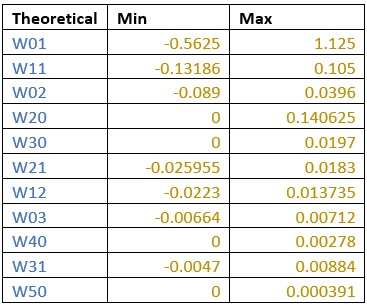
\includegraphics[width=7cm]{TabTh.jpg} }}
     \caption{The numerical values lie within theoretical bounds}
\end{figure}
Since most Max/Min values come from River, the plots for $\dfrac{W_{p,q}}{W_{1,0}}$ vs $s_{0}$ are shown below with the upper and lower bounds plotted as straight lines. One can see that all numerical values lie within the theoretical bounds.
\begin{figure}[H]
    \centering
   {{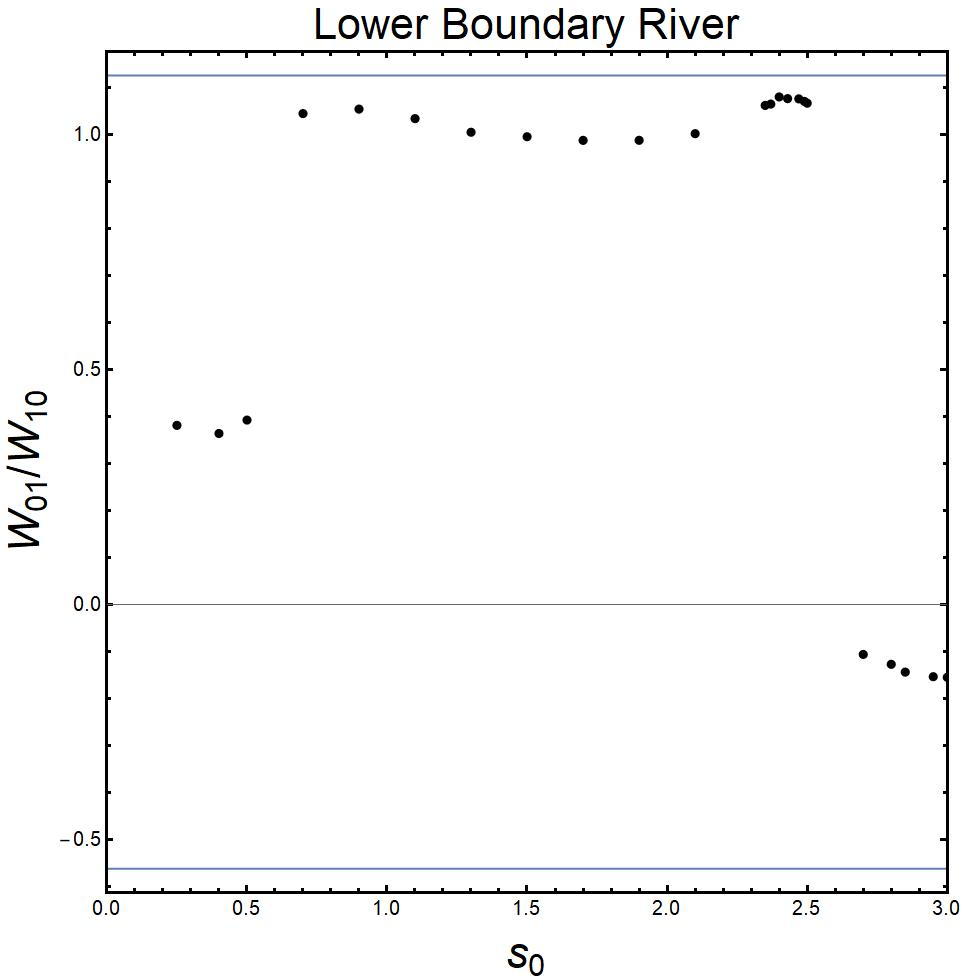
\includegraphics[width=6.7cm]{L01.jpg} }}
  {{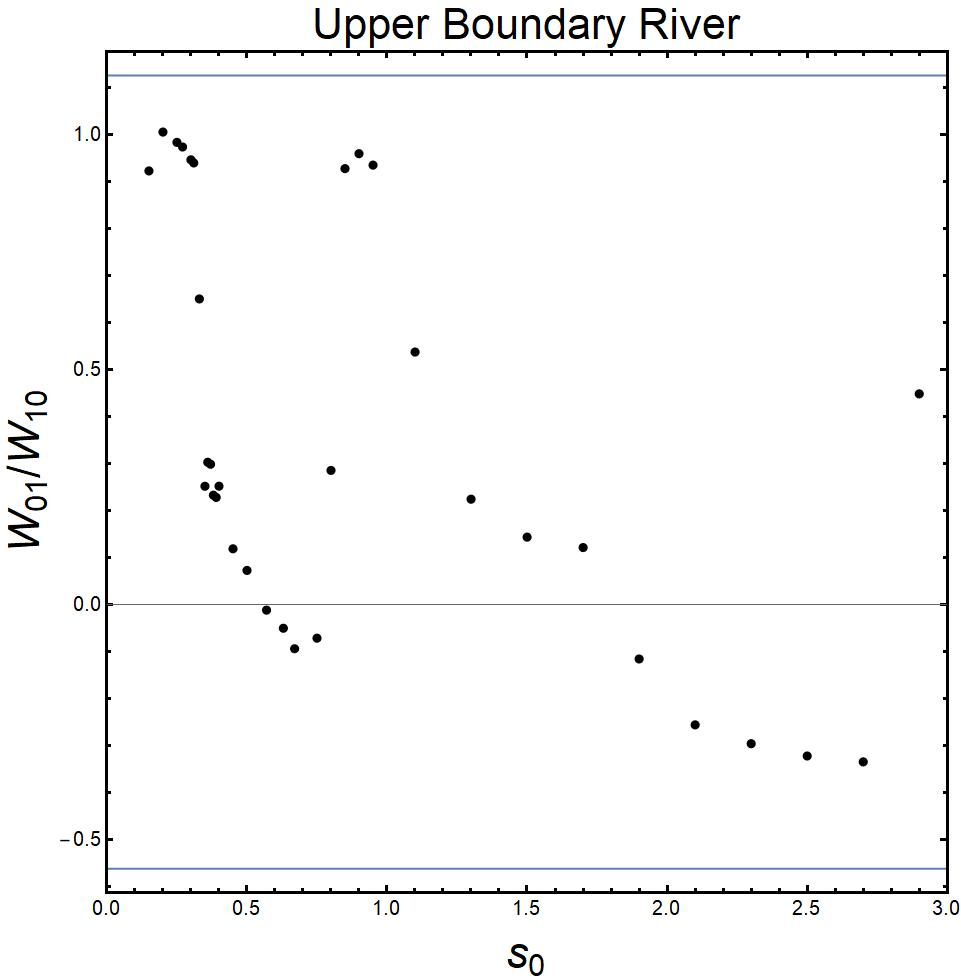
\includegraphics[width=6.7cm]{U01.jpg} }}
\end{figure}

\begin{figure}[H]
    \centering
   {{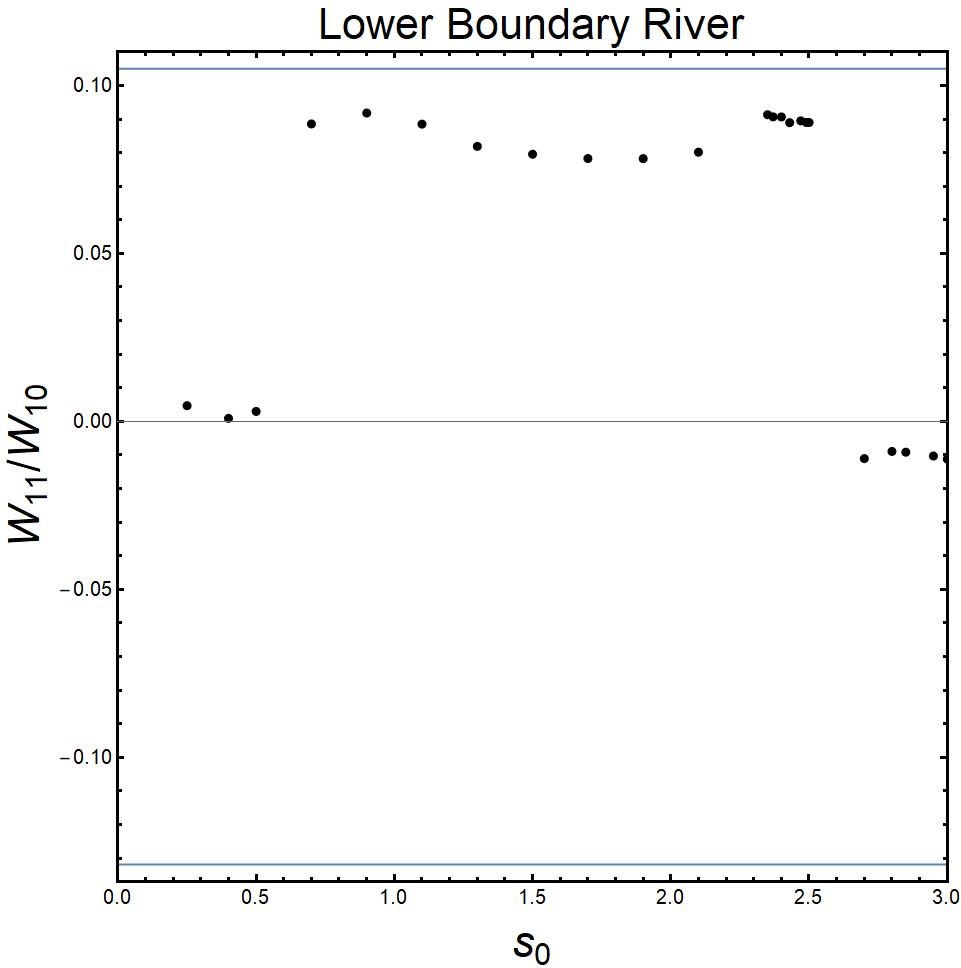
\includegraphics[width=6.7cm]{L11.jpg} }}
  {{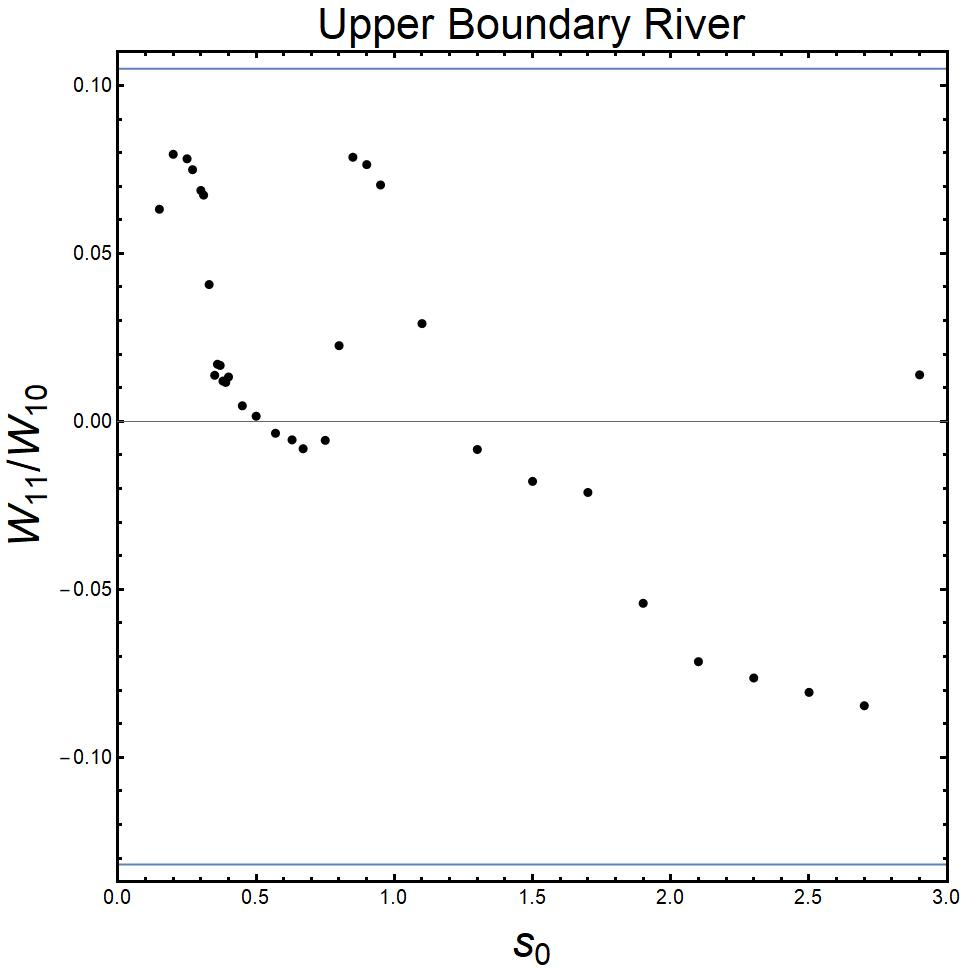
\includegraphics[width=6.7cm]{U11.jpg} }}
\end{figure}

\begin{figure}[H]
    \centering
   {{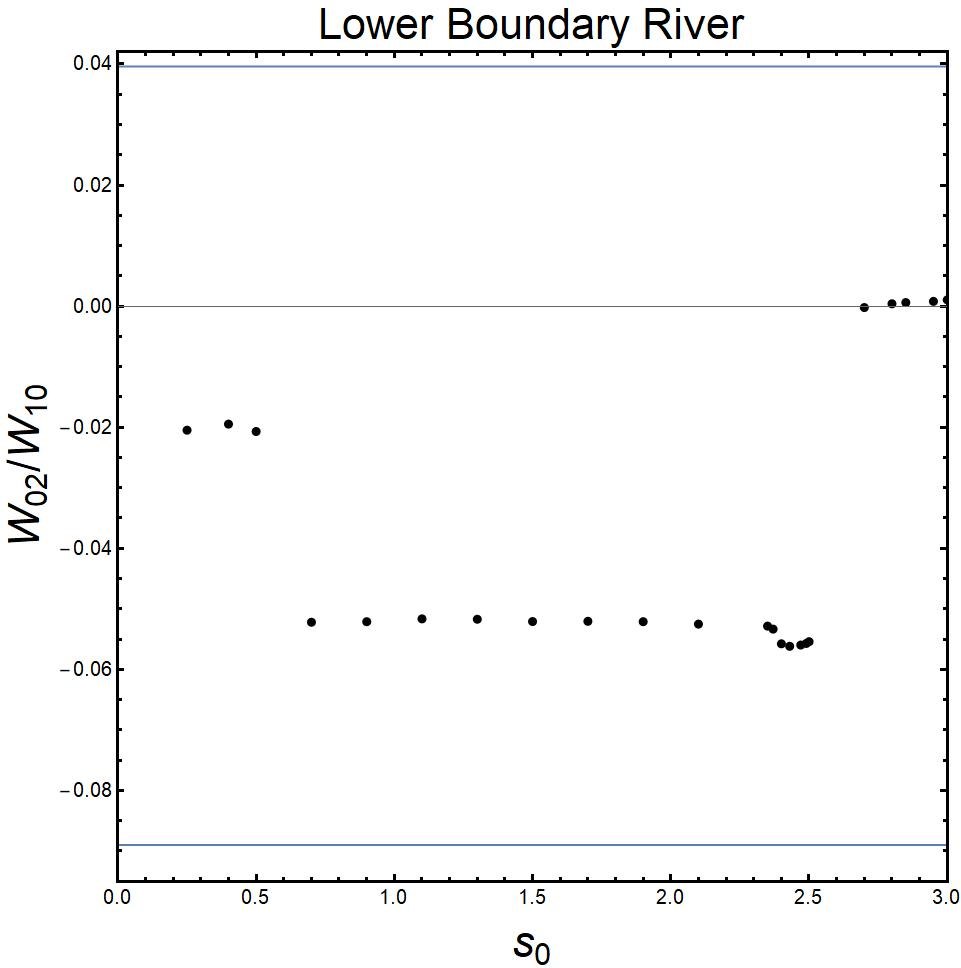
\includegraphics[width=6.7cm]{L02.jpg} }}
  {{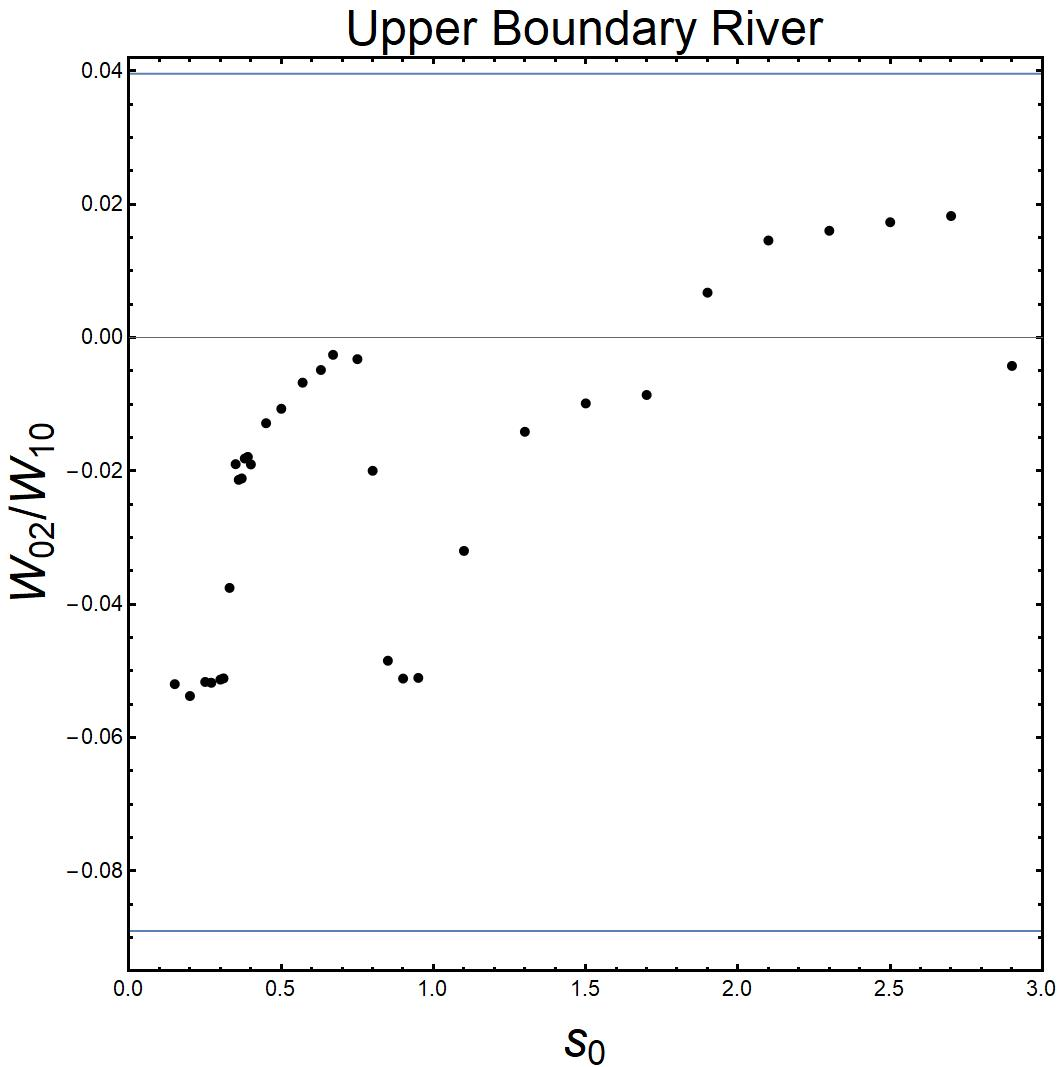
\includegraphics[width=6.7cm]{U02.jpg} }}
\end{figure}

\begin{figure}[H]
    \centering
   {{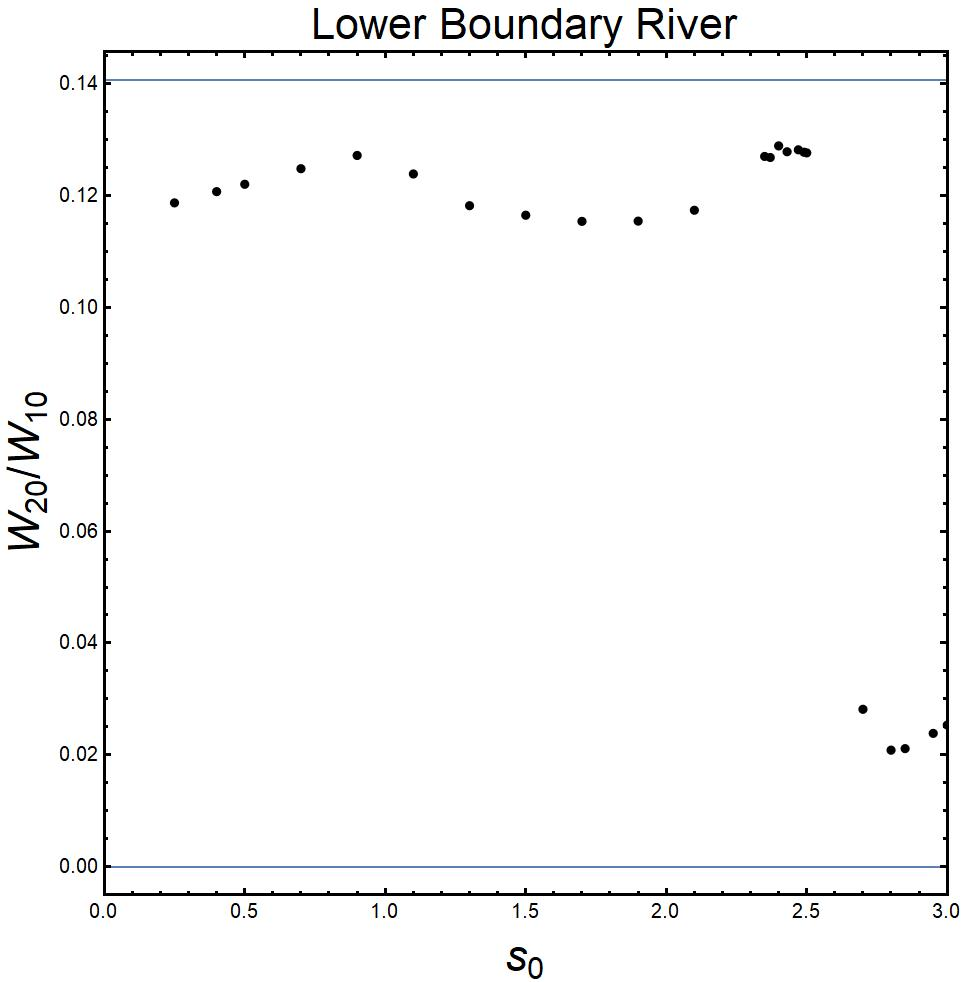
\includegraphics[width=6.7cm]{L20.jpg} }}
  {{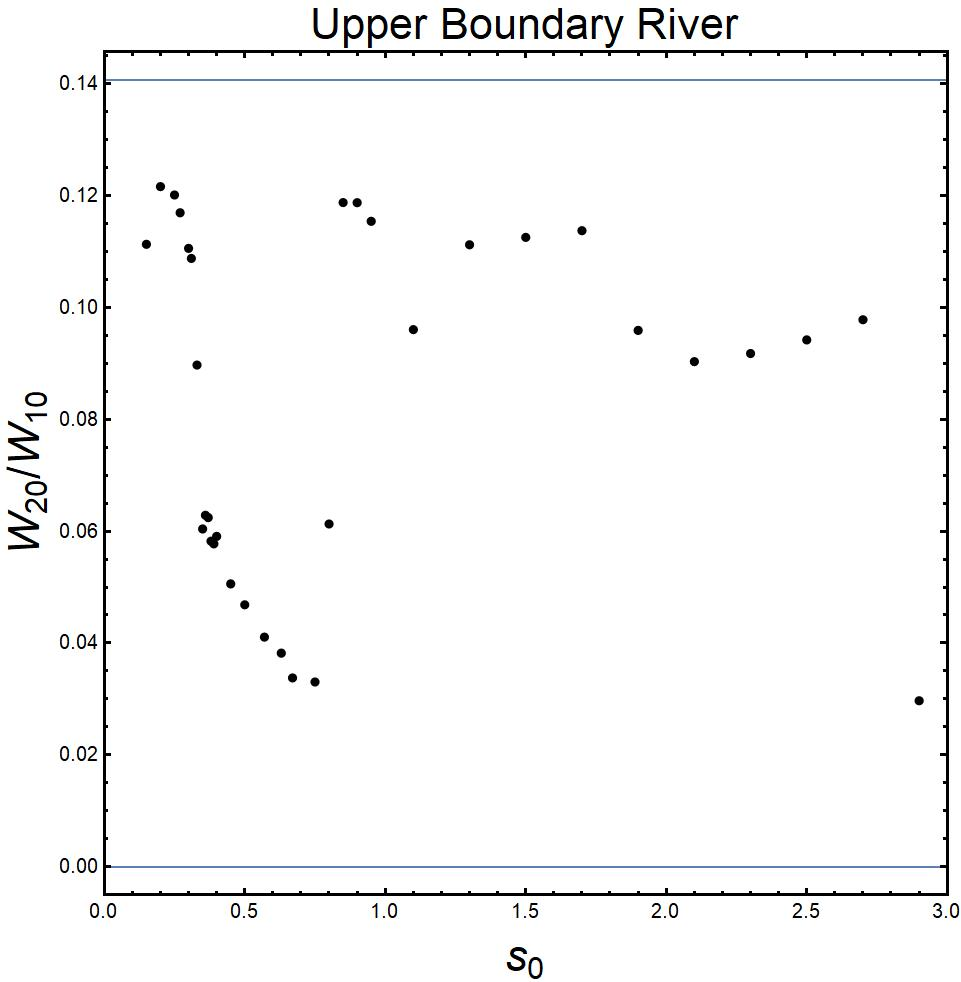
\includegraphics[width=6.7cm]{U20.jpg} }}
\end{figure}

\begin{figure}[H]
    \centering
   {{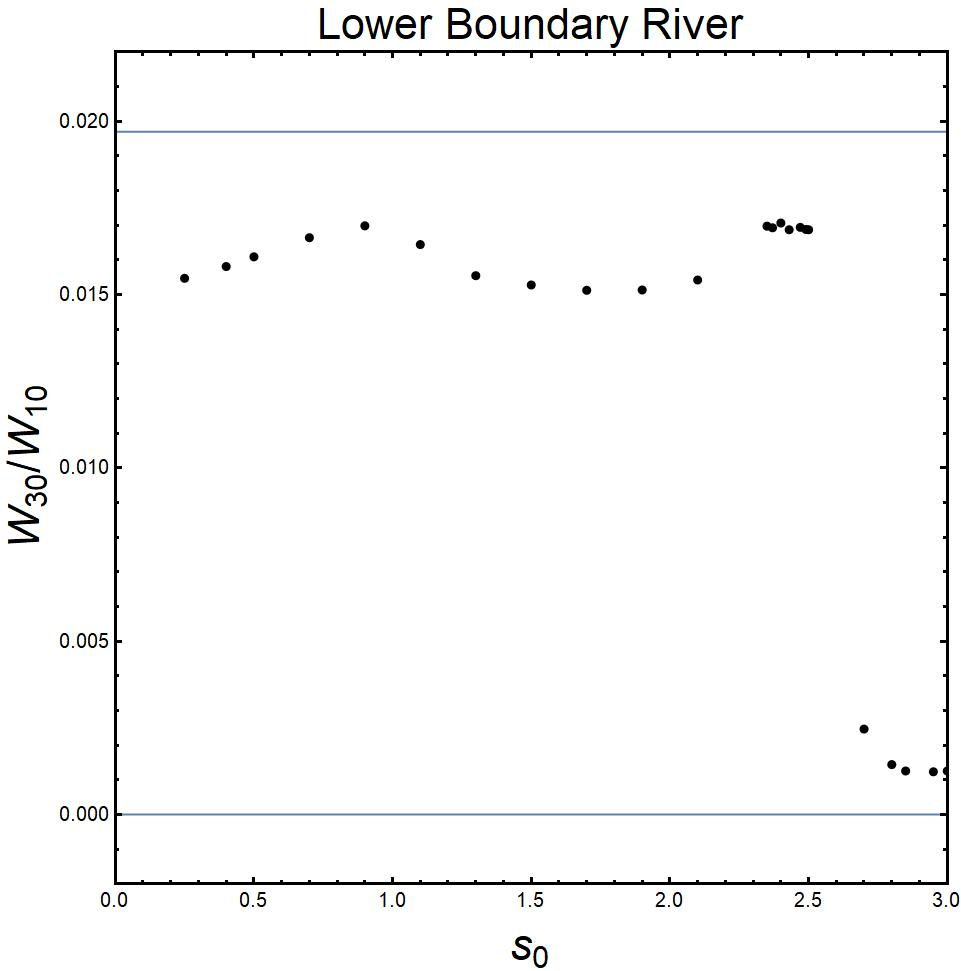
\includegraphics[width=6.7cm]{L30.jpg} }}
  {{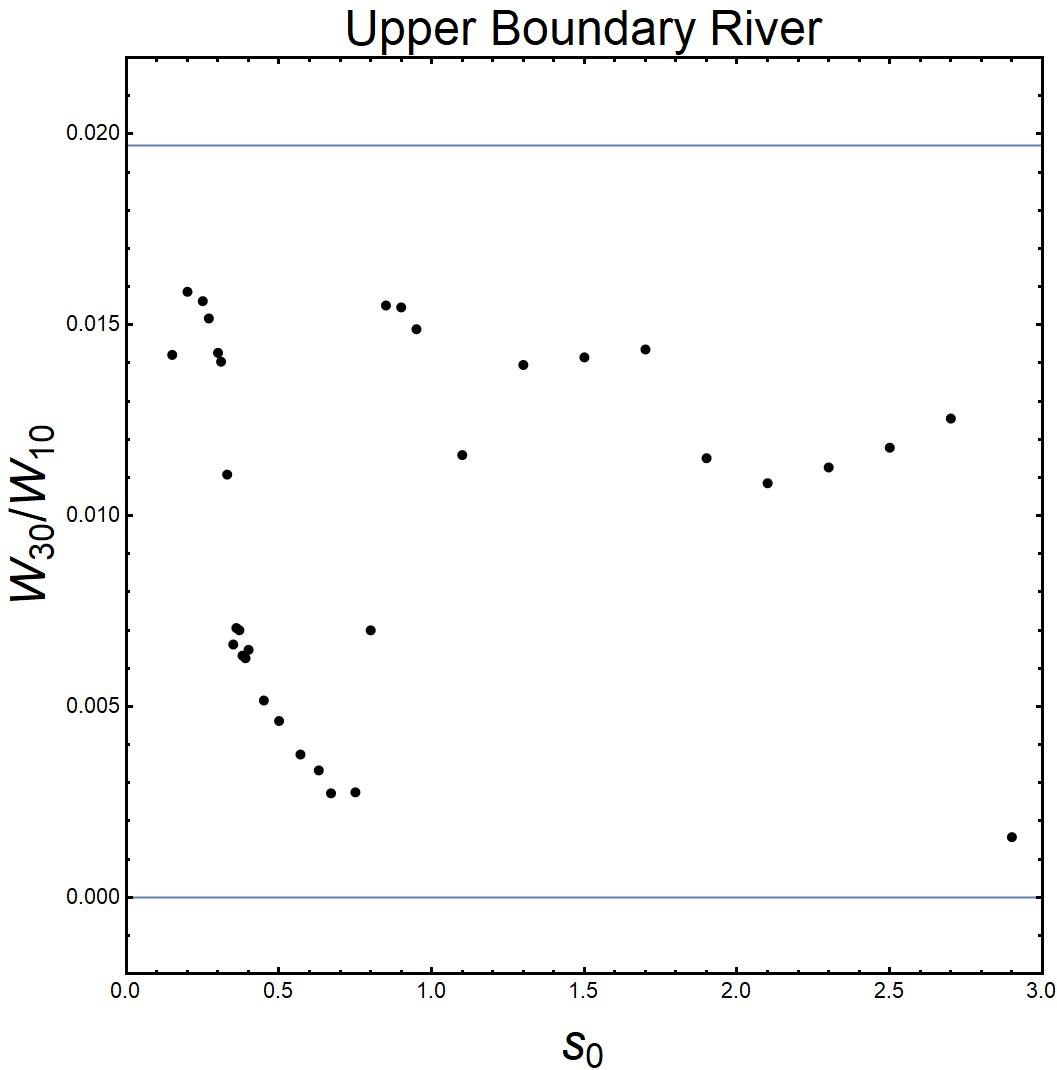
\includegraphics[width=6.7cm]{U30.jpg} }}
\end{figure}

\begin{figure}[H]
    \centering
   {{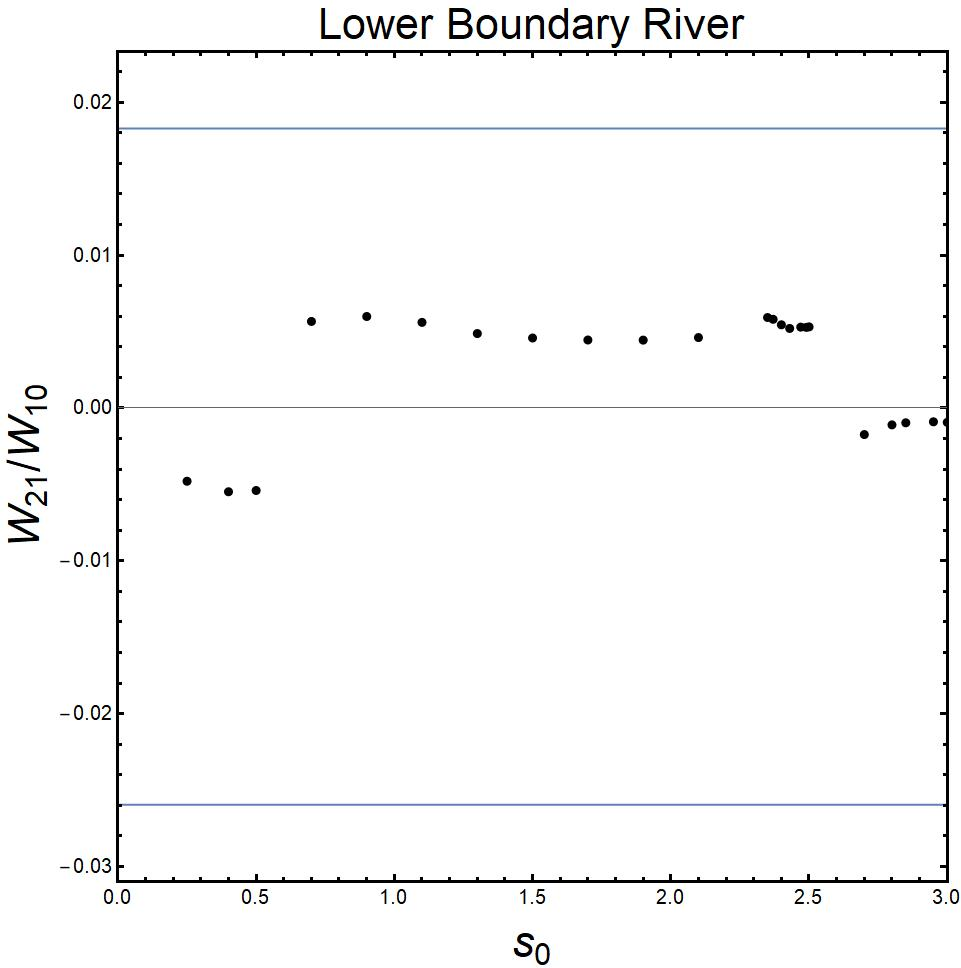
\includegraphics[width=6.7cm]{L21.jpg} }}
  {{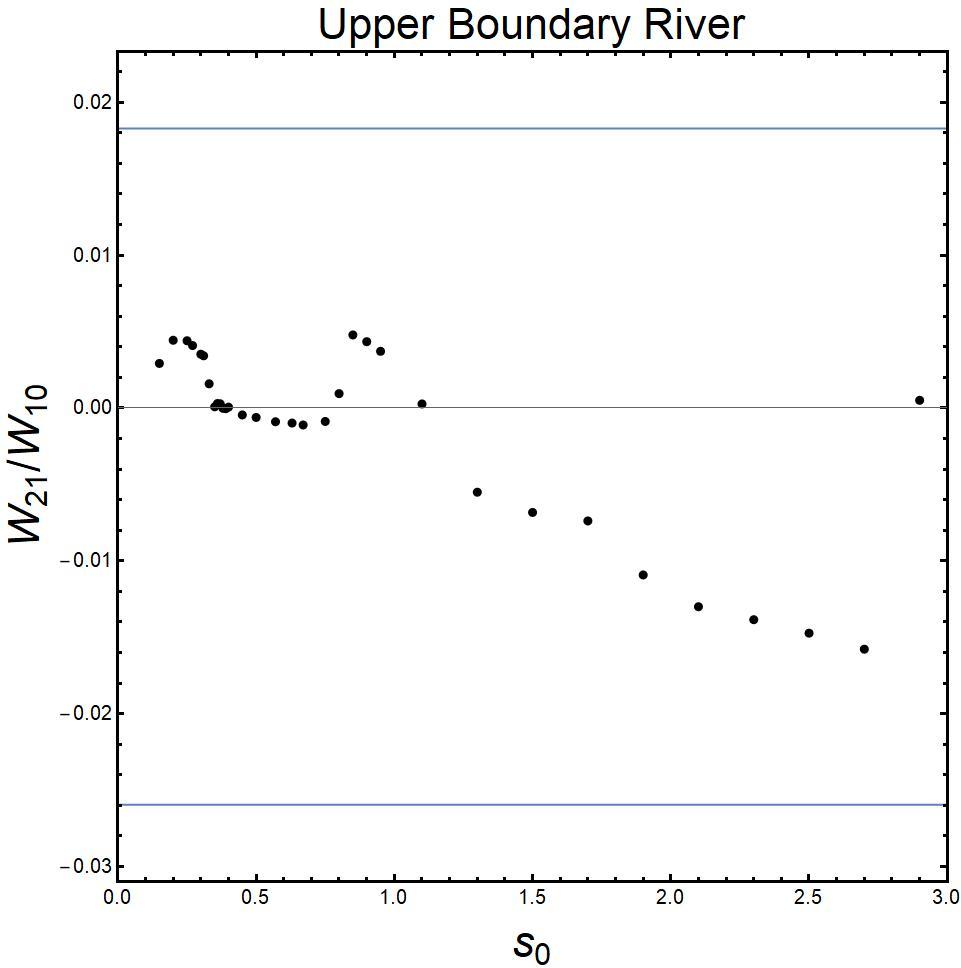
\includegraphics[width=6.7cm]{U21.jpg} }}
\end{figure}

\begin{figure}[H]
    \centering
   {{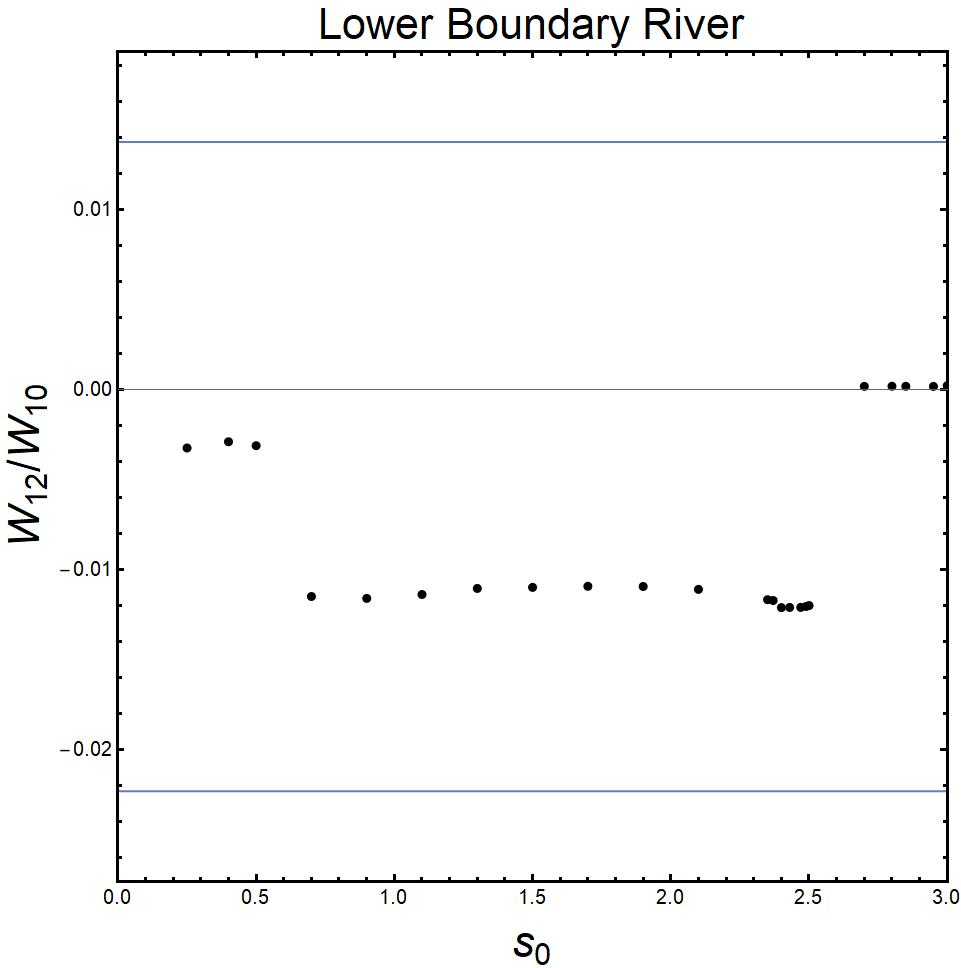
\includegraphics[width=6.7cm]{L12.jpg} }}
  {{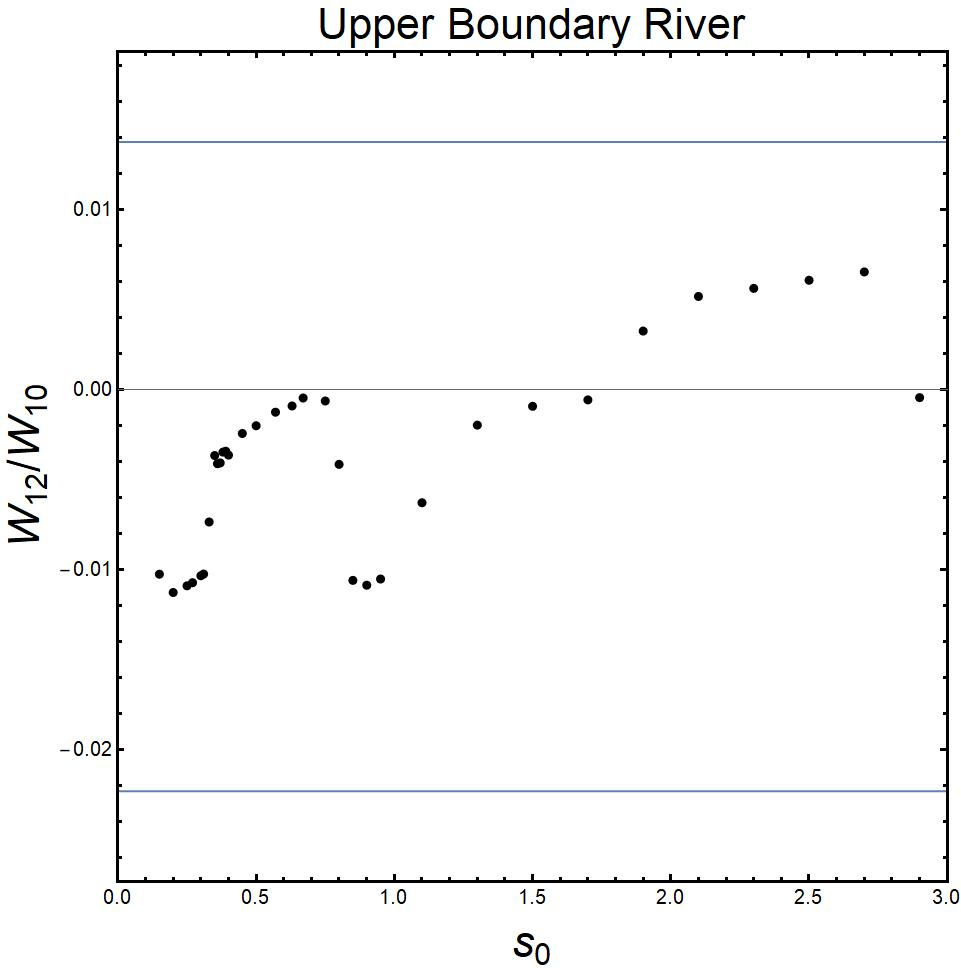
\includegraphics[width=6.7cm]{U12.jpg} }}
\end{figure}

\begin{figure}[H]
    \centering
   {{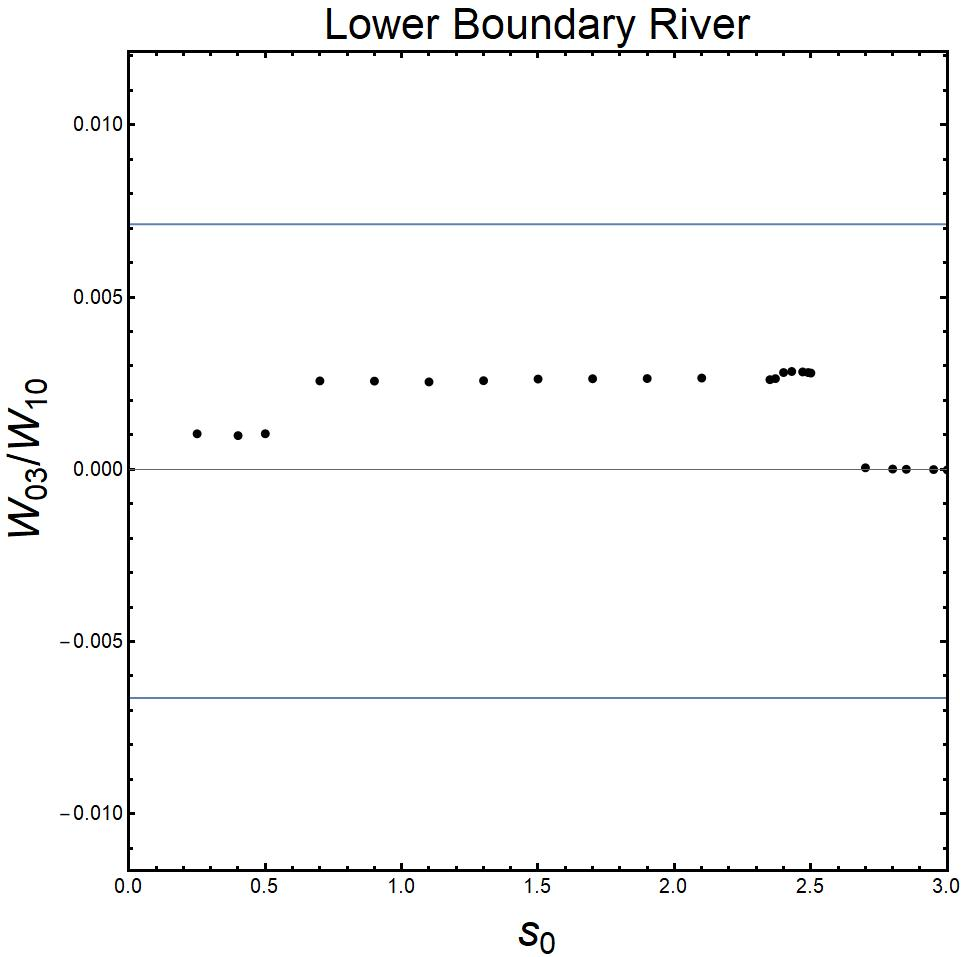
\includegraphics[width=6.7cm]{L03.jpg} }}
  {{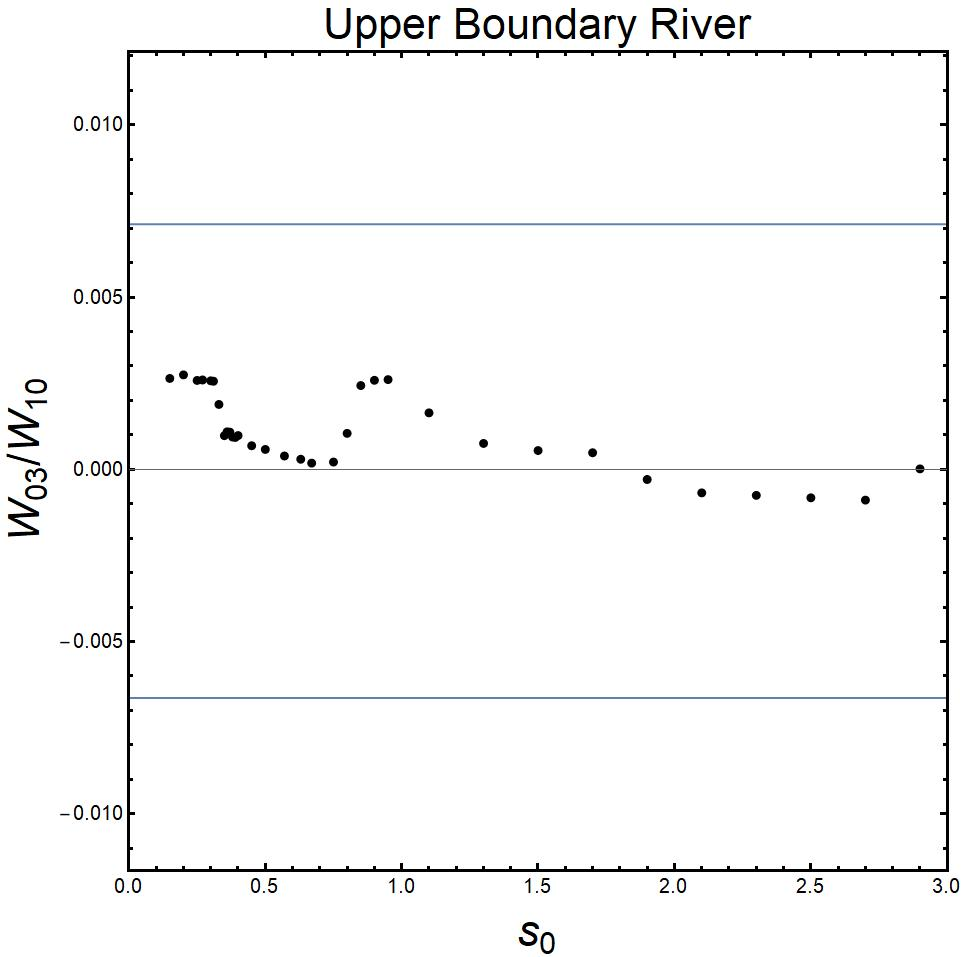
\includegraphics[width=6.7cm]{U03.jpg} }}
\end{figure}

\begin{figure}[H]
    \centering
   {{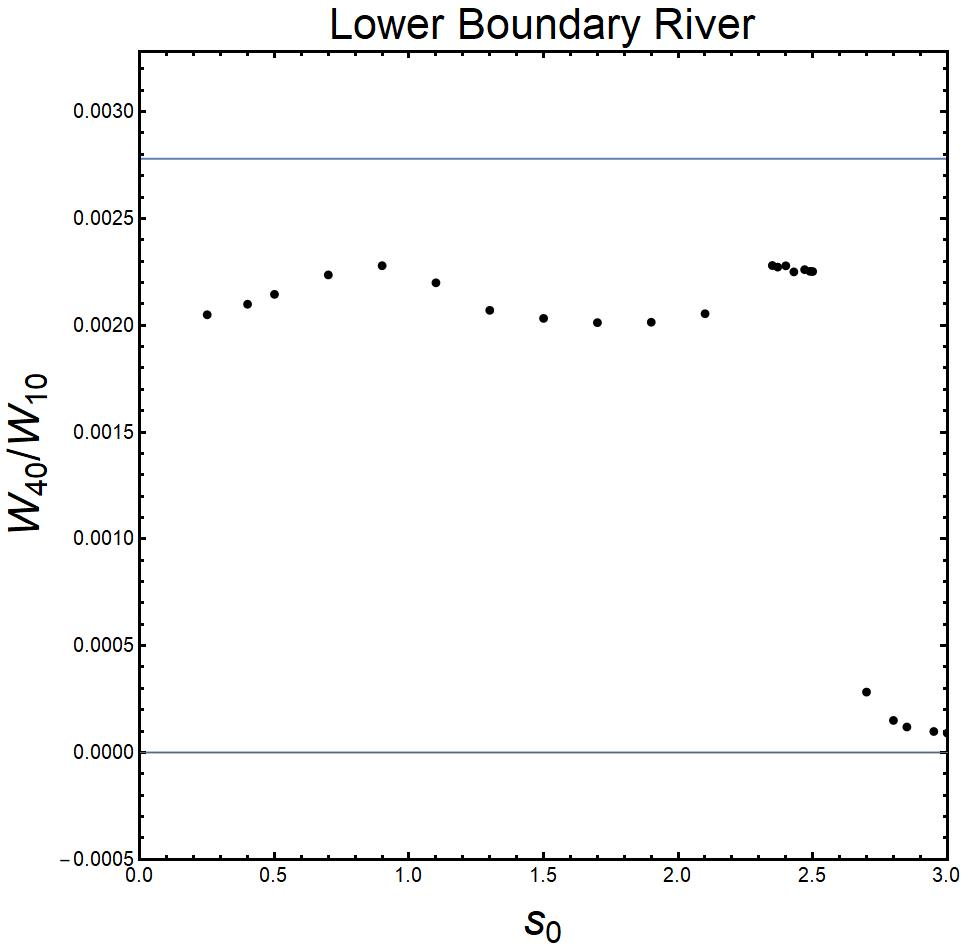
\includegraphics[width=6.7cm]{L40.jpg} }}
  {{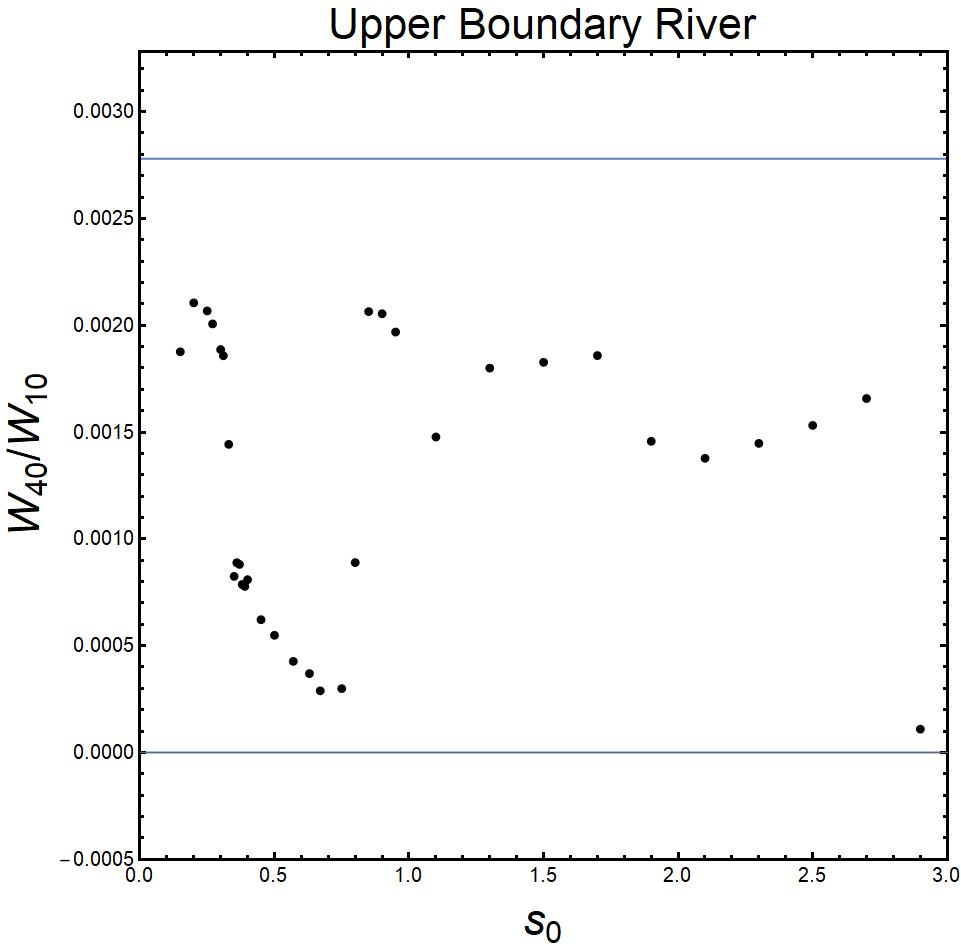
\includegraphics[width=6.7cm]{U40.jpg} }}
\end{figure}

\begin{figure}[H]
    \centering
   {{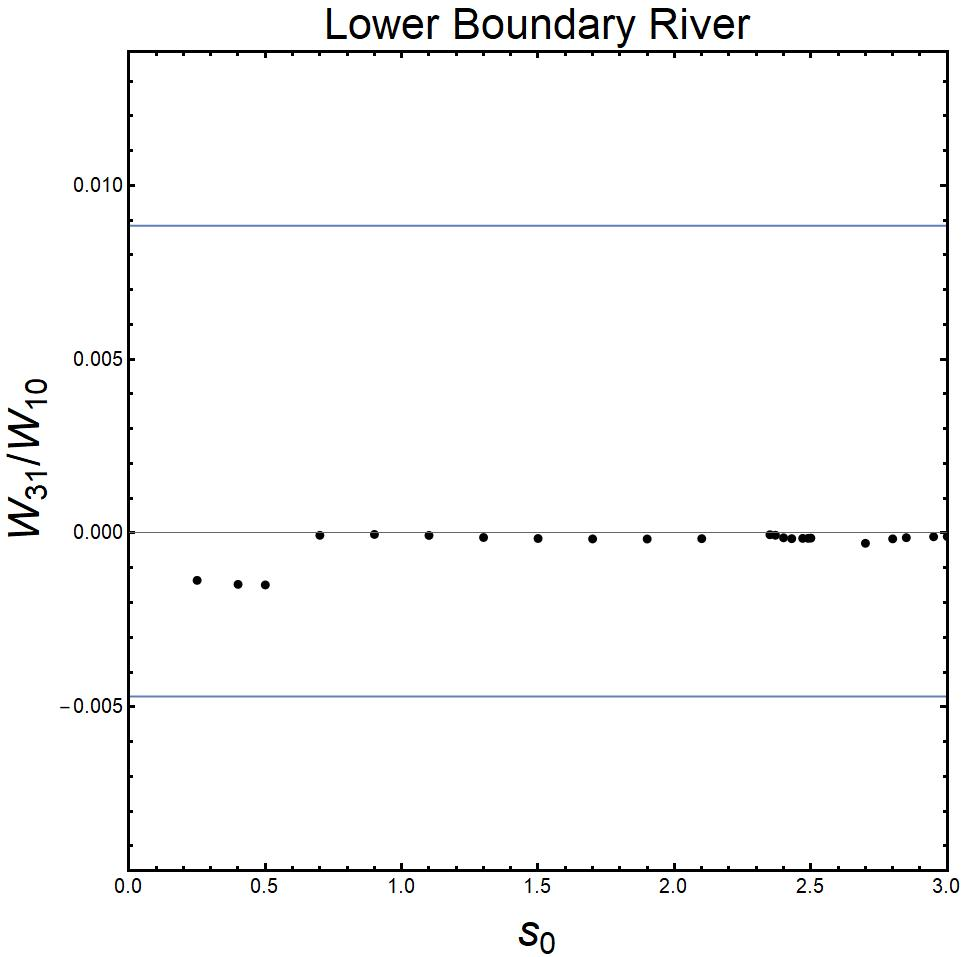
\includegraphics[width=6.7cm]{L31.jpg} }}
  {{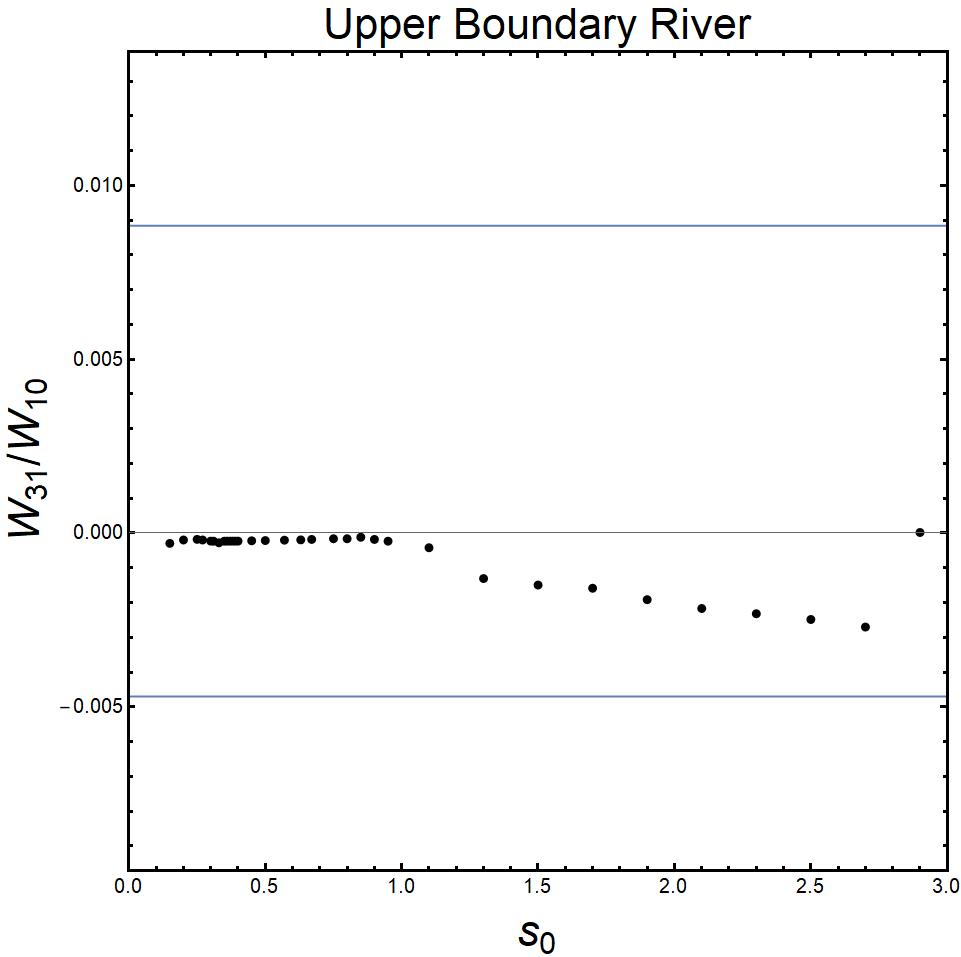
\includegraphics[width=6.7cm]{U31.jpg} }}
\end{figure}

\begin{figure}[H]
    \centering
   {{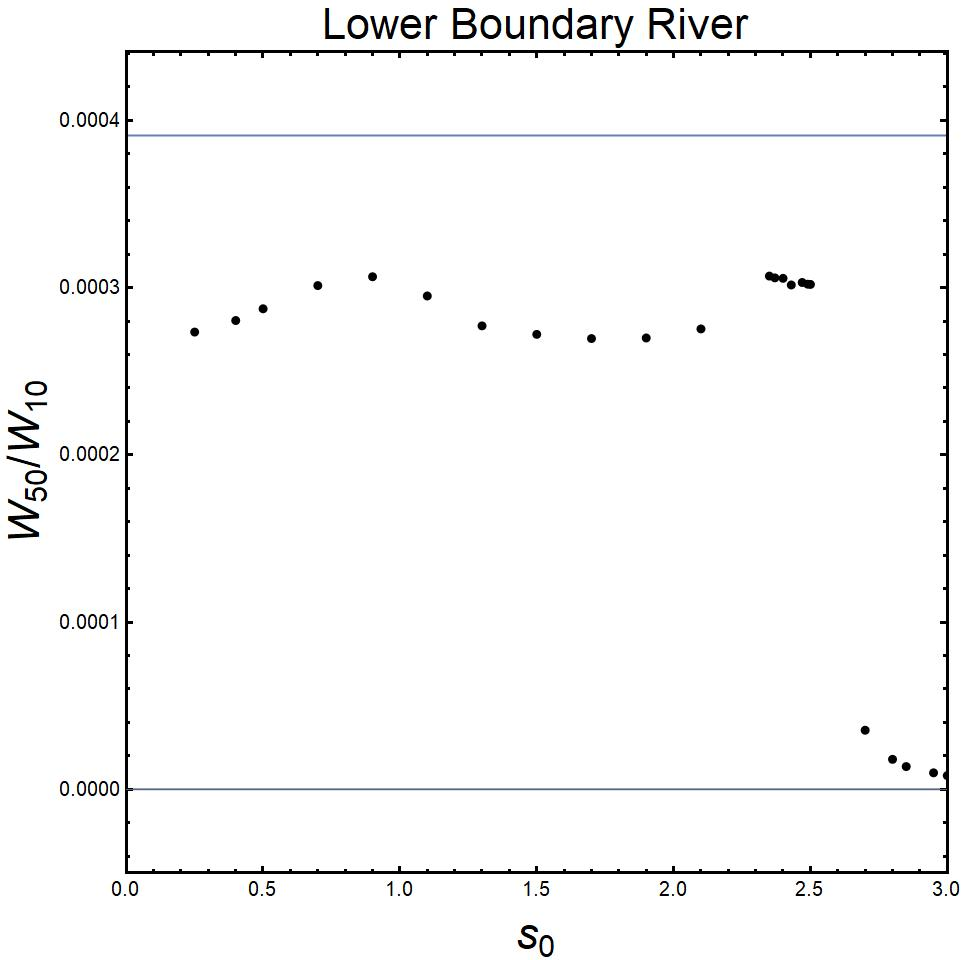
\includegraphics[width=6.7cm]{L50.jpg} }}
  {{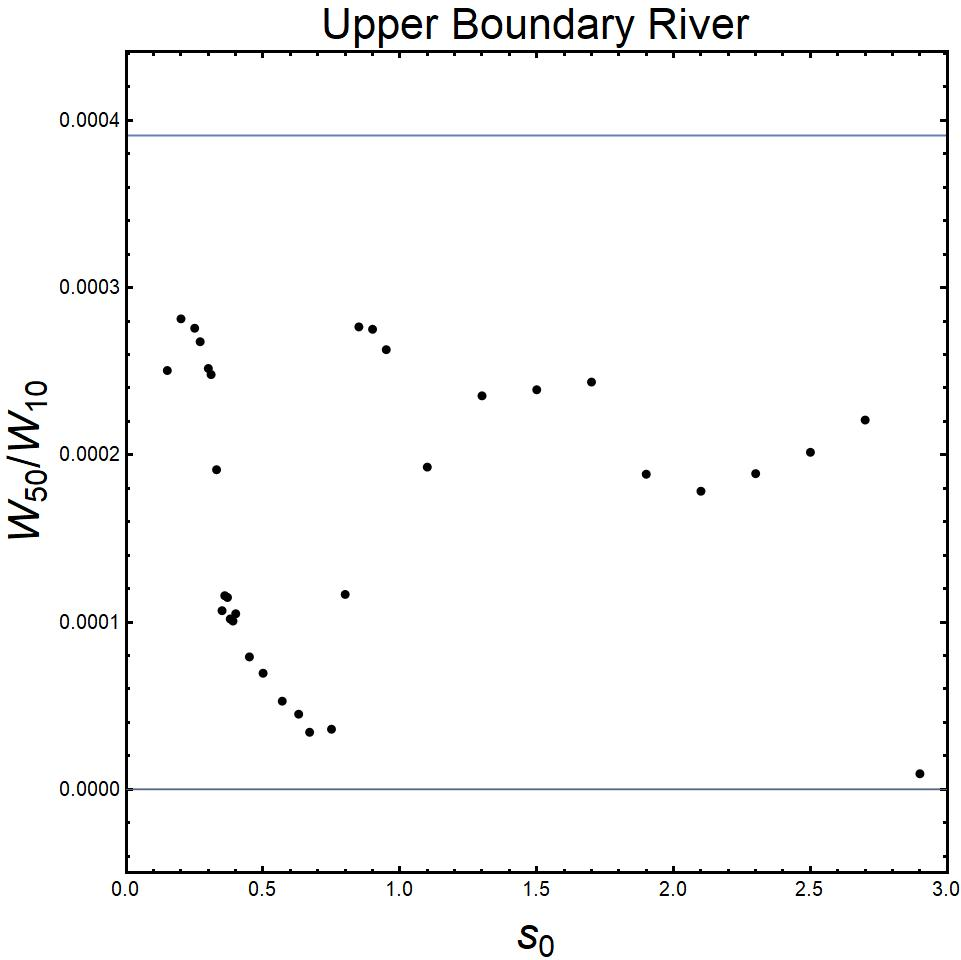
\includegraphics[width=6.7cm]{U50.jpg} }}
\end{figure}








\section{Conclusion}
In string bootstrap, only unitarity in different forms: 1. Partial wave unitarity, 2. Optical Theorem implying imaginary part of forward scattering amplitude is positive, 3. Unitarity at high energy, were used to contrain a Wilson coefficient $\alpha$ from below. Computation of higher $(N,L)$ needs to be done to get convergent values.\\\\
It will also be interesting to see how the values of Wilson coefficient ratios along various curves and boundaries depend on dimensions. For this, pion bootstrap will need to be implemented for higher dimensions. In the pion Lake we see that since resonance which is a strong coupling phenomenon is imposed, the tree level ChiPT Adler Zeroes are in the excluded pion Lake region which cannot accomodate resonances as a result of coupling not being strong enough. And since experimental value of $\rho$-resonance was used in 3+1D and this is uavailable for other dimensions, it will be interesting to see how different values of $m_{\rho}^{2}\in \mathbb{C}$ by varying both its real and imaginary parts will affect the lake boundary and other regions. Also higher dimensional pion bootstrap will require unitarity imposed at infinity separately as it will have factors of $s$ sitting in front of the $d(\cos\theta)$ integral which is divergent just like in string bootstrap case. The string bootstrap method for imposing this can be adapted to fit this purpose.\\\\
Moreover, other kinds of ratios like $\dfrac{\overline{W}_{p,q}}{\overline{W}_{1,0}}$ and $\dfrac{\widetilde W_{p,q}}{\widetilde W_{1,0}}$ can be studied with definitions
$$
A(s|t,u)=\sum_{p,q=0}^{\infty} \overline{W}_{p, q} (t+u)^{p} (tu)^{q} \qquad \qquad \text{(symmetric in $t$ and $u$)}
$$
$$
\mathcal{T}^{(2)}=A(t|s,u)+A(u|s,t)=\sum_{p,q=0}^{\infty} \widetilde W_{p, q} (t+u)^{p} (tu)^{q}
$$
which is again symmetric in $t$ and $u$ and since unlike $A(s|t,u)$, $\mathcal{T}^{(2)}$ is an isospin amplitude and also a physical scattering amplitude $\mathcal{M}(\pi^{+}\pi^{+}\rightarrow \pi^{+}\pi^{+})$ and hence its partial wave's imaginary part is expected to follow positivity ($a_{\ell}>0$) and hence is expected to follow bounds like the ratios discussed above. The relations between these new ratios and $W_{p,q}$'s can be found. 









\newpage
\appendix





\section{$s,t,u \mapsto \rho_{s},\rho_{t},\rho_{u}$}
We want to impose unitarity as $|S(s)|<1$. We do this using a technique given in \cite{5} . \\\\
We first consider $S$ as a function of $s,t$ ($u=0$ in 2D). We make the following transformation
$$
s \mapsto \rho_{s}=\frac{\sqrt{4 m^{2}-s_{0}}-\sqrt{4 m^{2}-s}}{\sqrt{4 m^{2}-s_{0}}+\sqrt{4 m^{2}-s}}, \quad s=\frac{s_{0}\left(1-\rho_{s}\right)^{2}+16 m^{2} \rho_{s}}{\left(1+\rho_{s}\right)^{2}}
$$
and similarily for $t$. And $s_{0}$ can be chosen to be $2m^{2}$, the symmetric point. The transformation maps the cut $s$-plane to a unit disk as shown in fig.  
\begin{figure}[H]
  \centering
  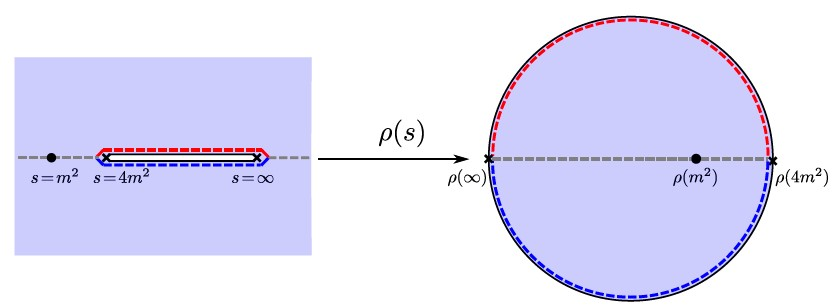
\includegraphics[width=\linewidth]{2.jpg}
  \caption{The mapping. From \cite{5}}
  \label{fig:1}
\end{figure}
The region $s \in\left[0,4 m^{2}\right]$ where all the poles reside are mapped to $\rho_{s} \in[2 \sqrt{2}-3,1]$. And apart from the poles, the S-matrix is analytic and hence can be written as 
$$
S(s, t)=\text{pole terms}+\sum_{a, b=0}^{\infty} c_{a b} \rho_{s}^{a} \rho_{t}^{b}
$$
Crossing symmetry $S(s,t)=S(t,s)$ needs $c_{a b}=c_{b a}$. Moreover we have the on-shell condition $s+t=4m^{2}$ which gives 
$$
\frac{s_{0}\left(1-\rho_{s}\right)^{2}+16 m^{2} \rho_{s}}{\left(1+\rho_{s}\right)^{2}}+\frac{s_{0}\left(1-\rho_{t}\right)^{2}+16 m^{2} \rho_{t}}{\left(1+\rho_{t}\right)^{2}}=4m^{2}
$$
$$
\Rightarrow \rho_{s}+\rho_{t}+4 \rho_{s} \rho_{t}+ \rho_{s}^{2} \rho_{t}+\rho_{s} \rho_{t}^{2}=0
$$
Defining $\rho^{(a, b)}=\rho_{s}^{a} \rho_{t}^{b}+$ permutations, we can rewrite this as
$$\rho^{(2,1)}+4 \rho^{(1,1)}+\rho^{(1,0)}=0$$
This can allow us to eliminate coefficients $c_{a b}$ by repeated redefinitions.\\\\
For $D=3$, $s_{0}=\frac{4}{3}$ ($m=1$) and $s,t,u$ are treated as independent to make the same transformation now for 3 variables and write 
$$
M(s, t, u)=\text{pole terms}+\sum_{a, b, c=0} \alpha_{a b c} \rho_{s}^{a} \rho_{t}^{b} \rho_{u}^{c}
$$
Crossing symmetry says $M$ is symmetric in all three indices and hence $\alpha$ is also symmetric in all 3 indices as a result. And on-shell condition here $s+t+u=4$, defining $\rho^{(a, b,c)}=\rho_{s}^{a} \rho_{t}^{b} \rho_{u}^{c}+$ permutations, boils down to 
$$\rho^{(2,2,1)}-4\rho^{(2,1,1)}+\rho^{(2,1,0)}+12\rho^{(1,1,1)}-4\rho^{(1,1,0)}-\rho^{(1,0,0)}=0$$




























\section{Integrating $P_{\ell}(x) \rho_{t}(s,x) \rho_{u}(s,x)$ w.r.t $x$ in 3+1D}
Following Appendix D.2 in \cite{5}, we wish to calculate the following integral which is needed to calculate the partial wave amplitudes to enter into SDPB.
$$
I_{b, c}^{\ell}=\int_{-1}^{1} \mathrm{~d} x P_{\ell}(x) \rho(t)^{b} \rho(u)^{c}
$$
Taking $s_{0}=\frac{4}{3}$,
$$
\rho_{s}=\frac{\sqrt{4-s_{0}}-\sqrt{4-s}}{\sqrt{4-s_{0}}+\sqrt{4-s}}=\frac{1-\sqrt{\frac{4-s}{4-s_{0}}}}{1+\sqrt{\frac{4-s}{4-s_{0}}}}
$$
and similarly for $\rho_{t}$ and $\rho_{u}$ with $t,u$ replacing $s$. Also $t=-\frac{1}{2}(s-4)(1-x)$ and $u=-\frac{1}{2}(s-4)(1+x)$, implies $4-t=4+\frac{1}{2}(s-4)(1-x)=\frac{s+4}{2}\left( 1-x\left(\frac{s-4}{s+4}\right) \right)$ and $4-u=4+\frac{1}{2}(s-4)(1+x)=\frac{s+4}{2}\left( 1+x\left(\frac{s-4}{s+4}\right) \right)$. This suggests defining 
$$
x=-\frac{s+4}{s-4} \cos (2 \phi)
$$
to get 
$$
\begin{aligned}
4-t&=\frac{s+4}{2}\left( 1+ \cos (2 \phi) \right)=(s+4) \cos^{2}\phi \\
4-u&=\frac{s+4}{2}\left( 1- \cos (2 \phi) \right)=(s+4) \sin^{2}\phi
\end{aligned}
$$
and further defining 
$$
r^{2} \equiv \frac{4+s}{4-s_{0}}
$$
$$
\sqrt{\frac{4-t}{4-s_{0}}}=r \cos \phi \qquad \sqrt{\frac{4-u}{4-s_{0}}}=r \sin \phi
$$
$$
\begin{aligned}
\rho_{t}&=\frac{1-\sqrt{\frac{4-t}{4-s_{0}}}}{1+\sqrt{\frac{4-t}{4-s_{0}}}}=\frac{1-r \cos \phi}{1+r \cos \phi}\\
\rho_{u}&=\frac{1-\sqrt{\frac{4-u}{4-s_{0}}}}{1+\sqrt{\frac{4-u}{4-s_{0}}}}=\frac{1-r \sin \phi}{1+r \sin \phi}
\end{aligned}
$$
$$
dx=4\left(\frac{s+4}{s-4}\right) \sin \phi \cos \phi d\phi=4\left(\frac{\frac{s+4}{4-s_{0}}}{\frac{s+4}{4-s_{0}}-\frac{8}{4-s_{0}}}\right) \sin \phi \cos \phi d\phi
$$
$$
dx=4\left(\frac{r^{2}}{r^{2}-\frac{8}{4-s_{0}}}\right) \sin \phi \cos \phi d\phi
$$
$$
\frac{s+4}{s-4}=\frac{r^{2}}{r^{2}-\frac{8}{4-s_{0}}}
$$
A new definition is made
$$
\phi=2 \arctan (y)
$$
$$
 \Rightarrow d \phi=2 \frac{1}{1+y^{2}} d y
$$
Since $y=\tan \left(\frac{\phi}{2} \right)$, \quad $\sin \phi=2 \left( \frac{y}{1+y^{2}}\right), \quad \cos \phi=\frac{1-y^{2}}{1+y^{2}} \quad \text{ and } \quad \cos(2\phi)=\frac{1-\left(\frac{2 y}{1-y^{2}}\right)^{2}}{1+\left(\frac{2 y}{1-y^{2}}\right)^{2}}=\frac{1-6 y^{2}+y^{4}}{\left(1+y^{2}\right)^{2}}$
$$
d x=16 \frac{r^{2}}{r^{2}-\frac{8}{4-s_{0}}} \frac{y\left(1-y^{2}\right)}{\left(1+y^{2}\right)^{3}} d y
$$
$$
x(y)=-\frac{r^{2}}{r^{2}-\frac{8}{4-s_{0}}} \frac{1-6 y^{2}+y^{4}}{\left(1+y^{2}\right)^{2}}
$$
$$
\begin{gathered}
\rho_{t}=\frac{1-r \cos \phi}{1+r \cos \phi}=\frac{1-r \frac{1-y^{2}}{1+y^{2}}}{1+r \frac{1-y^{2}}{1+y^{2}}}=\frac{(1-r)+y^{2}(1+r)}{(1+r)+y^{2}(1-r)} \\
\rho_{u}=\frac{1-r \sin \phi}{1+r \sin \phi}=\frac{1-r \frac{2 y}{1+y^{2}}}{1+r \frac{2 y}{1+y^{2}}}=\frac{1-2 r y+y^{2}}{1+2 r y+y^{2}}
\end{gathered}
$$
$$
I_{b, c}^{l}=16 \frac{r^{2}}{r^{2}-\frac{8}{4-s_{0}}} \int_{y_{i}}^{y_{f}} d y P_{l}(x(y)) \frac{y\left(1-y^{2}\right)}{\left(1+y^{2}\right)^{3}}\left(\frac{(1-r)+y^{2}(1+r)}{(1+r)+y^{2}(1-r)}\right)^{b}\left(\frac{1-2 r y+y^{2}}{1+2 r y+y^{2}}\right)^{c}
$$
As $x$ goes from -1 to 1, $y$ goes from 
$$
y_{i}=\frac{\sqrt{4-s_{0}}}{2}\left(r-\sqrt{r^{2}-\frac{4}{4-s_{0}}}\right)\quad \text{to} \quad y_{f}=\left(\frac{r-\frac{2}{4-s_{0}}}{r+\frac{2}{4-s_{0}}}\right)^{\frac{1}{2}}
$$
Using a trick involving discontinuity of logarithm, one can write
$$
\int_{y_{1}}^{y_{2}} \mathrm{~d} y f(y)=\frac{1}{2 \pi i} \int_{y_{1}}^{y_{2}} \mathrm{~d} y f(y) \operatorname{Disc} \log \left(\frac{y-y_{2}}{y-y_{1}}\right)=\frac{1}{2 \pi i} \int_{\left(y_{1}, y_{2}\right)} \mathrm{d} y f(y) \log \left(\frac{y-y_{2}}{y-y_{1}}\right)
$$
where the contour is a clockwise and wraps around the line segment from $y_{1}$ to $y_{2}$. Since $f(y)$ is a rational function, we know all its poles and this contour can else be bloated out to infinity and picks up the residues at these poles at $\pm i, \pm\left(\frac{r+1}{r-1}\right)^{\frac{1}{2}},-r \pm \sqrt{r^{2}-1}$ as contributions and this can be used to calculate the value of this integral.






















\section{Integrating $P^{(9)}_{\ell}(x) (1-x^{2})^{3}\rho_{t}(s,x) \rho_{u}(s,x)$ w.r.t $x$ in 9+1D}
It boils down to calculating
$$
I_{b, c}^{\ell}=\int_{-1}^{1} \mathrm{~d} x  (1-x^{2})^{3}\frac{C^{7/2}_{\ell}(x)}{C^{7/2}_{\ell}(1)} \rho(t)^{b} \rho(u)^{c}
$$
Taking $s_{0}=0.7$,
$$
\rho_{s}=\frac{\sqrt{s_{0}}-\sqrt{-s}}{\sqrt{s_{0}}+\sqrt{-s}}=\frac{1-\sqrt{\frac{-s}{s_{0}}}}{1+\sqrt{\frac{-s}{s_{0}}}}
$$
and similarly for $\rho_{t}$ and $\rho_{u}$ with $t,u$ replacing $s$. Also $t=-\frac{1}{2}s(1-x)$ and $u=-\frac{1}{2}s(1+x)$. This suggests defining
$$
x=- \cos (2 \phi)
$$
to get 
$$
\begin{aligned}
-t&=\frac{s}{2}\left( 1+ \cos (2 \phi) \right)=s \cos^{2}\phi \\
-u&=\frac{s}{2}\left( 1- \cos (2 \phi) \right)=s \sin^{2}\phi
\end{aligned}
$$
and further defining 
$$
r^{2} \equiv \frac{s}{s_{0}}
$$
$$
\sqrt{\frac{-t}{s_{0}}}=r \cos \phi \qquad \sqrt{\frac{-u}{s_{0}}}=r \sin \phi
$$
$$
\begin{aligned}
\rho_{t}&=\frac{1-\sqrt{\frac{-t}{s_{0}}}}{1+\sqrt{\frac{-t}{s_{0}}}}=\frac{1-r \cos \phi}{1+r \cos \phi}\\
\rho_{u}&=\frac{1-\sqrt{\frac{-u}{s_{0}}}}{1+\sqrt{\frac{-u}{s_{0}}}}=\frac{1-r \sin \phi}{1+r \sin \phi}
\end{aligned}
$$
$$
dx=4 \sin \phi \cos \phi d\phi
$$
A new definition is made
$$
\phi=2 \arctan (y)
$$
$$
 \Rightarrow d \phi=2 \frac{1}{1+y^{2}} d y
$$
Since $y=\tan \left(\frac{\phi}{2} \right)$, \quad $\sin \phi=2 \left( \frac{y}{1+y^{2}}\right), \quad \cos \phi=\frac{1-y^{2}}{1+y^{2}} \quad \text{ and } \quad \cos(2\phi)=\frac{1-\left(\frac{2 y}{1-y^{2}}\right)^{2}}{1+\left(\frac{2 y}{1-y^{2}}\right)^{2}}=\frac{1-6 y^{2}+y^{4}}{\left(1+y^{2}\right)^{2}}$
$$
d x=16 \frac{y\left(1-y^{2}\right)}{\left(1+y^{2}\right)^{3}} d y
$$
$$
x(y)=- \frac{1-6 y^{2}+y^{4}}{\left(1+y^{2}\right)^{2}}
$$
$$
(1-x^{2})^{3}=(1-\cos(2\phi))^{3}=\sin^{6}(2\phi)=2^{6}\left( \frac{2y}{1+y^{2}} \right)^{6} \left(\frac{1-y^{2}}{1+y^{2}} \right)^{6}=2^{12} \left(\frac{y(1-y^{2})}{(1+y^{2})^{2}} \right)^{6}
$$
$$
\begin{gathered}
\rho_{t}=\frac{1-r \cos \phi}{1+r \cos \phi}=\frac{1-r \frac{1-y^{2}}{1+y^{2}}}{1+r \frac{1-y^{2}}{1+y^{2}}}=\frac{(1-r)+y^{2}(1+r)}{(1+r)+y^{2}(1-r)} \\
\rho_{u}=\frac{1-r \sin \phi}{1+r \sin \phi}=\frac{1-r \frac{2 y}{1+y^{2}}}{1+r \frac{2 y}{1+y^{2}}}=\frac{1-2 r y+y^{2}}{1+2 r y+y^{2}}
\end{gathered}
$$
$$
I_{b, c}^{l}=2^{16} \int_{y_{i}}^{y_{f}} d y \frac{C^{7/2}_{\ell}(x(y))}{C^{7/2}_{\ell}(1)}\left(\frac{y(1-y^{2})}{(1+y^{2})^{2}} \right)^{6} \frac{y\left(1-y^{2}\right)}{\left(1+y^{2}\right)^{3}}\left(\frac{(1-r)+y^{2}(1+r)}{(1+r)+y^{2}(1-r)}\right)^{b}\left(\frac{1-2 r y+y^{2}}{1+2 r y+y^{2}}\right)^{c}
$$
As $x$ goes from -1 to 1, $\phi$ goes from $\pi/2$ to $0$ and $y$ goes from $y_{i}=0$ to $y_{f}=1$
Using a trick involving discontinuity of logarithm, one can write
$$
\int_{y_{1}}^{y_{2}} \mathrm{~d} y f(y)=\frac{1}{2 \pi i} \int_{y_{1}}^{y_{2}} \mathrm{~d} y f(y) \operatorname{Disc} \log \left(\frac{y-y_{2}}{y-y_{1}}\right)=\frac{1}{2 \pi i} \int_{\left(y_{1}, y_{2}\right)} \mathrm{d} y f(y) \log \left(\frac{y-y_{2}}{y-y_{1}}\right)
$$
where the contour is a clockwise and wraps around the line segment from $y_{1}$ to $y_{2}$. Since $f(y)$ is a rational function, we know all its poles and this contour can else be bloated out to infinity and picks up the residues at these poles (at $\pm i, \pm\left(\frac{r+1}{r-1}\right)^{\frac{1}{2}},-r \pm \sqrt{r^{2}-1}$ if $s>s_{0}$ and $\pm i, \pm i\left(\frac{1+r}{1-r}\right)^{\frac{1}{2}},-r \pm i\sqrt{1-r^{2}}$ if $s<s_{0}$) as contributions and this can be used to calculate the value of this integral.\\\\
It turns out that for roughly $l>25$ onwards, brute force NIntegrate is faster than calculating residues but for lower $l$, residue calculation is faster. So a cutoff of $l \approx 25$ can be used since for string bootstrap, even for something like $N_{max}=13$, one needs to go upto $L_{max}=70$ for convergence.\\\\
Also residue at $\pm i$ takes most of the time and time can be halved by using $2\operatorname{Re}$[Residue at $i$].

















\bibliographystyle{plain}
\bibliography{references}






\end{document}

